\documentclass{article}

\usepackage{arxiv}

\usepackage[utf8]{inputenc} % allow utf-8 input
\usepackage[T1]{fontenc}    % use 8-bit T1 fonts
\usepackage{lmodern}        % https://github.com/rstudio/rticles/issues/343
\usepackage{hyperref}       % hyperlinks
\usepackage{url}            % simple URL typesetting
\usepackage{booktabs}       % professional-quality tables
\usepackage{amsfonts}       % blackboard math symbols
\usepackage{nicefrac}       % compact symbols for 1/2, etc.
\usepackage{microtype}      % microtypography
\usepackage{graphicx}

\title{Introducing ICBe: An Event Extraction Dataset from Narratives
about International Crises}

\author{
    Rex W. Douglass
    \thanks{Correspondence should be addressed to Rex W. Douglass at
\href{mailto:rexdouglass@gmail.com}{\nolinkurl{rexdouglass@gmail.com}}.}
   \\
    University of California, San Diego \\
   \\
  \texttt{} \\
   \And
    Thomas Leo Scherer
   \\
    University of California, San Diego \\
   \\
  \texttt{} \\
   \And
    J Andrés Gannon
   \\
    Vanderbilt University \\
   \\
  \texttt{} \\
   \And
    Erik Gartzke
   \\
    University of California, San Diego \\
   \\
  \texttt{} \\
   \And
    Jon Lindsay
   \\
    Georgia Institute of Technology \\
   \\
  \texttt{} \\
   \And
    Shannon Carcelli
   \\
    University of Maryland \\
   \\
  \texttt{} \\
   \And
    Jonathan Wilkenfeld
   \\
    University of Maryland \\
   \\
  \texttt{} \\
   \And
    David M. Quinn
   \\
    University of Maryland \\
   \\
  \texttt{} \\
   \And
    Catherine Aiken
   \\
    Georgetown University \\
   \\
  \texttt{} \\
   \And
    Jose Miguel Cabezas Navarro
   \\
    Universidad Mayor \\
   \\
  \texttt{} \\
   \And
    Neil Lund
   \\
    University of Maryland \\
   \\
  \texttt{} \\
   \And
    Egle Murauskaite
   \\
    University of Maryland \\
   \\
  \texttt{} \\
   \And
    Diana Partridge
   \\
    University of Maryland \\
   \\
  \texttt{} \\
  }


% tightlist command for lists without linebreak
\providecommand{\tightlist}{%
  \setlength{\itemsep}{0pt}\setlength{\parskip}{0pt}}


% Pandoc citation processing
\newlength{\cslhangindent}
\setlength{\cslhangindent}{1.5em}
\newlength{\csllabelwidth}
\setlength{\csllabelwidth}{3em}
\newlength{\cslentryspacingunit} % times entry-spacing
\setlength{\cslentryspacingunit}{\parskip}
% for Pandoc 2.8 to 2.10.1
\newenvironment{cslreferences}%
  {}%
  {\par}
% For Pandoc 2.11+
\newenvironment{CSLReferences}[2] % #1 hanging-ident, #2 entry spacing
 {% don't indent paragraphs
  \setlength{\parindent}{0pt}
  % turn on hanging indent if param 1 is 1
  \ifodd #1
  \let\oldpar\par
  \def\par{\hangindent=\cslhangindent\oldpar}
  \fi
  % set entry spacing
  \setlength{\parskip}{#2\cslentryspacingunit}
 }%
 {}
\usepackage{calc}
\newcommand{\CSLBlock}[1]{#1\hfill\break}
\newcommand{\CSLLeftMargin}[1]{\parbox[t]{\csllabelwidth}{#1}}
\newcommand{\CSLRightInline}[1]{\parbox[t]{\linewidth - \csllabelwidth}{#1}\break}
\newcommand{\CSLIndent}[1]{\hspace{\cslhangindent}#1}

\usepackage[utf8]{inputenc}
\usepackage{pifont}
\usepackage{newunicodechar}
\newunicodechar{✓}{\ding{51}}
\newunicodechar{✗}{\ding{55}}
\usepackage{array}
\usepackage{ctable}
\usepackage{booktabs}
\usepackage{longtable}
\usepackage{array}
\usepackage{multirow}
\usepackage{wrapfig}
\usepackage{colortbl}
\usepackage{pdflscape}
\usepackage{tabu}
\usepackage{threeparttable}
\usepackage{threeparttablex}
\usepackage[normalem]{ulem}
\usepackage{makecell}
\usepackage{titlesec}
\usepackage[parfill]{parskip}
\usepackage{makecell}
\usepackage{graphicx}
\usepackage{setspace}
\usepackage{cellspace}
\setlength\cellspacetoplimit{0.8ex}
\renewcommand{\arraystretch}{0.8}
\AtBeginEnvironment{lltable}{\singlespacing}
\usepackage{subcaption}
\usepackage{atbegshi}% http://ctan.org/pkg/atbegshi
\usepackage{float}
\usepackage[algo2e]{algorithm2e}
\usepackage{changepage}
\renewcommand{\bibliography}[1]{}
\usepackage{multirow}
\usepackage{multicol}
\usepackage{colortbl}
\usepackage{hhline}
\newlength\Oldarrayrulewidth
\newlength\Oldtabcolsep
\usepackage{longtable}
\usepackage{array}
\usepackage{hyperref}
\begin{document}
\maketitle


\begin{abstract}
How do international crises unfold? We conceptualize international
relations as a strategic chess game between adversaries and develop a
systematic way to measure pieces, moves, and gambits accurately and
consistently over a hundred years of history. We introduce a new
ontology and dataset of international events called ICBe based on a very
high-quality corpus of narratives from the International Crisis Behavior
(ICB) Project. We demonstrate that ICBe has higher coverage, recall, and
precision than existing state of the art datasets and conduct two
detailed case studies of the Cuban Missile Crisis (1962) and the
Crimea-Donbas Crisis (2014). We further introduce two new event
visualizations (event iconography and crisis maps), an automated
benchmark for measuring event recall using natural language processing
(synthetic narratives), and an ontology reconstruction task for
objectively measuring event precision. We make the data, supplementary
appendix, replication material, and visualizations of every historical
episode available at a companion website crisisevents.org.
\end{abstract}


\doublespacing
\newpage

If we could record every international interaction in the realms of
diplomacy, conflict, economics, and beyond, how much unique information
would this chronicle amount to, and how surprised would we be to see
something new? In other words, what is the entropy of international
relations? While this record could in principle be unbounded, the
central conceit of social science is that there are structural
regularities that limit what actors can do, their best options, and even
which actors are likely to survive (Brecher 1999; Reiter 2015). If so,
then these events can be recorded and systematically measured by social
scientists interested in these regularities.\footnote{See work on crises
  (Brecher and Wilkenfeld 1982; Beardsley et al. 2020), militarized
  disputes (Palmer et al. 2021; Gibler 2018), wars (Sarkees and Wayman
  2010; Reiter, Stam, and Horowitz 2016), organized violence (Ralph
  Sundberg and Mihai Croicu 2016; Davies, Pettersson, and Öberg 2022),
  political violence (Raleigh et al. 2010), sanctions (Felbermayr et al.
  2020), and international agreements (Kinne 2020; Owsiak, Cuttner, and
  Buck 2018), dispute resolution (Frederick, Hensel, and Macaulay 2017),
  and diplomacy (Moyer, Turner, and Meisel 2020; Sechser 2011).} Thanks
to improvements in natural language processing, more open-ended efforts
have begun to capture entire unstructured streams of events from
international news reports.\footnote{See Beieler et al. (2016); Boschee
  et al. (2015); Brandt et al. (2018); Grant et al. (2017); Li et al.
  (2021). On event extraction from images and social media see Zhang and
  Pan (2019) and Steinert-Threlkeld (2019).} This has invited fruitful
efforts to evaluate the coverage, quality, and accuracy of attempts to
measure international affairs.

We advance existing efforts to identify and structure regularized events
and actor in international politics by combining human coding with
natural language processing to develop (1) a large, flexible ontology of
international affairs and (2) a fine-grained and structured event
dataset of international crises from 1918-2017 developed by applying our
ontology to an unusually high-quality corpus of historical narratives of
international crises (Brecher 1999; Wilkenfeld and Brecher 2000; Brecher
et al. 2021). We then develop several methods for objectively gauging
how well these event codings reconstruct the information contained in
the original crisis narrative. We conclude by benchmarking our event
codings against several current state of the art event data collection
efforts. The underlying fine-grained variation in international affairs
is unrecognizable through the lens of current quantification efforts. We
find that existing models produce data on historical episodes that do
not contain enough information to reconstruct the underlying event. In
focusing this initial effort on international crises as a proof of
concept sample, we demonstrate our ontology and method's potential to
improve upon existing empirical identifications of patterns of
international interactions.

In the proceeding four sections, this measurement paper makes the
following arguments. First, there is a real-world unobserved latent
concept known as international relations that can and should be
systematically measured. Second, we propose a method for systematic
large-scale measurement of the actors and behaviors in international
affairs and as a proof of concept apply that method to a well-regarded
and salient sample of events known as international crises. Third, in
doing so we confirm that those measurements exhibit several desirable
kinds of internal and external validity and out-perform existing
approaches. Fourth, this validation can be evaluated in detail via new
event visualizations, with examples provided for case studies of the
1962 Cuban Missile Crisis and 2014 Crimea-Donbas crisis. A final section
concludes.

\hypertarget{identifying-and-measuring-international-relations}{%
\section{Identifying and measuring international
relations}\label{identifying-and-measuring-international-relations}}

\hypertarget{motivation}{%
\subsection{Motivation}\label{motivation}}

How can scholars abstract and measure discrete events about a historical
episode in international relations? We employ a metaphor of chess, a
game that despite its complexity can nonetheless be recorded in a
standardized and structured manner. Like chess, international
interactions involve a finite set of players (e.g.~polities, rebel
groups, IGOs) expressing their behaviors (e.g.~thinking, saying, and
doing) by moving pieces (e.g.~military platforms, civilian personnel,
diplomats) from and onto identifiable locations (geo-coded coordinates).
These moves occur over a marked time period (start and end of a
historical episode) and gambits occur in recordable sequences (actions
and reactions) to produce observable, if still disputable, outcomes
(e.g.~victory, defeat, stalemate, peace). Our knowledge of this
historical episode, including the actors involved as well as their
preferences, behaviors, and beliefs are only indirectly observed from
historical records that most often take the form of unstructured natural
language text.

Much like the recording of chess evolved from natural language
descriptive text notation to the modern figurine algebra notion,
international relations scholars have recently sought to produce a
structured account of historical events by combining the unstructured
corpus of historical records with informative priors about international
relations. The resulting structured account of information about a
historical episode can be combined with that of other events to produce
a systematic account of political events from which we can garner novel
insight, assuming the underlying data have high coverage, precision, and
recall. The easiest way to convey the desired produced of this task is
with an example. Figure 1 shows a narrative account of the Cuban Missile
Crisis (1962) in natural language sentences alongside a mapping to
discrete machine-readable abstractive events. From the structured data,
scholars can identify similarities and differences across events
concerning important concepts like when particular foreign policy
actions deter versus inflame (Jervis 1978; Glaser 2000), when third
parties mediate in interstate disputes (Haffar 2002; Quinn et al. 2006),
and how actors try to communicate resolve (Trager 2016; Lupton 2018).
Identifying patterns of international interactions is not just an
inherently interesting enterprise; it is a necessary precondition to
important efforts to predict where policymakers should turn their
attention to improve global welfare (Ward et al. 2013; Beger, Morgan,
and Ward 2021).

\begin{figure}
\hypertarget{fig-cubanarrative}{%
\centering
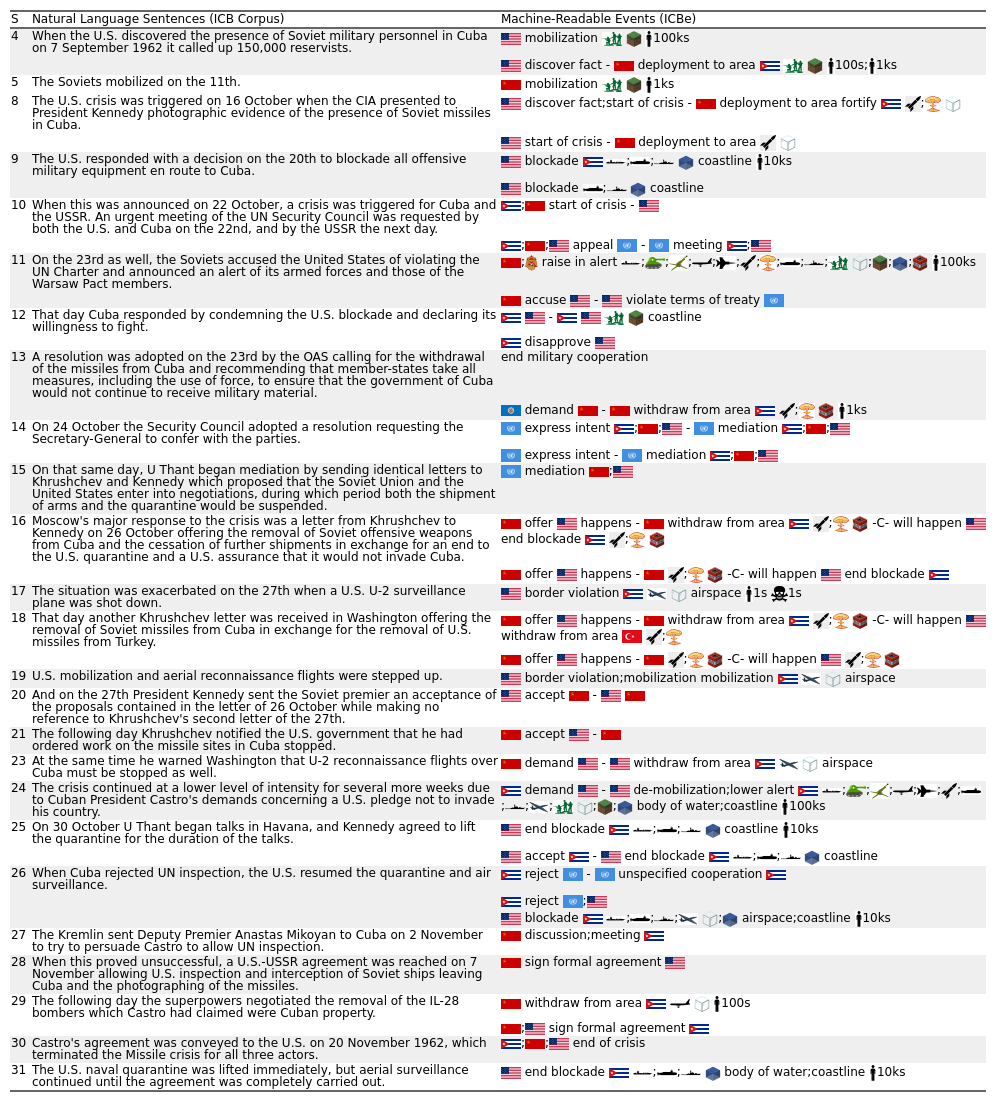
\includegraphics[width=7in,height=8in]{case_study_cuban_precision.png}
\caption{Cuban Missile Crisis (1962) - ICB Narrative vs.~ICBe
Events}\label{fig-cubanarrative}
}
\end{figure}

\hypertarget{existing-state-of-the-art-measurements}{%
\subsection{Existing state of the art
measurements}\label{existing-state-of-the-art-measurements}}

We draw informative prior beliefs about the underlying process of
international relations that we expect to govern behavior during
historical episodes and their conversion to the historical record. We
organize our prior beliefs along two overarching axes: existing efforts
to identify the actors/actions of international relations and
identifying a corpus that can be used to produce an ontology of the
information we hope to recover. Table 1 describes these two axes as
columns and rows, respectively.

The rows in Table 1 represent the types of information we expect to find
in international relations and forms the basis for our proposed
ontology. We created this ontology by performing of the corpus and
identifying named entities and verbs mentioned in the text. To identify
possible behaviors, we matched verbs to the most likely definition found
in Wordnet (Miller 1995), tallied (SI Appendix 1.2), and then aggregated
them into a smaller number of behaviors balancing conceptual detail with
manageable sparsity for human coding, informed by existing conceptual
(``Literature'' column) and measurement research (discussed below). We
used the ICB project actor level data to identify likely actors for each
crisis and location options relative to each actor. For behavior, actor,
and location, coders could write-in a value if the given options were
insufficient. The codebook lists 11 behaviors added post-coding as
coders flagged events that were not captured by the initial ontology
(e.g.~propaganda).

As we are not the first to attempt to measure international relations in
a structured manner, the columns of Table 1 compare the ontological
coverage of ICBe to existing state of the art systems in production and
with global coverage. We choose these datasets and models as they
represent frequently used and reputable efforts to structure and
describe historical events of interest to scholars of international
politics. The first column starts with our contribution, ICBe, alongside
other event-level datasets including CAMEO dictionary lookup-based
systems (Historical Phoenix (Althaus et al. 2019); ICEWS (Boschee et al.
2015); Terrier (Grant et al. 2017)), the Militarized Interstate Disputes
Incidents dataset, the UCDP-GED dataset (Davies, Pettersson, and Öberg
2022; Sundberg and Melander 2013), and ACLED (Raleigh et al.
2010).\footnote{Other related datasets that insufficiently overlap
  ICBe's domain for comparison include BCOW (Leng and Singer 1988), WEIS
  (McClelland 1978), CREON (Hermann 1984), CASCON (Bloomfield and
  Moulton 1989), SHERFACS (Sherman 2000), Real-Time Phoenix (Brandt et
  al. 2018), and COfEE (Balali, Asadpour, and Jafari 2021) (see
  histories in Merritt (1994) and Schrodt and Hall (2006)).} The final
set of columns compares episode-level datasets beginning with the
original ICB project (Brecher et al. 2021; Brecher and Wilkenfeld 1982;
Beardsley et al. 2020); the Militarized Interstate Disputes dataset
(Palmer et al. 2021; Gibler 2018), and the Correlates of War (Sarkees
and Wayman 2010). We include episode-level datasets as they remain and
common and trusted tool for analyzing international relations, and
because ICBe is unique among event-level datasets as events are matched
to crises and so can be aggregated to the episode level. There is
imperfect overlap concerning their intended depth and scope of coverage;
`international crises' are similar, but not identical to, `interstate
wars' and `militarized interstate disputes' which differ yet again from
`individual events of organized violence' and `non-violent action'. Even
like-concepts require care in comparison, as an `aim' in ICBe is the
same as in MIPS, but an `alert' in ICBe is not the same as an `alert' in
MID.

This comparison is not intended to fault existing data and models for
not including every variable in ICBe's ontology, as some of these
variables fall outside the scope of a particular dataset's intended
purpose. Rather, it serves as an initial basis for identifying the
heterogeneity in existing efforts to abstract and measure discrete
historical events of interest and to provide theoretical justifications
from existing research about what is included in our dataset's ontology
and where ICBe's detail about historical events can be compared to the
current state of the art.

\clearpage
\singlespacing

\global\setlength{\Oldarrayrulewidth}{\arrayrulewidth}

\global\setlength{\Oldtabcolsep}{\tabcolsep}

\setlength{\tabcolsep}{0pt}

\renewcommand*{\arraystretch}{1}



\providecommand{\ascline}[3]{\noalign{\global\arrayrulewidth #1}\arrayrulecolor[HTML]{#2}\cline{#3}}

\begin{longtable}[c]{|p{0.10in}|p{1.80in}|p{1.50in}|p{0.25in}|p{0.25in}|p{0.25in}|p{0.25in}|p{0.25in}|p{0.25in}|p{0.25in}|p{0.25in}|p{0.25in}|p{0.25in}}

\caption{Ontological\ coverage\ of\ ICBe\ versus\ existing\ State\ of\ the\ Art}\\

\hhline{>{\arrayrulecolor[HTML]{000000}\global\arrayrulewidth=2pt}->{\arrayrulecolor[HTML]{000000}\global\arrayrulewidth=2pt}->{\arrayrulecolor[HTML]{000000}\global\arrayrulewidth=2pt}->{\arrayrulecolor[HTML]{000000}\global\arrayrulewidth=2pt}->{\arrayrulecolor[HTML]{000000}\global\arrayrulewidth=2pt}->{\arrayrulecolor[HTML]{000000}\global\arrayrulewidth=2pt}->{\arrayrulecolor[HTML]{000000}\global\arrayrulewidth=2pt}->{\arrayrulecolor[HTML]{000000}\global\arrayrulewidth=2pt}->{\arrayrulecolor[HTML]{000000}\global\arrayrulewidth=2pt}->{\arrayrulecolor[HTML]{000000}\global\arrayrulewidth=2pt}->{\arrayrulecolor[HTML]{000000}\global\arrayrulewidth=2pt}->{\arrayrulecolor[HTML]{000000}\global\arrayrulewidth=2pt}->{\arrayrulecolor[HTML]{000000}\global\arrayrulewidth=2pt}-}

\multicolumn{1}{!{\color[HTML]{000000}\vrule width 2pt}>{\centering}m{\dimexpr 0.1in+0\tabcolsep}}{\rotatebox[origin=c]{270}{\textcolor[HTML]{000000}{\fontsize{6}{6}\selectfont{}}}} & \multicolumn{1}{>{\centering}m{\dimexpr 1.8in+0\tabcolsep}}{\rotatebox[origin=c]{270}{\textcolor[HTML]{000000}{\fontsize{6}{6}\selectfont{Concept}}}} & \multicolumn{1}{>{\centering}m{\dimexpr 1.5in+0\tabcolsep}}{\rotatebox[origin=c]{270}{\textcolor[HTML]{000000}{\fontsize{6}{6}\selectfont{Literature}}}} & \multicolumn{1}{!{\color[HTML]{666666}\vrule width 1pt}>{\centering}m{\dimexpr 0.25in+0\tabcolsep}}{\rotatebox[origin=c]{270}{\textcolor[HTML]{000000}{\fontsize{6}{6}\selectfont{ICBe}}}} & \multicolumn{1}{>{\centering}m{\dimexpr 0.25in+0\tabcolsep}}{\rotatebox[origin=c]{270}{\textcolor[HTML]{000000}{\fontsize{6}{6}\selectfont{Phoenix}}}} & \multicolumn{1}{>{\centering}m{\dimexpr 0.25in+0\tabcolsep}}{\rotatebox[origin=c]{270}{\textcolor[HTML]{000000}{\fontsize{6}{6}\selectfont{Terrier}}}} & \multicolumn{1}{>{\centering}m{\dimexpr 0.25in+0\tabcolsep}}{\rotatebox[origin=c]{270}{\textcolor[HTML]{000000}{\fontsize{6}{6}\selectfont{ICEWs}}}} & \multicolumn{1}{>{\centering}m{\dimexpr 0.25in+0\tabcolsep}}{\rotatebox[origin=c]{270}{\textcolor[HTML]{000000}{\fontsize{6}{6}\selectfont{MID\ Incidents}}}} & \multicolumn{1}{>{\centering}m{\dimexpr 0.25in+0\tabcolsep}}{\rotatebox[origin=c]{270}{\textcolor[HTML]{000000}{\fontsize{6}{6}\selectfont{UCDP-GED}}}} & \multicolumn{1}{>{\centering}m{\dimexpr 0.25in+0\tabcolsep}}{\rotatebox[origin=c]{270}{\textcolor[HTML]{000000}{\fontsize{6}{6}\selectfont{ACLED}}}} & \multicolumn{1}{!{\color[HTML]{666666}\vrule width 1pt}>{\centering}m{\dimexpr 0.25in+0\tabcolsep}}{\rotatebox[origin=c]{270}{\textcolor[HTML]{000000}{\fontsize{6}{6}\selectfont{ICB}}}} & \multicolumn{1}{>{\centering}m{\dimexpr 0.25in+0\tabcolsep}}{\rotatebox[origin=c]{270}{\textcolor[HTML]{000000}{\fontsize{6}{6}\selectfont{MIDs}}}} & \multicolumn{1}{>{\centering}m{\dimexpr 0.25in+0\tabcolsep}!{\color[HTML]{000000}\vrule width 2pt}}{\rotatebox[origin=c]{270}{\textcolor[HTML]{000000}{\fontsize{6}{6}\selectfont{COW}}}} \\

\noalign{\global\arrayrulewidth 2pt}\arrayrulecolor[HTML]{000000}

\hhline{|>{\arrayrulecolor[HTML]{000000}\global\arrayrulewidth=2pt}->{\arrayrulecolor[HTML]{000000}\global\arrayrulewidth=2pt}->{\arrayrulecolor[HTML]{000000}\global\arrayrulewidth=2pt}-|>{\arrayrulecolor[HTML]{000000}\global\arrayrulewidth=2pt}->{\arrayrulecolor[HTML]{000000}\global\arrayrulewidth=2pt}->{\arrayrulecolor[HTML]{000000}\global\arrayrulewidth=2pt}->{\arrayrulecolor[HTML]{000000}\global\arrayrulewidth=2pt}->{\arrayrulecolor[HTML]{000000}\global\arrayrulewidth=2pt}->{\arrayrulecolor[HTML]{000000}\global\arrayrulewidth=2pt}->{\arrayrulecolor[HTML]{000000}\global\arrayrulewidth=2pt}-|>{\arrayrulecolor[HTML]{000000}\global\arrayrulewidth=2pt}->{\arrayrulecolor[HTML]{000000}\global\arrayrulewidth=2pt}->{\arrayrulecolor[HTML]{000000}\global\arrayrulewidth=2pt}-}\endfirsthead \caption[]{Ontological\ coverage\ of\ ICBe\ versus\ existing\ State\ of\ the\ Art}\\

\hhline{>{\arrayrulecolor[HTML]{000000}\global\arrayrulewidth=2pt}->{\arrayrulecolor[HTML]{000000}\global\arrayrulewidth=2pt}->{\arrayrulecolor[HTML]{000000}\global\arrayrulewidth=2pt}->{\arrayrulecolor[HTML]{000000}\global\arrayrulewidth=2pt}->{\arrayrulecolor[HTML]{000000}\global\arrayrulewidth=2pt}->{\arrayrulecolor[HTML]{000000}\global\arrayrulewidth=2pt}->{\arrayrulecolor[HTML]{000000}\global\arrayrulewidth=2pt}->{\arrayrulecolor[HTML]{000000}\global\arrayrulewidth=2pt}->{\arrayrulecolor[HTML]{000000}\global\arrayrulewidth=2pt}->{\arrayrulecolor[HTML]{000000}\global\arrayrulewidth=2pt}->{\arrayrulecolor[HTML]{000000}\global\arrayrulewidth=2pt}->{\arrayrulecolor[HTML]{000000}\global\arrayrulewidth=2pt}->{\arrayrulecolor[HTML]{000000}\global\arrayrulewidth=2pt}-}

\multicolumn{1}{!{\color[HTML]{000000}\vrule width 2pt}>{\centering}m{\dimexpr 0.1in+0\tabcolsep}}{\rotatebox[origin=c]{270}{\textcolor[HTML]{000000}{\fontsize{6}{6}\selectfont{}}}} & \multicolumn{1}{>{\centering}m{\dimexpr 1.8in+0\tabcolsep}}{\rotatebox[origin=c]{270}{\textcolor[HTML]{000000}{\fontsize{6}{6}\selectfont{Concept}}}} & \multicolumn{1}{>{\centering}m{\dimexpr 1.5in+0\tabcolsep}}{\rotatebox[origin=c]{270}{\textcolor[HTML]{000000}{\fontsize{6}{6}\selectfont{Literature}}}} & \multicolumn{1}{!{\color[HTML]{666666}\vrule width 1pt}>{\centering}m{\dimexpr 0.25in+0\tabcolsep}}{\rotatebox[origin=c]{270}{\textcolor[HTML]{000000}{\fontsize{6}{6}\selectfont{ICBe}}}} & \multicolumn{1}{>{\centering}m{\dimexpr 0.25in+0\tabcolsep}}{\rotatebox[origin=c]{270}{\textcolor[HTML]{000000}{\fontsize{6}{6}\selectfont{Phoenix}}}} & \multicolumn{1}{>{\centering}m{\dimexpr 0.25in+0\tabcolsep}}{\rotatebox[origin=c]{270}{\textcolor[HTML]{000000}{\fontsize{6}{6}\selectfont{Terrier}}}} & \multicolumn{1}{>{\centering}m{\dimexpr 0.25in+0\tabcolsep}}{\rotatebox[origin=c]{270}{\textcolor[HTML]{000000}{\fontsize{6}{6}\selectfont{ICEWs}}}} & \multicolumn{1}{>{\centering}m{\dimexpr 0.25in+0\tabcolsep}}{\rotatebox[origin=c]{270}{\textcolor[HTML]{000000}{\fontsize{6}{6}\selectfont{MID\ Incidents}}}} & \multicolumn{1}{>{\centering}m{\dimexpr 0.25in+0\tabcolsep}}{\rotatebox[origin=c]{270}{\textcolor[HTML]{000000}{\fontsize{6}{6}\selectfont{UCDP-GED}}}} & \multicolumn{1}{>{\centering}m{\dimexpr 0.25in+0\tabcolsep}}{\rotatebox[origin=c]{270}{\textcolor[HTML]{000000}{\fontsize{6}{6}\selectfont{ACLED}}}} & \multicolumn{1}{!{\color[HTML]{666666}\vrule width 1pt}>{\centering}m{\dimexpr 0.25in+0\tabcolsep}}{\rotatebox[origin=c]{270}{\textcolor[HTML]{000000}{\fontsize{6}{6}\selectfont{ICB}}}} & \multicolumn{1}{>{\centering}m{\dimexpr 0.25in+0\tabcolsep}}{\rotatebox[origin=c]{270}{\textcolor[HTML]{000000}{\fontsize{6}{6}\selectfont{MIDs}}}} & \multicolumn{1}{>{\centering}m{\dimexpr 0.25in+0\tabcolsep}!{\color[HTML]{000000}\vrule width 2pt}}{\rotatebox[origin=c]{270}{\textcolor[HTML]{000000}{\fontsize{6}{6}\selectfont{COW}}}} \\

\noalign{\global\arrayrulewidth 2pt}\arrayrulecolor[HTML]{000000}

\hhline{|>{\arrayrulecolor[HTML]{000000}\global\arrayrulewidth=2pt}->{\arrayrulecolor[HTML]{000000}\global\arrayrulewidth=2pt}->{\arrayrulecolor[HTML]{000000}\global\arrayrulewidth=2pt}-|>{\arrayrulecolor[HTML]{000000}\global\arrayrulewidth=2pt}->{\arrayrulecolor[HTML]{000000}\global\arrayrulewidth=2pt}->{\arrayrulecolor[HTML]{000000}\global\arrayrulewidth=2pt}->{\arrayrulecolor[HTML]{000000}\global\arrayrulewidth=2pt}->{\arrayrulecolor[HTML]{000000}\global\arrayrulewidth=2pt}->{\arrayrulecolor[HTML]{000000}\global\arrayrulewidth=2pt}->{\arrayrulecolor[HTML]{000000}\global\arrayrulewidth=2pt}-|>{\arrayrulecolor[HTML]{000000}\global\arrayrulewidth=2pt}->{\arrayrulecolor[HTML]{000000}\global\arrayrulewidth=2pt}->{\arrayrulecolor[HTML]{000000}\global\arrayrulewidth=2pt}-}\endhead



\multicolumn{1}{!{\color[HTML]{000000}\vrule width 2pt}>{\centering}m{\dimexpr 0.1in+0\tabcolsep}}{} & \multicolumn{1}{!{\color[HTML]{666666}\vrule width 1pt}>{\cellcolor[HTML]{EFEFEF}\centering}m{\dimexpr 1.8in+0\tabcolsep}}{\textcolor[HTML]{000000}{\fontsize{6}{6}\selectfont{Type\ (Episode\ or\ Event)}}} & \multicolumn{1}{>{\cellcolor[HTML]{EFEFEF}\centering}m{\dimexpr 1.5in+0\tabcolsep}}{\textcolor[HTML]{000000}{\fontsize{6}{6}\selectfont{}}} & \multicolumn{1}{!{\color[HTML]{666666}\vrule width 1pt}>{\cellcolor[HTML]{EFEFEF}\centering}m{\dimexpr 0.25in+0\tabcolsep}}{\textcolor[HTML]{000000}{\fontsize{6}{6}\selectfont{Ev}}} & \multicolumn{1}{>{\cellcolor[HTML]{EFEFEF}\centering}m{\dimexpr 0.25in+0\tabcolsep}}{\textcolor[HTML]{000000}{\fontsize{6}{6}\selectfont{Ev}}} & \multicolumn{1}{>{\cellcolor[HTML]{EFEFEF}\centering}m{\dimexpr 0.25in+0\tabcolsep}}{\textcolor[HTML]{000000}{\fontsize{6}{6}\selectfont{Ev}}} & \multicolumn{1}{>{\cellcolor[HTML]{EFEFEF}\centering}m{\dimexpr 0.25in+0\tabcolsep}}{\textcolor[HTML]{000000}{\fontsize{6}{6}\selectfont{Ev}}} & \multicolumn{1}{>{\cellcolor[HTML]{EFEFEF}\centering}m{\dimexpr 0.25in+0\tabcolsep}}{\textcolor[HTML]{000000}{\fontsize{6}{6}\selectfont{Ev}}} & \multicolumn{1}{>{\cellcolor[HTML]{EFEFEF}\centering}m{\dimexpr 0.25in+0\tabcolsep}}{\textcolor[HTML]{000000}{\fontsize{6}{6}\selectfont{Ev}}} & \multicolumn{1}{>{\cellcolor[HTML]{EFEFEF}\centering}m{\dimexpr 0.25in+0\tabcolsep}}{\textcolor[HTML]{000000}{\fontsize{6}{6}\selectfont{Ev}}} & \multicolumn{1}{!{\color[HTML]{666666}\vrule width 1pt}>{\cellcolor[HTML]{EFEFEF}\centering}m{\dimexpr 0.25in+0\tabcolsep}}{\textcolor[HTML]{000000}{\fontsize{6}{6}\selectfont{Ep}}} & \multicolumn{1}{>{\cellcolor[HTML]{EFEFEF}\centering}m{\dimexpr 0.25in+0\tabcolsep}}{\textcolor[HTML]{000000}{\fontsize{6}{6}\selectfont{Ep}}} & \multicolumn{1}{>{\cellcolor[HTML]{EFEFEF}\centering}m{\dimexpr 0.25in+0\tabcolsep}!{\color[HTML]{000000}\vrule width 2pt}}{\textcolor[HTML]{000000}{\fontsize{6}{6}\selectfont{Ep}}} \\

\noalign{\global\arrayrulewidth 2pt}\arrayrulecolor[HTML]{000000}

\hhline{>{\arrayrulecolor[HTML]{000000}\global\arrayrulewidth=0pt}-~~|~~~~~~~|~~~}



\multicolumn{1}{!{\color[HTML]{000000}\vrule width 2pt}>{\centering}m{\dimexpr 0.1in+0\tabcolsep}}{} & \multicolumn{1}{!{\color[HTML]{666666}\vrule width 1pt}>{\centering}m{\dimexpr 1.8in+0\tabcolsep}}{\textcolor[HTML]{000000}{\fontsize{6}{6}\selectfont{Start}}} & \multicolumn{1}{>{\centering}m{\dimexpr 1.5in+0\tabcolsep}}{\textcolor[HTML]{000000}{\fontsize{6}{6}\selectfont{}}} & \multicolumn{1}{!{\color[HTML]{666666}\vrule width 1pt}>{\centering}m{\dimexpr 0.25in+0\tabcolsep}}{\textcolor[HTML]{000000}{\fontsize{6}{6}\selectfont{1918}}} & \multicolumn{1}{>{\centering}m{\dimexpr 0.25in+0\tabcolsep}}{\textcolor[HTML]{000000}{\fontsize{6}{6}\selectfont{1945}}} & \multicolumn{1}{>{\centering}m{\dimexpr 0.25in+0\tabcolsep}}{\textcolor[HTML]{000000}{\fontsize{6}{6}\selectfont{1977}}} & \multicolumn{1}{>{\centering}m{\dimexpr 0.25in+0\tabcolsep}}{\textcolor[HTML]{000000}{\fontsize{6}{6}\selectfont{1995}}} & \multicolumn{1}{>{\centering}m{\dimexpr 0.25in+0\tabcolsep}}{\textcolor[HTML]{000000}{\fontsize{6}{6}\selectfont{1993}}} & \multicolumn{1}{>{\centering}m{\dimexpr 0.25in+0\tabcolsep}}{\textcolor[HTML]{000000}{\fontsize{6}{6}\selectfont{2015}}} & \multicolumn{1}{>{\centering}m{\dimexpr 0.25in+0\tabcolsep}}{\textcolor[HTML]{000000}{\fontsize{6}{6}\selectfont{1997}}} & \multicolumn{1}{!{\color[HTML]{666666}\vrule width 1pt}>{\centering}m{\dimexpr 0.25in+0\tabcolsep}}{\textcolor[HTML]{000000}{\fontsize{6}{6}\selectfont{1918}}} & \multicolumn{1}{>{\centering}m{\dimexpr 0.25in+0\tabcolsep}}{\textcolor[HTML]{000000}{\fontsize{6}{6}\selectfont{1816}}} & \multicolumn{1}{>{\centering}m{\dimexpr 0.25in+0\tabcolsep}!{\color[HTML]{000000}\vrule width 2pt}}{\textcolor[HTML]{000000}{\fontsize{6}{6}\selectfont{1816}}} \\

\noalign{\global\arrayrulewidth 2pt}\arrayrulecolor[HTML]{000000}

\hhline{>{\arrayrulecolor[HTML]{000000}\global\arrayrulewidth=0pt}-~~|~~~~~~~|~~~}



\multicolumn{1}{!{\color[HTML]{000000}\vrule width 2pt}>{\centering}m{\dimexpr 0.1in+0\tabcolsep}}{} & \multicolumn{1}{!{\color[HTML]{666666}\vrule width 1pt}>{\cellcolor[HTML]{EFEFEF}\centering}m{\dimexpr 1.8in+0\tabcolsep}}{\textcolor[HTML]{000000}{\fontsize{6}{6}\selectfont{End}}} & \multicolumn{1}{>{\cellcolor[HTML]{EFEFEF}\centering}m{\dimexpr 1.5in+0\tabcolsep}}{\textcolor[HTML]{000000}{\fontsize{6}{6}\selectfont{}}} & \multicolumn{1}{!{\color[HTML]{666666}\vrule width 1pt}>{\cellcolor[HTML]{EFEFEF}\centering}m{\dimexpr 0.25in+0\tabcolsep}}{\textcolor[HTML]{000000}{\fontsize{6}{6}\selectfont{2017}}} & \multicolumn{1}{>{\cellcolor[HTML]{EFEFEF}\centering}m{\dimexpr 0.25in+0\tabcolsep}}{\textcolor[HTML]{000000}{\fontsize{6}{6}\selectfont{2019}}} & \multicolumn{1}{>{\cellcolor[HTML]{EFEFEF}\centering}m{\dimexpr 0.25in+0\tabcolsep}}{\textcolor[HTML]{000000}{\fontsize{6}{6}\selectfont{2018}}} & \multicolumn{1}{>{\cellcolor[HTML]{EFEFEF}\centering}m{\dimexpr 0.25in+0\tabcolsep}}{\textcolor[HTML]{000000}{\fontsize{6}{6}\selectfont{2020}}} & \multicolumn{1}{>{\cellcolor[HTML]{EFEFEF}\centering}m{\dimexpr 0.25in+0\tabcolsep}}{\textcolor[HTML]{000000}{\fontsize{6}{6}\selectfont{2010}}} & \multicolumn{1}{>{\cellcolor[HTML]{EFEFEF}\centering}m{\dimexpr 0.25in+0\tabcolsep}}{\textcolor[HTML]{000000}{\fontsize{6}{6}\selectfont{2022}}} & \multicolumn{1}{>{\cellcolor[HTML]{EFEFEF}\centering}m{\dimexpr 0.25in+0\tabcolsep}}{\textcolor[HTML]{000000}{\fontsize{6}{6}\selectfont{2023}}} & \multicolumn{1}{!{\color[HTML]{666666}\vrule width 1pt}>{\cellcolor[HTML]{EFEFEF}\centering}m{\dimexpr 0.25in+0\tabcolsep}}{\textcolor[HTML]{000000}{\fontsize{6}{6}\selectfont{2017}}} & \multicolumn{1}{>{\cellcolor[HTML]{EFEFEF}\centering}m{\dimexpr 0.25in+0\tabcolsep}}{\textcolor[HTML]{000000}{\fontsize{6}{6}\selectfont{2014}}} & \multicolumn{1}{>{\cellcolor[HTML]{EFEFEF}\centering}m{\dimexpr 0.25in+0\tabcolsep}!{\color[HTML]{000000}\vrule width 2pt}}{\textcolor[HTML]{000000}{\fontsize{6}{6}\selectfont{2007}}} \\

\noalign{\global\arrayrulewidth 2pt}\arrayrulecolor[HTML]{000000}

\hhline{>{\arrayrulecolor[HTML]{000000}\global\arrayrulewidth=0pt}-~~|~~~~~~~|~~~}



\multicolumn{1}{!{\color[HTML]{000000}\vrule width 2pt}>{\centering}m{\dimexpr 0.1in+0\tabcolsep}}{} & \multicolumn{1}{!{\color[HTML]{666666}\vrule width 1pt}>{\centering}m{\dimexpr 1.8in+0\tabcolsep}}{\textcolor[HTML]{000000}{\fontsize{6}{6}\selectfont{N}}} & \multicolumn{1}{>{\centering}m{\dimexpr 1.5in+0\tabcolsep}}{\textcolor[HTML]{000000}{\fontsize{6}{6}\selectfont{}}} & \multicolumn{1}{!{\color[HTML]{666666}\vrule width 1pt}>{\centering}m{\dimexpr 0.25in+0\tabcolsep}}{\textcolor[HTML]{000000}{\fontsize{6}{6}\selectfont{32K}}} & \multicolumn{1}{>{\centering}m{\dimexpr 0.25in+0\tabcolsep}}{\textcolor[HTML]{000000}{\fontsize{6}{6}\selectfont{8.5M}}} & \multicolumn{1}{>{\centering}m{\dimexpr 0.25in+0\tabcolsep}}{\textcolor[HTML]{000000}{\fontsize{6}{6}\selectfont{28.4M}}} & \multicolumn{1}{>{\centering}m{\dimexpr 0.25in+0\tabcolsep}}{\textcolor[HTML]{000000}{\fontsize{6}{6}\selectfont{17.5M}}} & \multicolumn{1}{>{\centering}m{\dimexpr 0.25in+0\tabcolsep}}{\textcolor[HTML]{000000}{\fontsize{6}{6}\selectfont{9.6K}}} & \multicolumn{1}{>{\centering}m{\dimexpr 0.25in+0\tabcolsep}}{\textcolor[HTML]{000000}{\fontsize{6}{6}\selectfont{128K}}} & \multicolumn{1}{>{\centering}m{\dimexpr 0.25in+0\tabcolsep}}{\textcolor[HTML]{000000}{\fontsize{6}{6}\selectfont{1M}}} & \multicolumn{1}{!{\color[HTML]{666666}\vrule width 1pt}>{\centering}m{\dimexpr 0.25in+0\tabcolsep}}{\textcolor[HTML]{000000}{\fontsize{6}{6}\selectfont{1K}}} & \multicolumn{1}{>{\centering}m{\dimexpr 0.25in+0\tabcolsep}}{\textcolor[HTML]{000000}{\fontsize{6}{6}\selectfont{5.9K}}} & \multicolumn{1}{>{\centering}m{\dimexpr 0.25in+0\tabcolsep}!{\color[HTML]{000000}\vrule width 2pt}}{\textcolor[HTML]{000000}{\fontsize{6}{6}\selectfont{1K}}} \\

\noalign{\global\arrayrulewidth 2pt}\arrayrulecolor[HTML]{000000}

\hhline{>{\arrayrulecolor[HTML]{000000}\global\arrayrulewidth=0pt}-~~|~~~~~~~|~~~}



\multicolumn{1}{!{\color[HTML]{000000}\vrule width 2pt}>{\centering}m{\dimexpr 0.1in+0\tabcolsep}}{} & \multicolumn{1}{!{\color[HTML]{666666}\vrule width 1pt}>{\cellcolor[HTML]{EFEFEF}\centering}m{\dimexpr 1.8in+0\tabcolsep}}{\textcolor[HTML]{000000}{\fontsize{6}{6}\selectfont{Coders\ (Hand\ or\ Automated)}}} & \multicolumn{1}{>{\cellcolor[HTML]{EFEFEF}\centering}m{\dimexpr 1.5in+0\tabcolsep}}{\textcolor[HTML]{000000}{\fontsize{6}{6}\selectfont{}}} & \multicolumn{1}{!{\color[HTML]{666666}\vrule width 1pt}>{\cellcolor[HTML]{EFEFEF}\centering}m{\dimexpr 0.25in+0\tabcolsep}}{\textcolor[HTML]{000000}{\fontsize{6}{6}\selectfont{H}}} & \multicolumn{1}{>{\cellcolor[HTML]{EFEFEF}\centering}m{\dimexpr 0.25in+0\tabcolsep}}{\textcolor[HTML]{000000}{\fontsize{6}{6}\selectfont{A}}} & \multicolumn{1}{>{\cellcolor[HTML]{EFEFEF}\centering}m{\dimexpr 0.25in+0\tabcolsep}}{\textcolor[HTML]{000000}{\fontsize{6}{6}\selectfont{A}}} & \multicolumn{1}{>{\cellcolor[HTML]{EFEFEF}\centering}m{\dimexpr 0.25in+0\tabcolsep}}{\textcolor[HTML]{000000}{\fontsize{6}{6}\selectfont{A}}} & \multicolumn{1}{>{\cellcolor[HTML]{EFEFEF}\centering}m{\dimexpr 0.25in+0\tabcolsep}}{\textcolor[HTML]{000000}{\fontsize{6}{6}\selectfont{H}}} & \multicolumn{1}{>{\cellcolor[HTML]{EFEFEF}\centering}m{\dimexpr 0.25in+0\tabcolsep}}{\textcolor[HTML]{000000}{\fontsize{6}{6}\selectfont{H}}} & \multicolumn{1}{>{\cellcolor[HTML]{EFEFEF}\centering}m{\dimexpr 0.25in+0\tabcolsep}}{\textcolor[HTML]{000000}{\fontsize{6}{6}\selectfont{H}}} & \multicolumn{1}{!{\color[HTML]{666666}\vrule width 1pt}>{\cellcolor[HTML]{EFEFEF}\centering}m{\dimexpr 0.25in+0\tabcolsep}}{\textcolor[HTML]{000000}{\fontsize{6}{6}\selectfont{H}}} & \multicolumn{1}{>{\cellcolor[HTML]{EFEFEF}\centering}m{\dimexpr 0.25in+0\tabcolsep}}{\textcolor[HTML]{000000}{\fontsize{6}{6}\selectfont{H}}} & \multicolumn{1}{>{\cellcolor[HTML]{EFEFEF}\centering}m{\dimexpr 0.25in+0\tabcolsep}!{\color[HTML]{000000}\vrule width 2pt}}{\textcolor[HTML]{000000}{\fontsize{6}{6}\selectfont{H}}} \\

\noalign{\global\arrayrulewidth 2pt}\arrayrulecolor[HTML]{000000}

\hhline{>{\arrayrulecolor[HTML]{000000}\global\arrayrulewidth=0pt}-~~|~~~~~~~|~~~}



\multicolumn{1}{!{\color[HTML]{000000}\vrule width 2pt}>{\centering}m{\dimexpr 0.1in+0\tabcolsep}}{} & \multicolumn{1}{!{\color[HTML]{666666}\vrule width 1pt}>{\centering}m{\dimexpr 1.8in+0\tabcolsep}}{\textcolor[HTML]{000000}{\fontsize{6}{6}\selectfont{Corpus}}} & \multicolumn{1}{>{\centering}m{\dimexpr 1.5in+0\tabcolsep}}{\textcolor[HTML]{000000}{\fontsize{6}{6}\selectfont{}}} & \multicolumn{1}{!{\color[HTML]{666666}\vrule width 1pt}>{\centering}m{\dimexpr 0.25in+0\tabcolsep}}{\textcolor[HTML]{000000}{\fontsize{6}{6}\selectfont{ICB}}} & \multicolumn{1}{>{\centering}m{\dimexpr 0.25in+0\tabcolsep}}{\textcolor[HTML]{000000}{\fontsize{6}{6}\selectfont{News}}} & \multicolumn{1}{>{\centering}m{\dimexpr 0.25in+0\tabcolsep}}{\textcolor[HTML]{000000}{\fontsize{6}{6}\selectfont{News}}} & \multicolumn{1}{>{\centering}m{\dimexpr 0.25in+0\tabcolsep}}{\textcolor[HTML]{000000}{\fontsize{6}{6}\selectfont{News}}} & \multicolumn{1}{>{\centering}m{\dimexpr 0.25in+0\tabcolsep}}{\textcolor[HTML]{000000}{\fontsize{6}{6}\selectfont{Mix}}} & \multicolumn{1}{>{\centering}m{\dimexpr 0.25in+0\tabcolsep}}{\textcolor[HTML]{000000}{\fontsize{6}{6}\selectfont{News}}} & \multicolumn{1}{>{\centering}m{\dimexpr 0.25in+0\tabcolsep}}{\textcolor[HTML]{000000}{\fontsize{6}{6}\selectfont{Mix}}} & \multicolumn{1}{!{\color[HTML]{666666}\vrule width 1pt}>{\centering}m{\dimexpr 0.25in+0\tabcolsep}}{\textcolor[HTML]{000000}{\fontsize{6}{6}\selectfont{Mix}}} & \multicolumn{1}{>{\centering}m{\dimexpr 0.25in+0\tabcolsep}}{\textcolor[HTML]{000000}{\fontsize{6}{6}\selectfont{Mix}}} & \multicolumn{1}{>{\centering}m{\dimexpr 0.25in+0\tabcolsep}!{\color[HTML]{000000}\vrule width 2pt}}{\textcolor[HTML]{000000}{\fontsize{6}{6}\selectfont{Mix}}} \\

\noalign{\global\arrayrulewidth 2pt}\arrayrulecolor[HTML]{000000}

\hhline{>{\arrayrulecolor[HTML]{000000}\global\arrayrulewidth=0pt}-~~|~~~~~~~|~~~}



\multicolumn{1}{!{\color[HTML]{000000}\vrule width 2pt}>{\centering}m{\dimexpr 0.1in+0\tabcolsep}}{} & \multicolumn{1}{!{\color[HTML]{666666}\vrule width 1pt}>{\cellcolor[HTML]{EFEFEF}\centering}m{\dimexpr 1.8in+0\tabcolsep}}{\textcolor[HTML]{000000}{\fontsize{6}{6}\selectfont{Date\ source\ (Event\ or\ Article)}}} & \multicolumn{1}{>{\cellcolor[HTML]{EFEFEF}\centering}m{\dimexpr 1.5in+0\tabcolsep}}{\textcolor[HTML]{000000}{\fontsize{6}{6}\selectfont{}}} & \multicolumn{1}{!{\color[HTML]{666666}\vrule width 1pt}>{\cellcolor[HTML]{EFEFEF}\centering}m{\dimexpr 0.25in+0\tabcolsep}}{\textcolor[HTML]{000000}{\fontsize{6}{6}\selectfont{E}}} & \multicolumn{1}{>{\cellcolor[HTML]{EFEFEF}\centering}m{\dimexpr 0.25in+0\tabcolsep}}{\textcolor[HTML]{000000}{\fontsize{6}{6}\selectfont{A}}} & \multicolumn{1}{>{\cellcolor[HTML]{EFEFEF}\centering}m{\dimexpr 0.25in+0\tabcolsep}}{\textcolor[HTML]{000000}{\fontsize{6}{6}\selectfont{A}}} & \multicolumn{1}{>{\cellcolor[HTML]{EFEFEF}\centering}m{\dimexpr 0.25in+0\tabcolsep}}{\textcolor[HTML]{000000}{\fontsize{6}{6}\selectfont{A}}} & \multicolumn{1}{>{\cellcolor[HTML]{EFEFEF}\centering}m{\dimexpr 0.25in+0\tabcolsep}}{\textcolor[HTML]{000000}{\fontsize{6}{6}\selectfont{E}}} & \multicolumn{1}{>{\cellcolor[HTML]{EFEFEF}\centering}m{\dimexpr 0.25in+0\tabcolsep}}{\textcolor[HTML]{000000}{\fontsize{6}{6}\selectfont{A}}} & \multicolumn{1}{>{\cellcolor[HTML]{EFEFEF}\centering}m{\dimexpr 0.25in+0\tabcolsep}}{\textcolor[HTML]{000000}{\fontsize{6}{6}\selectfont{E}}} & \multicolumn{1}{!{\color[HTML]{666666}\vrule width 1pt}>{\cellcolor[HTML]{EFEFEF}\centering}m{\dimexpr 0.25in+0\tabcolsep}}{\textcolor[HTML]{000000}{\fontsize{6}{6}\selectfont{E}}} & \multicolumn{1}{>{\cellcolor[HTML]{EFEFEF}\centering}m{\dimexpr 0.25in+0\tabcolsep}}{\textcolor[HTML]{000000}{\fontsize{6}{6}\selectfont{E}}} & \multicolumn{1}{>{\cellcolor[HTML]{EFEFEF}\centering}m{\dimexpr 0.25in+0\tabcolsep}!{\color[HTML]{000000}\vrule width 2pt}}{\textcolor[HTML]{000000}{\fontsize{6}{6}\selectfont{E}}} \\

\noalign{\global\arrayrulewidth 2pt}\arrayrulecolor[HTML]{000000}

\hhline{>{\arrayrulecolor[HTML]{000000}\global\arrayrulewidth=0pt}-~~|~~~~~~~|~~~}



\multicolumn{1}{!{\color[HTML]{000000}\vrule width 2pt}>{\centering}m{\dimexpr 0.1in+0\tabcolsep}}{\multirow[c]{-8}{*}{\parbox{0.1in}{\centering \rotatebox[origin=c]{270}{\textcolor[HTML]{000000}{\fontsize{6}{6}\selectfont{Domain}}}}}} & \multicolumn{1}{!{\color[HTML]{666666}\vrule width 1pt}>{\centering}m{\dimexpr 1.8in+0\tabcolsep}}{\textcolor[HTML]{000000}{\fontsize{6}{6}\selectfont{Location\ source\ (Event\ or\ Actor)}}} & \multicolumn{1}{>{\centering}m{\dimexpr 1.5in+0\tabcolsep}}{\textcolor[HTML]{000000}{\fontsize{6}{6}\selectfont{}}} & \multicolumn{1}{!{\color[HTML]{666666}\vrule width 1pt}>{\centering}m{\dimexpr 0.25in+0\tabcolsep}}{\textcolor[HTML]{000000}{\fontsize{6}{6}\selectfont{E}}} & \multicolumn{1}{>{\centering}m{\dimexpr 0.25in+0\tabcolsep}}{\textcolor[HTML]{000000}{\fontsize{6}{6}\selectfont{E}}} & \multicolumn{1}{>{\centering}m{\dimexpr 0.25in+0\tabcolsep}}{\textcolor[HTML]{000000}{\fontsize{6}{6}\selectfont{E}}} & \multicolumn{1}{>{\centering}m{\dimexpr 0.25in+0\tabcolsep}}{\textcolor[HTML]{000000}{\fontsize{6}{6}\selectfont{E}}} & \multicolumn{1}{>{\centering}m{\dimexpr 0.25in+0\tabcolsep}}{\textcolor[HTML]{000000}{\fontsize{6}{6}\selectfont{A}}} & \multicolumn{1}{>{\centering}m{\dimexpr 0.25in+0\tabcolsep}}{\textcolor[HTML]{000000}{\fontsize{6}{6}\selectfont{E}}} & \multicolumn{1}{>{\centering}m{\dimexpr 0.25in+0\tabcolsep}}{\textcolor[HTML]{000000}{\fontsize{6}{6}\selectfont{E}}} & \multicolumn{1}{!{\color[HTML]{666666}\vrule width 1pt}>{\centering}m{\dimexpr 0.25in+0\tabcolsep}}{\textcolor[HTML]{000000}{\fontsize{6}{6}\selectfont{A}}} & \multicolumn{1}{>{\centering}m{\dimexpr 0.25in+0\tabcolsep}}{\textcolor[HTML]{000000}{\fontsize{6}{6}\selectfont{E}}} & \multicolumn{1}{>{\centering}m{\dimexpr 0.25in+0\tabcolsep}!{\color[HTML]{000000}\vrule width 2pt}}{\textcolor[HTML]{000000}{\fontsize{6}{6}\selectfont{A}}} \\

\noalign{\global\arrayrulewidth 2pt}\arrayrulecolor[HTML]{000000}

\hhline{|>{\arrayrulecolor[HTML]{666666}\global\arrayrulewidth=1pt}-|>{\arrayrulecolor[HTML]{666666}\global\arrayrulewidth=1pt}->{\arrayrulecolor[HTML]{666666}\global\arrayrulewidth=1pt}-|>{\arrayrulecolor[HTML]{666666}\global\arrayrulewidth=1pt}->{\arrayrulecolor[HTML]{666666}\global\arrayrulewidth=1pt}->{\arrayrulecolor[HTML]{666666}\global\arrayrulewidth=1pt}->{\arrayrulecolor[HTML]{666666}\global\arrayrulewidth=1pt}->{\arrayrulecolor[HTML]{666666}\global\arrayrulewidth=1pt}->{\arrayrulecolor[HTML]{666666}\global\arrayrulewidth=1pt}->{\arrayrulecolor[HTML]{666666}\global\arrayrulewidth=1pt}-|>{\arrayrulecolor[HTML]{666666}\global\arrayrulewidth=1pt}->{\arrayrulecolor[HTML]{666666}\global\arrayrulewidth=1pt}->{\arrayrulecolor[HTML]{666666}\global\arrayrulewidth=1pt}-}



\multicolumn{1}{!{\color[HTML]{000000}\vrule width 2pt}>{\centering}m{\dimexpr 0.1in+0\tabcolsep}}{} & \multicolumn{1}{!{\color[HTML]{666666}\vrule width 1pt}>{\cellcolor[HTML]{EFEFEF}\centering}m{\dimexpr 1.8in+0\tabcolsep}}{\textcolor[HTML]{000000}{\fontsize{6}{6}\selectfont{States}}} & \multicolumn{1}{>{\cellcolor[HTML]{EFEFEF}\centering}m{\dimexpr 1.5in+0\tabcolsep}}{\textcolor[HTML]{000000}{\fontsize{6}{6}\selectfont{Fazal}}\textcolor[HTML]{000000}{\fontsize{6}{6}\selectfont{\ }}\textcolor[HTML]{000000}{\fontsize{6}{6}\selectfont{(2011)}}\textcolor[HTML]{000000}{\fontsize{6}{6}\selectfont{,}}\textcolor[HTML]{000000}{\fontsize{6}{6}\selectfont{\ }}\textcolor[HTML]{000000}{\fontsize{6}{6}\selectfont{Spruyt}}\textcolor[HTML]{000000}{\fontsize{6}{6}\selectfont{\ }}\textcolor[HTML]{000000}{\fontsize{6}{6}\selectfont{(1996)}}} & \multicolumn{1}{!{\color[HTML]{666666}\vrule width 1pt}>{\cellcolor[HTML]{EFEFEF}\centering}m{\dimexpr 0.25in+0\tabcolsep}}{\textcolor[HTML]{000000}{\fontsize{6}{6}\selectfont{✓}}} & \multicolumn{1}{>{\cellcolor[HTML]{EFEFEF}\centering}m{\dimexpr 0.25in+0\tabcolsep}}{\textcolor[HTML]{000000}{\fontsize{6}{6}\selectfont{✓}}} & \multicolumn{1}{>{\cellcolor[HTML]{EFEFEF}\centering}m{\dimexpr 0.25in+0\tabcolsep}}{\textcolor[HTML]{000000}{\fontsize{6}{6}\selectfont{✓}}} & \multicolumn{1}{>{\cellcolor[HTML]{EFEFEF}\centering}m{\dimexpr 0.25in+0\tabcolsep}}{\textcolor[HTML]{000000}{\fontsize{6}{6}\selectfont{✓}}} & \multicolumn{1}{>{\cellcolor[HTML]{EFEFEF}\centering}m{\dimexpr 0.25in+0\tabcolsep}}{\textcolor[HTML]{000000}{\fontsize{6}{6}\selectfont{✓}}} & \multicolumn{1}{>{\cellcolor[HTML]{EFEFEF}\centering}m{\dimexpr 0.25in+0\tabcolsep}}{\textcolor[HTML]{000000}{\fontsize{6}{6}\selectfont{✓}}} & \multicolumn{1}{>{\cellcolor[HTML]{EFEFEF}\centering}m{\dimexpr 0.25in+0\tabcolsep}}{\textcolor[HTML]{000000}{\fontsize{6}{6}\selectfont{✓}}} & \multicolumn{1}{!{\color[HTML]{666666}\vrule width 1pt}>{\cellcolor[HTML]{EFEFEF}\centering}m{\dimexpr 0.25in+0\tabcolsep}}{\textcolor[HTML]{000000}{\fontsize{6}{6}\selectfont{✓}}} & \multicolumn{1}{>{\cellcolor[HTML]{EFEFEF}\centering}m{\dimexpr 0.25in+0\tabcolsep}}{\textcolor[HTML]{000000}{\fontsize{6}{6}\selectfont{✓}}} & \multicolumn{1}{>{\cellcolor[HTML]{EFEFEF}\centering}m{\dimexpr 0.25in+0\tabcolsep}!{\color[HTML]{000000}\vrule width 2pt}}{\textcolor[HTML]{000000}{\fontsize{6}{6}\selectfont{✓}}} \\

\noalign{\global\arrayrulewidth 2pt}\arrayrulecolor[HTML]{000000}

\hhline{>{\arrayrulecolor[HTML]{000000}\global\arrayrulewidth=0pt}-~~|~~~~~~~|~~~}



\multicolumn{1}{!{\color[HTML]{000000}\vrule width 2pt}>{\centering}m{\dimexpr 0.1in+0\tabcolsep}}{} & \multicolumn{1}{!{\color[HTML]{666666}\vrule width 1pt}>{\centering}m{\dimexpr 1.8in+0\tabcolsep}}{\textcolor[HTML]{000000}{\fontsize{6}{6}\selectfont{Subnational\ Actors}}} & \multicolumn{1}{>{\centering}m{\dimexpr 1.5in+0\tabcolsep}}{\textcolor[HTML]{000000}{\fontsize{6}{6}\selectfont{Haffar}}\textcolor[HTML]{000000}{\fontsize{6}{6}\selectfont{\ }}\textcolor[HTML]{000000}{\fontsize{6}{6}\selectfont{(2002)}}} & \multicolumn{1}{!{\color[HTML]{666666}\vrule width 1pt}>{\centering}m{\dimexpr 0.25in+0\tabcolsep}}{\textcolor[HTML]{000000}{\fontsize{6}{6}\selectfont{✓}}} & \multicolumn{1}{>{\centering}m{\dimexpr 0.25in+0\tabcolsep}}{\textcolor[HTML]{000000}{\fontsize{6}{6}\selectfont{✓}}} & \multicolumn{1}{>{\centering}m{\dimexpr 0.25in+0\tabcolsep}}{\textcolor[HTML]{000000}{\fontsize{6}{6}\selectfont{✓}}} & \multicolumn{1}{>{\centering}m{\dimexpr 0.25in+0\tabcolsep}}{\textcolor[HTML]{000000}{\fontsize{6}{6}\selectfont{✓}}} & \multicolumn{1}{>{\centering}m{\dimexpr 0.25in+0\tabcolsep}}{\textcolor[HTML]{000000}{\fontsize{6}{6}\selectfont{}}} & \multicolumn{1}{>{\centering}m{\dimexpr 0.25in+0\tabcolsep}}{\textcolor[HTML]{000000}{\fontsize{6}{6}\selectfont{✓}}} & \multicolumn{1}{>{\centering}m{\dimexpr 0.25in+0\tabcolsep}}{\textcolor[HTML]{000000}{\fontsize{6}{6}\selectfont{✓}}} & \multicolumn{1}{!{\color[HTML]{666666}\vrule width 1pt}>{\centering}m{\dimexpr 0.25in+0\tabcolsep}}{\textcolor[HTML]{000000}{\fontsize{6}{6}\selectfont{}}} & \multicolumn{1}{>{\centering}m{\dimexpr 0.25in+0\tabcolsep}}{\textcolor[HTML]{000000}{\fontsize{6}{6}\selectfont{}}} & \multicolumn{1}{>{\centering}m{\dimexpr 0.25in+0\tabcolsep}!{\color[HTML]{000000}\vrule width 2pt}}{\textcolor[HTML]{000000}{\fontsize{6}{6}\selectfont{✓}}} \\

\noalign{\global\arrayrulewidth 2pt}\arrayrulecolor[HTML]{000000}

\hhline{>{\arrayrulecolor[HTML]{000000}\global\arrayrulewidth=0pt}-~~|~~~~~~~|~~~}



\multicolumn{1}{!{\color[HTML]{000000}\vrule width 2pt}>{\centering}m{\dimexpr 0.1in+0\tabcolsep}}{} & \multicolumn{1}{!{\color[HTML]{666666}\vrule width 1pt}>{\cellcolor[HTML]{EFEFEF}\centering}m{\dimexpr 1.8in+0\tabcolsep}}{\textcolor[HTML]{000000}{\fontsize{6}{6}\selectfont{IGO/NGO}}} & \multicolumn{1}{>{\cellcolor[HTML]{EFEFEF}\centering}m{\dimexpr 1.5in+0\tabcolsep}}{\textcolor[HTML]{000000}{\fontsize{6}{6}\selectfont{Bush}}\textcolor[HTML]{000000}{\fontsize{6}{6}\selectfont{\ }}\textcolor[HTML]{000000}{\fontsize{6}{6}\selectfont{and}}\textcolor[HTML]{000000}{\fontsize{6}{6}\selectfont{\ }}\textcolor[HTML]{000000}{\fontsize{6}{6}\selectfont{Hadden}}\textcolor[HTML]{000000}{\fontsize{6}{6}\selectfont{\ }}\textcolor[HTML]{000000}{\fontsize{6}{6}\selectfont{(2019)}}} & \multicolumn{1}{!{\color[HTML]{666666}\vrule width 1pt}>{\cellcolor[HTML]{EFEFEF}\centering}m{\dimexpr 0.25in+0\tabcolsep}}{\textcolor[HTML]{000000}{\fontsize{6}{6}\selectfont{✓}}} & \multicolumn{1}{>{\cellcolor[HTML]{EFEFEF}\centering}m{\dimexpr 0.25in+0\tabcolsep}}{\textcolor[HTML]{000000}{\fontsize{6}{6}\selectfont{✓}}} & \multicolumn{1}{>{\cellcolor[HTML]{EFEFEF}\centering}m{\dimexpr 0.25in+0\tabcolsep}}{\textcolor[HTML]{000000}{\fontsize{6}{6}\selectfont{✓}}} & \multicolumn{1}{>{\cellcolor[HTML]{EFEFEF}\centering}m{\dimexpr 0.25in+0\tabcolsep}}{\textcolor[HTML]{000000}{\fontsize{6}{6}\selectfont{✓}}} & \multicolumn{1}{>{\cellcolor[HTML]{EFEFEF}\centering}m{\dimexpr 0.25in+0\tabcolsep}}{\textcolor[HTML]{000000}{\fontsize{6}{6}\selectfont{}}} & \multicolumn{1}{>{\cellcolor[HTML]{EFEFEF}\centering}m{\dimexpr 0.25in+0\tabcolsep}}{\textcolor[HTML]{000000}{\fontsize{6}{6}\selectfont{}}} & \multicolumn{1}{>{\cellcolor[HTML]{EFEFEF}\centering}m{\dimexpr 0.25in+0\tabcolsep}}{\textcolor[HTML]{000000}{\fontsize{6}{6}\selectfont{✓}}} & \multicolumn{1}{!{\color[HTML]{666666}\vrule width 1pt}>{\cellcolor[HTML]{EFEFEF}\centering}m{\dimexpr 0.25in+0\tabcolsep}}{\textcolor[HTML]{000000}{\fontsize{6}{6}\selectfont{✓}}} & \multicolumn{1}{>{\cellcolor[HTML]{EFEFEF}\centering}m{\dimexpr 0.25in+0\tabcolsep}}{\textcolor[HTML]{000000}{\fontsize{6}{6}\selectfont{}}} & \multicolumn{1}{>{\cellcolor[HTML]{EFEFEF}\centering}m{\dimexpr 0.25in+0\tabcolsep}!{\color[HTML]{000000}\vrule width 2pt}}{\textcolor[HTML]{000000}{\fontsize{6}{6}\selectfont{✓}}} \\

\noalign{\global\arrayrulewidth 2pt}\arrayrulecolor[HTML]{000000}

\hhline{>{\arrayrulecolor[HTML]{000000}\global\arrayrulewidth=0pt}-~~|~~~~~~~|~~~}



\multicolumn{1}{!{\color[HTML]{000000}\vrule width 2pt}>{\centering}m{\dimexpr 0.1in+0\tabcolsep}}{\multirow[c]{-4}{*}{\parbox{0.1in}{\centering \rotatebox[origin=c]{270}{\textcolor[HTML]{000000}{\fontsize{6}{6}\selectfont{Players}}}}}} & \multicolumn{1}{!{\color[HTML]{666666}\vrule width 1pt}>{\centering}m{\dimexpr 1.8in+0\tabcolsep}}{\textcolor[HTML]{000000}{\fontsize{6}{6}\selectfont{Civilians}}} & \multicolumn{1}{>{\centering}m{\dimexpr 1.5in+0\tabcolsep}}{\textcolor[HTML]{000000}{\fontsize{6}{6}\selectfont{Ben-Yehuda}}\textcolor[HTML]{000000}{\fontsize{6}{6}\selectfont{\ }}\textcolor[HTML]{000000}{\fontsize{6}{6}\selectfont{and}}\textcolor[HTML]{000000}{\fontsize{6}{6}\selectfont{\ }}\textcolor[HTML]{000000}{\fontsize{6}{6}\selectfont{MishaliRam}}\textcolor[HTML]{000000}{\fontsize{6}{6}\selectfont{\ }}\textcolor[HTML]{000000}{\fontsize{6}{6}\selectfont{(2006)}}} & \multicolumn{1}{!{\color[HTML]{666666}\vrule width 1pt}>{\centering}m{\dimexpr 0.25in+0\tabcolsep}}{\textcolor[HTML]{000000}{\fontsize{6}{6}\selectfont{✓}}} & \multicolumn{1}{>{\centering}m{\dimexpr 0.25in+0\tabcolsep}}{\textcolor[HTML]{000000}{\fontsize{6}{6}\selectfont{✓}}} & \multicolumn{1}{>{\centering}m{\dimexpr 0.25in+0\tabcolsep}}{\textcolor[HTML]{000000}{\fontsize{6}{6}\selectfont{✓}}} & \multicolumn{1}{>{\centering}m{\dimexpr 0.25in+0\tabcolsep}}{\textcolor[HTML]{000000}{\fontsize{6}{6}\selectfont{✓}}} & \multicolumn{1}{>{\centering}m{\dimexpr 0.25in+0\tabcolsep}}{\textcolor[HTML]{000000}{\fontsize{6}{6}\selectfont{}}} & \multicolumn{1}{>{\centering}m{\dimexpr 0.25in+0\tabcolsep}}{\textcolor[HTML]{000000}{\fontsize{6}{6}\selectfont{✓}}} & \multicolumn{1}{>{\centering}m{\dimexpr 0.25in+0\tabcolsep}}{\textcolor[HTML]{000000}{\fontsize{6}{6}\selectfont{✓}}} & \multicolumn{1}{!{\color[HTML]{666666}\vrule width 1pt}>{\centering}m{\dimexpr 0.25in+0\tabcolsep}}{\textcolor[HTML]{000000}{\fontsize{6}{6}\selectfont{}}} & \multicolumn{1}{>{\centering}m{\dimexpr 0.25in+0\tabcolsep}}{\textcolor[HTML]{000000}{\fontsize{6}{6}\selectfont{}}} & \multicolumn{1}{>{\centering}m{\dimexpr 0.25in+0\tabcolsep}!{\color[HTML]{000000}\vrule width 2pt}}{\textcolor[HTML]{000000}{\fontsize{6}{6}\selectfont{}}} \\

\noalign{\global\arrayrulewidth 2pt}\arrayrulecolor[HTML]{000000}

\hhline{|>{\arrayrulecolor[HTML]{666666}\global\arrayrulewidth=1pt}-|>{\arrayrulecolor[HTML]{666666}\global\arrayrulewidth=1pt}->{\arrayrulecolor[HTML]{666666}\global\arrayrulewidth=1pt}-|>{\arrayrulecolor[HTML]{666666}\global\arrayrulewidth=1pt}->{\arrayrulecolor[HTML]{666666}\global\arrayrulewidth=1pt}->{\arrayrulecolor[HTML]{666666}\global\arrayrulewidth=1pt}->{\arrayrulecolor[HTML]{666666}\global\arrayrulewidth=1pt}->{\arrayrulecolor[HTML]{666666}\global\arrayrulewidth=1pt}->{\arrayrulecolor[HTML]{666666}\global\arrayrulewidth=1pt}->{\arrayrulecolor[HTML]{666666}\global\arrayrulewidth=1pt}-|>{\arrayrulecolor[HTML]{666666}\global\arrayrulewidth=1pt}->{\arrayrulecolor[HTML]{666666}\global\arrayrulewidth=1pt}->{\arrayrulecolor[HTML]{666666}\global\arrayrulewidth=1pt}-}



\multicolumn{1}{!{\color[HTML]{000000}\vrule width 2pt}>{\centering}m{\dimexpr 0.1in+0\tabcolsep}}{} & \multicolumn{1}{!{\color[HTML]{666666}\vrule width 1pt}>{\cellcolor[HTML]{EFEFEF}\centering}m{\dimexpr 1.8in+0\tabcolsep}}{\textcolor[HTML]{000000}{\fontsize{6}{6}\selectfont{Fatalities}}} & \multicolumn{1}{>{\cellcolor[HTML]{EFEFEF}\centering}m{\dimexpr 1.5in+0\tabcolsep}}{\textcolor[HTML]{000000}{\fontsize{6}{6}\selectfont{Lacina}}\textcolor[HTML]{000000}{\fontsize{6}{6}\selectfont{\ }}\textcolor[HTML]{000000}{\fontsize{6}{6}\selectfont{(2006)}}\textcolor[HTML]{000000}{\fontsize{6}{6}\selectfont{,}}\textcolor[HTML]{000000}{\fontsize{6}{6}\selectfont{\ }}\textcolor[HTML]{000000}{\fontsize{6}{6}\selectfont{McNabb}}\textcolor[HTML]{000000}{\fontsize{6}{6}\selectfont{\ }}\textcolor[HTML]{000000}{\fontsize{6}{6}\selectfont{Cochran}}\textcolor[HTML]{000000}{\fontsize{6}{6}\selectfont{\ }}\textcolor[HTML]{000000}{\fontsize{6}{6}\selectfont{and}}\textcolor[HTML]{000000}{\fontsize{6}{6}\selectfont{\ }}\textcolor[HTML]{000000}{\fontsize{6}{6}\selectfont{Long}}\textcolor[HTML]{000000}{\fontsize{6}{6}\selectfont{\ }}\textcolor[HTML]{000000}{\fontsize{6}{6}\selectfont{(2017)}}} & \multicolumn{1}{!{\color[HTML]{666666}\vrule width 1pt}>{\cellcolor[HTML]{EFEFEF}\centering}m{\dimexpr 0.25in+0\tabcolsep}}{\textcolor[HTML]{000000}{\fontsize{6}{6}\selectfont{✓}}} & \multicolumn{1}{>{\cellcolor[HTML]{EFEFEF}\centering}m{\dimexpr 0.25in+0\tabcolsep}}{\textcolor[HTML]{000000}{\fontsize{6}{6}\selectfont{}}} & \multicolumn{1}{>{\cellcolor[HTML]{EFEFEF}\centering}m{\dimexpr 0.25in+0\tabcolsep}}{\textcolor[HTML]{000000}{\fontsize{6}{6}\selectfont{}}} & \multicolumn{1}{>{\cellcolor[HTML]{EFEFEF}\centering}m{\dimexpr 0.25in+0\tabcolsep}}{\textcolor[HTML]{000000}{\fontsize{6}{6}\selectfont{}}} & \multicolumn{1}{>{\cellcolor[HTML]{EFEFEF}\centering}m{\dimexpr 0.25in+0\tabcolsep}}{\textcolor[HTML]{000000}{\fontsize{6}{6}\selectfont{✓}}} & \multicolumn{1}{>{\cellcolor[HTML]{EFEFEF}\centering}m{\dimexpr 0.25in+0\tabcolsep}}{\textcolor[HTML]{000000}{\fontsize{6}{6}\selectfont{✓}}} & \multicolumn{1}{>{\cellcolor[HTML]{EFEFEF}\centering}m{\dimexpr 0.25in+0\tabcolsep}}{\textcolor[HTML]{000000}{\fontsize{6}{6}\selectfont{✓}}} & \multicolumn{1}{!{\color[HTML]{666666}\vrule width 1pt}>{\cellcolor[HTML]{EFEFEF}\centering}m{\dimexpr 0.25in+0\tabcolsep}}{\textcolor[HTML]{000000}{\fontsize{6}{6}\selectfont{✓}}} & \multicolumn{1}{>{\cellcolor[HTML]{EFEFEF}\centering}m{\dimexpr 0.25in+0\tabcolsep}}{\textcolor[HTML]{000000}{\fontsize{6}{6}\selectfont{✓}}} & \multicolumn{1}{>{\cellcolor[HTML]{EFEFEF}\centering}m{\dimexpr 0.25in+0\tabcolsep}!{\color[HTML]{000000}\vrule width 2pt}}{\textcolor[HTML]{000000}{\fontsize{6}{6}\selectfont{✓}}} \\

\noalign{\global\arrayrulewidth 2pt}\arrayrulecolor[HTML]{000000}

\hhline{>{\arrayrulecolor[HTML]{000000}\global\arrayrulewidth=0pt}-~~|~~~~~~~|~~~}



\multicolumn{1}{!{\color[HTML]{000000}\vrule width 2pt}>{\centering}m{\dimexpr 0.1in+0\tabcolsep}}{} & \multicolumn{1}{!{\color[HTML]{666666}\vrule width 1pt}>{\centering}m{\dimexpr 1.8in+0\tabcolsep}}{\textcolor[HTML]{000000}{\fontsize{6}{6}\selectfont{Force\ Size}}} & \multicolumn{1}{>{\centering}m{\dimexpr 1.5in+0\tabcolsep}}{\textcolor[HTML]{000000}{\fontsize{6}{6}\selectfont{Carafano}}\textcolor[HTML]{000000}{\fontsize{6}{6}\selectfont{\ }}\textcolor[HTML]{000000}{\fontsize{6}{6}\selectfont{(2014)}}\textcolor[HTML]{000000}{\fontsize{6}{6}\selectfont{,}}\textcolor[HTML]{000000}{\fontsize{6}{6}\selectfont{\ }}\textcolor[HTML]{000000}{\fontsize{6}{6}\selectfont{Goertz}}\textcolor[HTML]{000000}{\fontsize{6}{6}\selectfont{\ }}\textcolor[HTML]{000000}{\fontsize{6}{6}\selectfont{and}}\textcolor[HTML]{000000}{\fontsize{6}{6}\selectfont{\ }}\textcolor[HTML]{000000}{\fontsize{6}{6}\selectfont{Diehl}}\textcolor[HTML]{000000}{\fontsize{6}{6}\selectfont{\ }}\textcolor[HTML]{000000}{\fontsize{6}{6}\selectfont{(1986)}}} & \multicolumn{1}{!{\color[HTML]{666666}\vrule width 1pt}>{\centering}m{\dimexpr 0.25in+0\tabcolsep}}{\textcolor[HTML]{000000}{\fontsize{6}{6}\selectfont{✓}}} & \multicolumn{1}{>{\centering}m{\dimexpr 0.25in+0\tabcolsep}}{\textcolor[HTML]{000000}{\fontsize{6}{6}\selectfont{}}} & \multicolumn{1}{>{\centering}m{\dimexpr 0.25in+0\tabcolsep}}{\textcolor[HTML]{000000}{\fontsize{6}{6}\selectfont{}}} & \multicolumn{1}{>{\centering}m{\dimexpr 0.25in+0\tabcolsep}}{\textcolor[HTML]{000000}{\fontsize{6}{6}\selectfont{}}} & \multicolumn{1}{>{\centering}m{\dimexpr 0.25in+0\tabcolsep}}{\textcolor[HTML]{000000}{\fontsize{6}{6}\selectfont{}}} & \multicolumn{1}{>{\centering}m{\dimexpr 0.25in+0\tabcolsep}}{\textcolor[HTML]{000000}{\fontsize{6}{6}\selectfont{}}} & \multicolumn{1}{>{\centering}m{\dimexpr 0.25in+0\tabcolsep}}{\textcolor[HTML]{000000}{\fontsize{6}{6}\selectfont{}}} & \multicolumn{1}{!{\color[HTML]{666666}\vrule width 1pt}>{\centering}m{\dimexpr 0.25in+0\tabcolsep}}{\textcolor[HTML]{000000}{\fontsize{6}{6}\selectfont{}}} & \multicolumn{1}{>{\centering}m{\dimexpr 0.25in+0\tabcolsep}}{\textcolor[HTML]{000000}{\fontsize{6}{6}\selectfont{}}} & \multicolumn{1}{>{\centering}m{\dimexpr 0.25in+0\tabcolsep}!{\color[HTML]{000000}\vrule width 2pt}}{\textcolor[HTML]{000000}{\fontsize{6}{6}\selectfont{}}} \\

\noalign{\global\arrayrulewidth 2pt}\arrayrulecolor[HTML]{000000}

\hhline{>{\arrayrulecolor[HTML]{000000}\global\arrayrulewidth=0pt}-~~|~~~~~~~|~~~}



\multicolumn{1}{!{\color[HTML]{000000}\vrule width 2pt}>{\centering}m{\dimexpr 0.1in+0\tabcolsep}}{} & \multicolumn{1}{!{\color[HTML]{666666}\vrule width 1pt}>{\cellcolor[HTML]{EFEFEF}\centering}m{\dimexpr 1.8in+0\tabcolsep}}{\textcolor[HTML]{000000}{\fontsize{6}{6}\selectfont{Force\ Domain}}} & \multicolumn{1}{>{\cellcolor[HTML]{EFEFEF}\centering}m{\dimexpr 1.5in+0\tabcolsep}}{\textcolor[HTML]{000000}{\fontsize{6}{6}\selectfont{Gartzke}}\textcolor[HTML]{000000}{\fontsize{6}{6}\selectfont{\ }}\textcolor[HTML]{000000}{\fontsize{6}{6}\selectfont{and}}\textcolor[HTML]{000000}{\fontsize{6}{6}\selectfont{\ }}\textcolor[HTML]{000000}{\fontsize{6}{6}\selectfont{Lindsay}}\textcolor[HTML]{000000}{\fontsize{6}{6}\selectfont{\ }}\textcolor[HTML]{000000}{\fontsize{6}{6}\selectfont{(2019)}}\textcolor[HTML]{000000}{\fontsize{6}{6}\selectfont{,}}\textcolor[HTML]{000000}{\fontsize{6}{6}\selectfont{\ }}\textcolor[HTML]{000000}{\fontsize{6}{6}\selectfont{Lindsay}}\textcolor[HTML]{000000}{\fontsize{6}{6}\selectfont{\ }}\textcolor[HTML]{000000}{\fontsize{6}{6}\selectfont{and}}\textcolor[HTML]{000000}{\fontsize{6}{6}\selectfont{\ }}\textcolor[HTML]{000000}{\fontsize{6}{6}\selectfont{Gartzke}}\textcolor[HTML]{000000}{\fontsize{6}{6}\selectfont{\ }}\textcolor[HTML]{000000}{\fontsize{6}{6}\selectfont{(2020)}}} & \multicolumn{1}{!{\color[HTML]{666666}\vrule width 1pt}>{\cellcolor[HTML]{EFEFEF}\centering}m{\dimexpr 0.25in+0\tabcolsep}}{\textcolor[HTML]{000000}{\fontsize{6}{6}\selectfont{✓}}} & \multicolumn{1}{>{\cellcolor[HTML]{EFEFEF}\centering}m{\dimexpr 0.25in+0\tabcolsep}}{\textcolor[HTML]{000000}{\fontsize{6}{6}\selectfont{✓}}} & \multicolumn{1}{>{\cellcolor[HTML]{EFEFEF}\centering}m{\dimexpr 0.25in+0\tabcolsep}}{\textcolor[HTML]{000000}{\fontsize{6}{6}\selectfont{✓}}} & \multicolumn{1}{>{\cellcolor[HTML]{EFEFEF}\centering}m{\dimexpr 0.25in+0\tabcolsep}}{\textcolor[HTML]{000000}{\fontsize{6}{6}\selectfont{✓}}} & \multicolumn{1}{>{\cellcolor[HTML]{EFEFEF}\centering}m{\dimexpr 0.25in+0\tabcolsep}}{\textcolor[HTML]{000000}{\fontsize{6}{6}\selectfont{}}} & \multicolumn{1}{>{\cellcolor[HTML]{EFEFEF}\centering}m{\dimexpr 0.25in+0\tabcolsep}}{\textcolor[HTML]{000000}{\fontsize{6}{6}\selectfont{}}} & \multicolumn{1}{>{\cellcolor[HTML]{EFEFEF}\centering}m{\dimexpr 0.25in+0\tabcolsep}}{\textcolor[HTML]{000000}{\fontsize{6}{6}\selectfont{}}} & \multicolumn{1}{!{\color[HTML]{666666}\vrule width 1pt}>{\cellcolor[HTML]{EFEFEF}\centering}m{\dimexpr 0.25in+0\tabcolsep}}{\textcolor[HTML]{000000}{\fontsize{6}{6}\selectfont{}}} & \multicolumn{1}{>{\cellcolor[HTML]{EFEFEF}\centering}m{\dimexpr 0.25in+0\tabcolsep}}{\textcolor[HTML]{000000}{\fontsize{6}{6}\selectfont{}}} & \multicolumn{1}{>{\cellcolor[HTML]{EFEFEF}\centering}m{\dimexpr 0.25in+0\tabcolsep}!{\color[HTML]{000000}\vrule width 2pt}}{\textcolor[HTML]{000000}{\fontsize{6}{6}\selectfont{}}} \\

\noalign{\global\arrayrulewidth 2pt}\arrayrulecolor[HTML]{000000}

\hhline{>{\arrayrulecolor[HTML]{000000}\global\arrayrulewidth=0pt}-~~|~~~~~~~|~~~}



\multicolumn{1}{!{\color[HTML]{000000}\vrule width 2pt}>{\centering}m{\dimexpr 0.1in+0\tabcolsep}}{\multirow[c]{-4}{*}{\parbox{0.1in}{\centering \rotatebox[origin=c]{270}{\textcolor[HTML]{000000}{\fontsize{6}{6}\selectfont{Pieces}}}}}} & \multicolumn{1}{!{\color[HTML]{666666}\vrule width 1pt}>{\centering}m{\dimexpr 1.8in+0\tabcolsep}}{\textcolor[HTML]{000000}{\fontsize{6}{6}\selectfont{Geography\ (location,\ territorial\ change)}}} & \multicolumn{1}{>{\centering}m{\dimexpr 1.5in+0\tabcolsep}}{\textcolor[HTML]{000000}{\fontsize{6}{6}\selectfont{Carter}}\textcolor[HTML]{000000}{\fontsize{6}{6}\selectfont{\ }}\textcolor[HTML]{000000}{\fontsize{6}{6}\selectfont{(2010)}}} & \multicolumn{1}{!{\color[HTML]{666666}\vrule width 1pt}>{\centering}m{\dimexpr 0.25in+0\tabcolsep}}{\textcolor[HTML]{000000}{\fontsize{6}{6}\selectfont{✓}}} & \multicolumn{1}{>{\centering}m{\dimexpr 0.25in+0\tabcolsep}}{\textcolor[HTML]{000000}{\fontsize{6}{6}\selectfont{}}} & \multicolumn{1}{>{\centering}m{\dimexpr 0.25in+0\tabcolsep}}{\textcolor[HTML]{000000}{\fontsize{6}{6}\selectfont{}}} & \multicolumn{1}{>{\centering}m{\dimexpr 0.25in+0\tabcolsep}}{\textcolor[HTML]{000000}{\fontsize{6}{6}\selectfont{}}} & \multicolumn{1}{>{\centering}m{\dimexpr 0.25in+0\tabcolsep}}{\textcolor[HTML]{000000}{\fontsize{6}{6}\selectfont{}}} & \multicolumn{1}{>{\centering}m{\dimexpr 0.25in+0\tabcolsep}}{\textcolor[HTML]{000000}{\fontsize{6}{6}\selectfont{}}} & \multicolumn{1}{>{\centering}m{\dimexpr 0.25in+0\tabcolsep}}{\textcolor[HTML]{000000}{\fontsize{6}{6}\selectfont{✓}}} & \multicolumn{1}{!{\color[HTML]{666666}\vrule width 1pt}>{\centering}m{\dimexpr 0.25in+0\tabcolsep}}{\textcolor[HTML]{000000}{\fontsize{6}{6}\selectfont{}}} & \multicolumn{1}{>{\centering}m{\dimexpr 0.25in+0\tabcolsep}}{\textcolor[HTML]{000000}{\fontsize{6}{6}\selectfont{}}} & \multicolumn{1}{>{\centering}m{\dimexpr 0.25in+0\tabcolsep}!{\color[HTML]{000000}\vrule width 2pt}}{\textcolor[HTML]{000000}{\fontsize{6}{6}\selectfont{}}} \\

\noalign{\global\arrayrulewidth 2pt}\arrayrulecolor[HTML]{000000}

\hhline{|>{\arrayrulecolor[HTML]{666666}\global\arrayrulewidth=1pt}-|>{\arrayrulecolor[HTML]{666666}\global\arrayrulewidth=1pt}->{\arrayrulecolor[HTML]{666666}\global\arrayrulewidth=1pt}-|>{\arrayrulecolor[HTML]{666666}\global\arrayrulewidth=1pt}->{\arrayrulecolor[HTML]{666666}\global\arrayrulewidth=1pt}->{\arrayrulecolor[HTML]{666666}\global\arrayrulewidth=1pt}->{\arrayrulecolor[HTML]{666666}\global\arrayrulewidth=1pt}->{\arrayrulecolor[HTML]{666666}\global\arrayrulewidth=1pt}->{\arrayrulecolor[HTML]{666666}\global\arrayrulewidth=1pt}->{\arrayrulecolor[HTML]{666666}\global\arrayrulewidth=1pt}-|>{\arrayrulecolor[HTML]{666666}\global\arrayrulewidth=1pt}->{\arrayrulecolor[HTML]{666666}\global\arrayrulewidth=1pt}->{\arrayrulecolor[HTML]{666666}\global\arrayrulewidth=1pt}-}



\multicolumn{1}{!{\color[HTML]{000000}\vrule width 2pt}>{\centering}m{\dimexpr 0.1in+0\tabcolsep}}{} & \multicolumn{1}{!{\color[HTML]{666666}\vrule width 1pt}>{\cellcolor[HTML]{EFEFEF}\centering}m{\dimexpr 1.8in+0\tabcolsep}}{\textcolor[HTML]{000000}{\fontsize{6}{6}\selectfont{Alert\ (Start/End\ Crisis)}}} & \multicolumn{1}{>{\cellcolor[HTML]{EFEFEF}\centering}m{\dimexpr 1.5in+0\tabcolsep}}{\textcolor[HTML]{000000}{\fontsize{6}{6}\selectfont{Brecher}}\textcolor[HTML]{000000}{\fontsize{6}{6}\selectfont{\ }}\textcolor[HTML]{000000}{\fontsize{6}{6}\selectfont{and}}\textcolor[HTML]{000000}{\fontsize{6}{6}\selectfont{\ }}\textcolor[HTML]{000000}{\fontsize{6}{6}\selectfont{Wilkenfeld}}\textcolor[HTML]{000000}{\fontsize{6}{6}\selectfont{\ }}\textcolor[HTML]{000000}{\fontsize{6}{6}\selectfont{(1997)}}} & \multicolumn{1}{!{\color[HTML]{666666}\vrule width 1pt}>{\cellcolor[HTML]{EFEFEF}\centering}m{\dimexpr 0.25in+0\tabcolsep}}{\textcolor[HTML]{000000}{\fontsize{6}{6}\selectfont{✓}}} & \multicolumn{1}{>{\cellcolor[HTML]{EFEFEF}\centering}m{\dimexpr 0.25in+0\tabcolsep}}{\textcolor[HTML]{000000}{\fontsize{6}{6}\selectfont{}}} & \multicolumn{1}{>{\cellcolor[HTML]{EFEFEF}\centering}m{\dimexpr 0.25in+0\tabcolsep}}{\textcolor[HTML]{000000}{\fontsize{6}{6}\selectfont{}}} & \multicolumn{1}{>{\cellcolor[HTML]{EFEFEF}\centering}m{\dimexpr 0.25in+0\tabcolsep}}{\textcolor[HTML]{000000}{\fontsize{6}{6}\selectfont{}}} & \multicolumn{1}{>{\cellcolor[HTML]{EFEFEF}\centering}m{\dimexpr 0.25in+0\tabcolsep}}{\textcolor[HTML]{000000}{\fontsize{6}{6}\selectfont{}}} & \multicolumn{1}{>{\cellcolor[HTML]{EFEFEF}\centering}m{\dimexpr 0.25in+0\tabcolsep}}{\textcolor[HTML]{000000}{\fontsize{6}{6}\selectfont{}}} & \multicolumn{1}{>{\cellcolor[HTML]{EFEFEF}\centering}m{\dimexpr 0.25in+0\tabcolsep}}{\textcolor[HTML]{000000}{\fontsize{6}{6}\selectfont{}}} & \multicolumn{1}{!{\color[HTML]{666666}\vrule width 1pt}>{\cellcolor[HTML]{EFEFEF}\centering}m{\dimexpr 0.25in+0\tabcolsep}}{\textcolor[HTML]{000000}{\fontsize{6}{6}\selectfont{✓}}} & \multicolumn{1}{>{\cellcolor[HTML]{EFEFEF}\centering}m{\dimexpr 0.25in+0\tabcolsep}}{\textcolor[HTML]{000000}{\fontsize{6}{6}\selectfont{}}} & \multicolumn{1}{>{\cellcolor[HTML]{EFEFEF}\centering}m{\dimexpr 0.25in+0\tabcolsep}!{\color[HTML]{000000}\vrule width 2pt}}{\textcolor[HTML]{000000}{\fontsize{6}{6}\selectfont{}}} \\

\noalign{\global\arrayrulewidth 2pt}\arrayrulecolor[HTML]{000000}

\hhline{>{\arrayrulecolor[HTML]{000000}\global\arrayrulewidth=0pt}-~~|~~~~~~~|~~~}



\multicolumn{1}{!{\color[HTML]{000000}\vrule width 2pt}>{\centering}m{\dimexpr 0.1in+0\tabcolsep}}{} & \multicolumn{1}{!{\color[HTML]{666666}\vrule width 1pt}>{\centering}m{\dimexpr 1.8in+0\tabcolsep}}{\textcolor[HTML]{000000}{\fontsize{6}{6}\selectfont{Wishes\ (Desire/Fear)}}} & \multicolumn{1}{>{\centering}m{\dimexpr 1.5in+0\tabcolsep}}{\textcolor[HTML]{000000}{\fontsize{6}{6}\selectfont{Goldgeier}}\textcolor[HTML]{000000}{\fontsize{6}{6}\selectfont{\ }}\textcolor[HTML]{000000}{\fontsize{6}{6}\selectfont{and}}\textcolor[HTML]{000000}{\fontsize{6}{6}\selectfont{\ }}\textcolor[HTML]{000000}{\fontsize{6}{6}\selectfont{Tetlock}}\textcolor[HTML]{000000}{\fontsize{6}{6}\selectfont{\ }}\textcolor[HTML]{000000}{\fontsize{6}{6}\selectfont{(2001)}}} & \multicolumn{1}{!{\color[HTML]{666666}\vrule width 1pt}>{\centering}m{\dimexpr 0.25in+0\tabcolsep}}{\textcolor[HTML]{000000}{\fontsize{6}{6}\selectfont{✓}}} & \multicolumn{1}{>{\centering}m{\dimexpr 0.25in+0\tabcolsep}}{\textcolor[HTML]{000000}{\fontsize{6}{6}\selectfont{}}} & \multicolumn{1}{>{\centering}m{\dimexpr 0.25in+0\tabcolsep}}{\textcolor[HTML]{000000}{\fontsize{6}{6}\selectfont{}}} & \multicolumn{1}{>{\centering}m{\dimexpr 0.25in+0\tabcolsep}}{\textcolor[HTML]{000000}{\fontsize{6}{6}\selectfont{}}} & \multicolumn{1}{>{\centering}m{\dimexpr 0.25in+0\tabcolsep}}{\textcolor[HTML]{000000}{\fontsize{6}{6}\selectfont{}}} & \multicolumn{1}{>{\centering}m{\dimexpr 0.25in+0\tabcolsep}}{\textcolor[HTML]{000000}{\fontsize{6}{6}\selectfont{}}} & \multicolumn{1}{>{\centering}m{\dimexpr 0.25in+0\tabcolsep}}{\textcolor[HTML]{000000}{\fontsize{6}{6}\selectfont{}}} & \multicolumn{1}{!{\color[HTML]{666666}\vrule width 1pt}>{\centering}m{\dimexpr 0.25in+0\tabcolsep}}{\textcolor[HTML]{000000}{\fontsize{6}{6}\selectfont{✓}}} & \multicolumn{1}{>{\centering}m{\dimexpr 0.25in+0\tabcolsep}}{\textcolor[HTML]{000000}{\fontsize{6}{6}\selectfont{}}} & \multicolumn{1}{>{\centering}m{\dimexpr 0.25in+0\tabcolsep}!{\color[HTML]{000000}\vrule width 2pt}}{\textcolor[HTML]{000000}{\fontsize{6}{6}\selectfont{}}} \\

\noalign{\global\arrayrulewidth 2pt}\arrayrulecolor[HTML]{000000}

\hhline{>{\arrayrulecolor[HTML]{000000}\global\arrayrulewidth=0pt}-~~|~~~~~~~|~~~}



\multicolumn{1}{!{\color[HTML]{000000}\vrule width 2pt}>{\centering}m{\dimexpr 0.1in+0\tabcolsep}}{} & \multicolumn{1}{!{\color[HTML]{666666}\vrule width 1pt}>{\cellcolor[HTML]{EFEFEF}\centering}m{\dimexpr 1.8in+0\tabcolsep}}{\textcolor[HTML]{000000}{\fontsize{6}{6}\selectfont{Evaluation\ (Victory/Defeat)}}} & \multicolumn{1}{>{\cellcolor[HTML]{EFEFEF}\centering}m{\dimexpr 1.5in+0\tabcolsep}}{\textcolor[HTML]{000000}{\fontsize{6}{6}\selectfont{Stein}}\textcolor[HTML]{000000}{\fontsize{6}{6}\selectfont{\ }}\textcolor[HTML]{000000}{\fontsize{6}{6}\selectfont{and}}\textcolor[HTML]{000000}{\fontsize{6}{6}\selectfont{\ }}\textcolor[HTML]{000000}{\fontsize{6}{6}\selectfont{Russett}}\textcolor[HTML]{000000}{\fontsize{6}{6}\selectfont{\ }}\textcolor[HTML]{000000}{\fontsize{6}{6}\selectfont{(1980)}}} & \multicolumn{1}{!{\color[HTML]{666666}\vrule width 1pt}>{\cellcolor[HTML]{EFEFEF}\centering}m{\dimexpr 0.25in+0\tabcolsep}}{\textcolor[HTML]{000000}{\fontsize{6}{6}\selectfont{✓}}} & \multicolumn{1}{>{\cellcolor[HTML]{EFEFEF}\centering}m{\dimexpr 0.25in+0\tabcolsep}}{\textcolor[HTML]{000000}{\fontsize{6}{6}\selectfont{}}} & \multicolumn{1}{>{\cellcolor[HTML]{EFEFEF}\centering}m{\dimexpr 0.25in+0\tabcolsep}}{\textcolor[HTML]{000000}{\fontsize{6}{6}\selectfont{}}} & \multicolumn{1}{>{\cellcolor[HTML]{EFEFEF}\centering}m{\dimexpr 0.25in+0\tabcolsep}}{\textcolor[HTML]{000000}{\fontsize{6}{6}\selectfont{}}} & \multicolumn{1}{>{\cellcolor[HTML]{EFEFEF}\centering}m{\dimexpr 0.25in+0\tabcolsep}}{\textcolor[HTML]{000000}{\fontsize{6}{6}\selectfont{}}} & \multicolumn{1}{>{\cellcolor[HTML]{EFEFEF}\centering}m{\dimexpr 0.25in+0\tabcolsep}}{\textcolor[HTML]{000000}{\fontsize{6}{6}\selectfont{}}} & \multicolumn{1}{>{\cellcolor[HTML]{EFEFEF}\centering}m{\dimexpr 0.25in+0\tabcolsep}}{\textcolor[HTML]{000000}{\fontsize{6}{6}\selectfont{}}} & \multicolumn{1}{!{\color[HTML]{666666}\vrule width 1pt}>{\cellcolor[HTML]{EFEFEF}\centering}m{\dimexpr 0.25in+0\tabcolsep}}{\textcolor[HTML]{000000}{\fontsize{6}{6}\selectfont{✓}}} & \multicolumn{1}{>{\cellcolor[HTML]{EFEFEF}\centering}m{\dimexpr 0.25in+0\tabcolsep}}{\textcolor[HTML]{000000}{\fontsize{6}{6}\selectfont{}}} & \multicolumn{1}{>{\cellcolor[HTML]{EFEFEF}\centering}m{\dimexpr 0.25in+0\tabcolsep}!{\color[HTML]{000000}\vrule width 2pt}}{\textcolor[HTML]{000000}{\fontsize{6}{6}\selectfont{}}} \\

\noalign{\global\arrayrulewidth 2pt}\arrayrulecolor[HTML]{000000}

\hhline{>{\arrayrulecolor[HTML]{000000}\global\arrayrulewidth=0pt}-~~|~~~~~~~|~~~}



\multicolumn{1}{!{\color[HTML]{000000}\vrule width 2pt}>{\centering}m{\dimexpr 0.1in+0\tabcolsep}}{} & \multicolumn{1}{!{\color[HTML]{666666}\vrule width 1pt}>{\centering}m{\dimexpr 1.8in+0\tabcolsep}}{\textcolor[HTML]{000000}{\fontsize{6}{6}\selectfont{Aims\ (Territory,\ Policy,\ Regime,\ Preemption)}}} & \multicolumn{1}{>{\centering}m{\dimexpr 1.5in+0\tabcolsep}}{\textcolor[HTML]{000000}{\fontsize{6}{6}\selectfont{Sullivan}}\textcolor[HTML]{000000}{\fontsize{6}{6}\selectfont{\ }}\textcolor[HTML]{000000}{\fontsize{6}{6}\selectfont{(2007)}}} & \multicolumn{1}{!{\color[HTML]{666666}\vrule width 1pt}>{\centering}m{\dimexpr 0.25in+0\tabcolsep}}{\textcolor[HTML]{000000}{\fontsize{6}{6}\selectfont{}}} & \multicolumn{1}{>{\centering}m{\dimexpr 0.25in+0\tabcolsep}}{\textcolor[HTML]{000000}{\fontsize{6}{6}\selectfont{}}} & \multicolumn{1}{>{\centering}m{\dimexpr 0.25in+0\tabcolsep}}{\textcolor[HTML]{000000}{\fontsize{6}{6}\selectfont{}}} & \multicolumn{1}{>{\centering}m{\dimexpr 0.25in+0\tabcolsep}}{\textcolor[HTML]{000000}{\fontsize{6}{6}\selectfont{}}} & \multicolumn{1}{>{\centering}m{\dimexpr 0.25in+0\tabcolsep}}{\textcolor[HTML]{000000}{\fontsize{6}{6}\selectfont{}}} & \multicolumn{1}{>{\centering}m{\dimexpr 0.25in+0\tabcolsep}}{\textcolor[HTML]{000000}{\fontsize{6}{6}\selectfont{}}} & \multicolumn{1}{>{\centering}m{\dimexpr 0.25in+0\tabcolsep}}{\textcolor[HTML]{000000}{\fontsize{6}{6}\selectfont{}}} & \multicolumn{1}{!{\color[HTML]{666666}\vrule width 1pt}>{\centering}m{\dimexpr 0.25in+0\tabcolsep}}{\textcolor[HTML]{000000}{\fontsize{6}{6}\selectfont{}}} & \multicolumn{1}{>{\centering}m{\dimexpr 0.25in+0\tabcolsep}}{\textcolor[HTML]{000000}{\fontsize{6}{6}\selectfont{}}} & \multicolumn{1}{>{\centering}m{\dimexpr 0.25in+0\tabcolsep}!{\color[HTML]{000000}\vrule width 2pt}}{\textcolor[HTML]{000000}{\fontsize{6}{6}\selectfont{}}} \\

\noalign{\global\arrayrulewidth 2pt}\arrayrulecolor[HTML]{000000}

\hhline{>{\arrayrulecolor[HTML]{000000}\global\arrayrulewidth=0pt}-~~|~~~~~~~|~~~}



\multicolumn{1}{!{\color[HTML]{000000}\vrule width 2pt}>{\centering}m{\dimexpr 0.1in+0\tabcolsep}}{\multirow[c]{-5}{*}{\parbox{0.1in}{\centering \rotatebox[origin=c]{270}{\textcolor[HTML]{000000}{\fontsize{6}{6}\selectfont{Think}}}}}} & \multicolumn{1}{!{\color[HTML]{666666}\vrule width 1pt}>{\cellcolor[HTML]{EFEFEF}\centering}m{\dimexpr 1.8in+0\tabcolsep}}{\textcolor[HTML]{000000}{\fontsize{6}{6}\selectfont{Awareness\ (Discover,\ Become\ Convinced)}}} & \multicolumn{1}{>{\cellcolor[HTML]{EFEFEF}\centering}m{\dimexpr 1.5in+0\tabcolsep}}{\textcolor[HTML]{000000}{\fontsize{6}{6}\selectfont{Ramsay}}\textcolor[HTML]{000000}{\fontsize{6}{6}\selectfont{\ }}\textcolor[HTML]{000000}{\fontsize{6}{6}\selectfont{(2017)}}\textcolor[HTML]{000000}{\fontsize{6}{6}\selectfont{,}}\textcolor[HTML]{000000}{\fontsize{6}{6}\selectfont{\ }}\textcolor[HTML]{000000}{\fontsize{6}{6}\selectfont{Yarhi-Milo}}\textcolor[HTML]{000000}{\fontsize{6}{6}\selectfont{\ }}\textcolor[HTML]{000000}{\fontsize{6}{6}\selectfont{(2013)}}} & \multicolumn{1}{!{\color[HTML]{666666}\vrule width 1pt}>{\cellcolor[HTML]{EFEFEF}\centering}m{\dimexpr 0.25in+0\tabcolsep}}{\textcolor[HTML]{000000}{\fontsize{6}{6}\selectfont{✓}}} & \multicolumn{1}{>{\cellcolor[HTML]{EFEFEF}\centering}m{\dimexpr 0.25in+0\tabcolsep}}{\textcolor[HTML]{000000}{\fontsize{6}{6}\selectfont{}}} & \multicolumn{1}{>{\cellcolor[HTML]{EFEFEF}\centering}m{\dimexpr 0.25in+0\tabcolsep}}{\textcolor[HTML]{000000}{\fontsize{6}{6}\selectfont{}}} & \multicolumn{1}{>{\cellcolor[HTML]{EFEFEF}\centering}m{\dimexpr 0.25in+0\tabcolsep}}{\textcolor[HTML]{000000}{\fontsize{6}{6}\selectfont{}}} & \multicolumn{1}{>{\cellcolor[HTML]{EFEFEF}\centering}m{\dimexpr 0.25in+0\tabcolsep}}{\textcolor[HTML]{000000}{\fontsize{6}{6}\selectfont{}}} & \multicolumn{1}{>{\cellcolor[HTML]{EFEFEF}\centering}m{\dimexpr 0.25in+0\tabcolsep}}{\textcolor[HTML]{000000}{\fontsize{6}{6}\selectfont{}}} & \multicolumn{1}{>{\cellcolor[HTML]{EFEFEF}\centering}m{\dimexpr 0.25in+0\tabcolsep}}{\textcolor[HTML]{000000}{\fontsize{6}{6}\selectfont{}}} & \multicolumn{1}{!{\color[HTML]{666666}\vrule width 1pt}>{\cellcolor[HTML]{EFEFEF}\centering}m{\dimexpr 0.25in+0\tabcolsep}}{\textcolor[HTML]{000000}{\fontsize{6}{6}\selectfont{}}} & \multicolumn{1}{>{\cellcolor[HTML]{EFEFEF}\centering}m{\dimexpr 0.25in+0\tabcolsep}}{\textcolor[HTML]{000000}{\fontsize{6}{6}\selectfont{}}} & \multicolumn{1}{>{\cellcolor[HTML]{EFEFEF}\centering}m{\dimexpr 0.25in+0\tabcolsep}!{\color[HTML]{000000}\vrule width 2pt}}{\textcolor[HTML]{000000}{\fontsize{6}{6}\selectfont{}}} \\

\noalign{\global\arrayrulewidth 2pt}\arrayrulecolor[HTML]{000000}

\hhline{|>{\arrayrulecolor[HTML]{666666}\global\arrayrulewidth=1pt}-|>{\arrayrulecolor[HTML]{666666}\global\arrayrulewidth=1pt}->{\arrayrulecolor[HTML]{666666}\global\arrayrulewidth=1pt}-|>{\arrayrulecolor[HTML]{666666}\global\arrayrulewidth=1pt}->{\arrayrulecolor[HTML]{666666}\global\arrayrulewidth=1pt}->{\arrayrulecolor[HTML]{666666}\global\arrayrulewidth=1pt}->{\arrayrulecolor[HTML]{666666}\global\arrayrulewidth=1pt}->{\arrayrulecolor[HTML]{666666}\global\arrayrulewidth=1pt}->{\arrayrulecolor[HTML]{666666}\global\arrayrulewidth=1pt}->{\arrayrulecolor[HTML]{666666}\global\arrayrulewidth=1pt}-|>{\arrayrulecolor[HTML]{666666}\global\arrayrulewidth=1pt}->{\arrayrulecolor[HTML]{666666}\global\arrayrulewidth=1pt}->{\arrayrulecolor[HTML]{666666}\global\arrayrulewidth=1pt}-}



\multicolumn{1}{!{\color[HTML]{000000}\vrule width 2pt}>{\centering}m{\dimexpr 0.1in+0\tabcolsep}}{} & \multicolumn{1}{!{\color[HTML]{666666}\vrule width 1pt}>{\centering}m{\dimexpr 1.8in+0\tabcolsep}}{\textcolor[HTML]{000000}{\fontsize{6}{6}\selectfont{React\ to\ past\ event\ (Praise,\ Disapprove,\ Accept,\ Reject,\ Accuse)}}} & \multicolumn{1}{>{\centering}m{\dimexpr 1.5in+0\tabcolsep}}{\textcolor[HTML]{000000}{\fontsize{6}{6}\selectfont{O’Neill}}\textcolor[HTML]{000000}{\fontsize{6}{6}\selectfont{\ }}\textcolor[HTML]{000000}{\fontsize{6}{6}\selectfont{(2018)}}} & \multicolumn{1}{!{\color[HTML]{666666}\vrule width 1pt}>{\centering}m{\dimexpr 0.25in+0\tabcolsep}}{\textcolor[HTML]{000000}{\fontsize{6}{6}\selectfont{✓}}} & \multicolumn{1}{>{\centering}m{\dimexpr 0.25in+0\tabcolsep}}{\textcolor[HTML]{000000}{\fontsize{6}{6}\selectfont{✓}}} & \multicolumn{1}{>{\centering}m{\dimexpr 0.25in+0\tabcolsep}}{\textcolor[HTML]{000000}{\fontsize{6}{6}\selectfont{✓}}} & \multicolumn{1}{>{\centering}m{\dimexpr 0.25in+0\tabcolsep}}{\textcolor[HTML]{000000}{\fontsize{6}{6}\selectfont{✓}}} & \multicolumn{1}{>{\centering}m{\dimexpr 0.25in+0\tabcolsep}}{\textcolor[HTML]{000000}{\fontsize{6}{6}\selectfont{}}} & \multicolumn{1}{>{\centering}m{\dimexpr 0.25in+0\tabcolsep}}{\textcolor[HTML]{000000}{\fontsize{6}{6}\selectfont{}}} & \multicolumn{1}{>{\centering}m{\dimexpr 0.25in+0\tabcolsep}}{\textcolor[HTML]{000000}{\fontsize{6}{6}\selectfont{}}} & \multicolumn{1}{!{\color[HTML]{666666}\vrule width 1pt}>{\centering}m{\dimexpr 0.25in+0\tabcolsep}}{\textcolor[HTML]{000000}{\fontsize{6}{6}\selectfont{✓}}} & \multicolumn{1}{>{\centering}m{\dimexpr 0.25in+0\tabcolsep}}{\textcolor[HTML]{000000}{\fontsize{6}{6}\selectfont{}}} & \multicolumn{1}{>{\centering}m{\dimexpr 0.25in+0\tabcolsep}!{\color[HTML]{000000}\vrule width 2pt}}{\textcolor[HTML]{000000}{\fontsize{6}{6}\selectfont{}}} \\

\noalign{\global\arrayrulewidth 2pt}\arrayrulecolor[HTML]{000000}

\hhline{>{\arrayrulecolor[HTML]{000000}\global\arrayrulewidth=0pt}-~~|~~~~~~~|~~~}



\multicolumn{1}{!{\color[HTML]{000000}\vrule width 2pt}>{\centering}m{\dimexpr 0.1in+0\tabcolsep}}{} & \multicolumn{1}{!{\color[HTML]{666666}\vrule width 1pt}>{\cellcolor[HTML]{EFEFEF}\centering}m{\dimexpr 1.8in+0\tabcolsep}}{\textcolor[HTML]{000000}{\fontsize{6}{6}\selectfont{Request\ future\ event\ (Appeal,\ Demand)}}} & \multicolumn{1}{>{\cellcolor[HTML]{EFEFEF}\centering}m{\dimexpr 1.5in+0\tabcolsep}}{\textcolor[HTML]{000000}{\fontsize{6}{6}\selectfont{Zartman}}\textcolor[HTML]{000000}{\fontsize{6}{6}\selectfont{\ }}\textcolor[HTML]{000000}{\fontsize{6}{6}\selectfont{and}}\textcolor[HTML]{000000}{\fontsize{6}{6}\selectfont{\ }}\textcolor[HTML]{000000}{\fontsize{6}{6}\selectfont{Faure}}\textcolor[HTML]{000000}{\fontsize{6}{6}\selectfont{\ }}\textcolor[HTML]{000000}{\fontsize{6}{6}\selectfont{(2005)}}} & \multicolumn{1}{!{\color[HTML]{666666}\vrule width 1pt}>{\cellcolor[HTML]{EFEFEF}\centering}m{\dimexpr 0.25in+0\tabcolsep}}{\textcolor[HTML]{000000}{\fontsize{6}{6}\selectfont{✓}}} & \multicolumn{1}{>{\cellcolor[HTML]{EFEFEF}\centering}m{\dimexpr 0.25in+0\tabcolsep}}{\textcolor[HTML]{000000}{\fontsize{6}{6}\selectfont{✓}}} & \multicolumn{1}{>{\cellcolor[HTML]{EFEFEF}\centering}m{\dimexpr 0.25in+0\tabcolsep}}{\textcolor[HTML]{000000}{\fontsize{6}{6}\selectfont{✓}}} & \multicolumn{1}{>{\cellcolor[HTML]{EFEFEF}\centering}m{\dimexpr 0.25in+0\tabcolsep}}{\textcolor[HTML]{000000}{\fontsize{6}{6}\selectfont{✓}}} & \multicolumn{1}{>{\cellcolor[HTML]{EFEFEF}\centering}m{\dimexpr 0.25in+0\tabcolsep}}{\textcolor[HTML]{000000}{\fontsize{6}{6}\selectfont{✓}}} & \multicolumn{1}{>{\cellcolor[HTML]{EFEFEF}\centering}m{\dimexpr 0.25in+0\tabcolsep}}{\textcolor[HTML]{000000}{\fontsize{6}{6}\selectfont{}}} & \multicolumn{1}{>{\cellcolor[HTML]{EFEFEF}\centering}m{\dimexpr 0.25in+0\tabcolsep}}{\textcolor[HTML]{000000}{\fontsize{6}{6}\selectfont{}}} & \multicolumn{1}{!{\color[HTML]{666666}\vrule width 1pt}>{\cellcolor[HTML]{EFEFEF}\centering}m{\dimexpr 0.25in+0\tabcolsep}}{\textcolor[HTML]{000000}{\fontsize{6}{6}\selectfont{}}} & \multicolumn{1}{>{\cellcolor[HTML]{EFEFEF}\centering}m{\dimexpr 0.25in+0\tabcolsep}}{\textcolor[HTML]{000000}{\fontsize{6}{6}\selectfont{}}} & \multicolumn{1}{>{\cellcolor[HTML]{EFEFEF}\centering}m{\dimexpr 0.25in+0\tabcolsep}!{\color[HTML]{000000}\vrule width 2pt}}{\textcolor[HTML]{000000}{\fontsize{6}{6}\selectfont{}}} \\

\noalign{\global\arrayrulewidth 2pt}\arrayrulecolor[HTML]{000000}

\hhline{>{\arrayrulecolor[HTML]{000000}\global\arrayrulewidth=0pt}-~~|~~~~~~~|~~~}



\multicolumn{1}{!{\color[HTML]{000000}\vrule width 2pt}>{\centering}m{\dimexpr 0.1in+0\tabcolsep}}{} & \multicolumn{1}{!{\color[HTML]{666666}\vrule width 1pt}>{\centering}m{\dimexpr 1.8in+0\tabcolsep}}{\textcolor[HTML]{000000}{\fontsize{6}{6}\selectfont{Predict\ future\ event\ (Promise,\ Threaten,\ Express\ Intent,\ Offer\ Without\ Condition)}}} & \multicolumn{1}{>{\centering}m{\dimexpr 1.5in+0\tabcolsep}}{\textcolor[HTML]{000000}{\fontsize{6}{6}\selectfont{Sechser}}\textcolor[HTML]{000000}{\fontsize{6}{6}\selectfont{\ }}\textcolor[HTML]{000000}{\fontsize{6}{6}\selectfont{(2011)}}} & \multicolumn{1}{!{\color[HTML]{666666}\vrule width 1pt}>{\centering}m{\dimexpr 0.25in+0\tabcolsep}}{\textcolor[HTML]{000000}{\fontsize{6}{6}\selectfont{✓}}} & \multicolumn{1}{>{\centering}m{\dimexpr 0.25in+0\tabcolsep}}{\textcolor[HTML]{000000}{\fontsize{6}{6}\selectfont{✓}}} & \multicolumn{1}{>{\centering}m{\dimexpr 0.25in+0\tabcolsep}}{\textcolor[HTML]{000000}{\fontsize{6}{6}\selectfont{✓}}} & \multicolumn{1}{>{\centering}m{\dimexpr 0.25in+0\tabcolsep}}{\textcolor[HTML]{000000}{\fontsize{6}{6}\selectfont{✓}}} & \multicolumn{1}{>{\centering}m{\dimexpr 0.25in+0\tabcolsep}}{\textcolor[HTML]{000000}{\fontsize{6}{6}\selectfont{✓}}} & \multicolumn{1}{>{\centering}m{\dimexpr 0.25in+0\tabcolsep}}{\textcolor[HTML]{000000}{\fontsize{6}{6}\selectfont{}}} & \multicolumn{1}{>{\centering}m{\dimexpr 0.25in+0\tabcolsep}}{\textcolor[HTML]{000000}{\fontsize{6}{6}\selectfont{}}} & \multicolumn{1}{!{\color[HTML]{666666}\vrule width 1pt}>{\centering}m{\dimexpr 0.25in+0\tabcolsep}}{\textcolor[HTML]{000000}{\fontsize{6}{6}\selectfont{}}} & \multicolumn{1}{>{\centering}m{\dimexpr 0.25in+0\tabcolsep}}{\textcolor[HTML]{000000}{\fontsize{6}{6}\selectfont{✓}}} & \multicolumn{1}{>{\centering}m{\dimexpr 0.25in+0\tabcolsep}!{\color[HTML]{000000}\vrule width 2pt}}{\textcolor[HTML]{000000}{\fontsize{6}{6}\selectfont{}}} \\

\noalign{\global\arrayrulewidth 2pt}\arrayrulecolor[HTML]{000000}

\hhline{>{\arrayrulecolor[HTML]{000000}\global\arrayrulewidth=0pt}-~~|~~~~~~~|~~~}



\multicolumn{1}{!{\color[HTML]{000000}\vrule width 2pt}>{\centering}m{\dimexpr 0.1in+0\tabcolsep}}{\multirow[c]{-4}{*}{\parbox{0.1in}{\centering \rotatebox[origin=c]{270}{\textcolor[HTML]{000000}{\fontsize{6}{6}\selectfont{Say}}}}}} & \multicolumn{1}{!{\color[HTML]{666666}\vrule width 1pt}>{\cellcolor[HTML]{EFEFEF}\centering}m{\dimexpr 1.8in+0\tabcolsep}}{\textcolor[HTML]{000000}{\fontsize{6}{6}\selectfont{Predict\ with\ condition\ (Offer,\ Ultimatum)}}} & \multicolumn{1}{>{\cellcolor[HTML]{EFEFEF}\centering}m{\dimexpr 1.5in+0\tabcolsep}}{\textcolor[HTML]{000000}{\fontsize{6}{6}\selectfont{R.}}\textcolor[HTML]{000000}{\fontsize{6}{6}\selectfont{\ }}\textcolor[HTML]{000000}{\fontsize{6}{6}\selectfont{Powell}}\textcolor[HTML]{000000}{\fontsize{6}{6}\selectfont{\ }}\textcolor[HTML]{000000}{\fontsize{6}{6}\selectfont{(2002)}}} & \multicolumn{1}{!{\color[HTML]{666666}\vrule width 1pt}>{\cellcolor[HTML]{EFEFEF}\centering}m{\dimexpr 0.25in+0\tabcolsep}}{\textcolor[HTML]{000000}{\fontsize{6}{6}\selectfont{✓}}} & \multicolumn{1}{>{\cellcolor[HTML]{EFEFEF}\centering}m{\dimexpr 0.25in+0\tabcolsep}}{\textcolor[HTML]{000000}{\fontsize{6}{6}\selectfont{}}} & \multicolumn{1}{>{\cellcolor[HTML]{EFEFEF}\centering}m{\dimexpr 0.25in+0\tabcolsep}}{\textcolor[HTML]{000000}{\fontsize{6}{6}\selectfont{}}} & \multicolumn{1}{>{\cellcolor[HTML]{EFEFEF}\centering}m{\dimexpr 0.25in+0\tabcolsep}}{\textcolor[HTML]{000000}{\fontsize{6}{6}\selectfont{}}} & \multicolumn{1}{>{\cellcolor[HTML]{EFEFEF}\centering}m{\dimexpr 0.25in+0\tabcolsep}}{\textcolor[HTML]{000000}{\fontsize{6}{6}\selectfont{}}} & \multicolumn{1}{>{\cellcolor[HTML]{EFEFEF}\centering}m{\dimexpr 0.25in+0\tabcolsep}}{\textcolor[HTML]{000000}{\fontsize{6}{6}\selectfont{}}} & \multicolumn{1}{>{\cellcolor[HTML]{EFEFEF}\centering}m{\dimexpr 0.25in+0\tabcolsep}}{\textcolor[HTML]{000000}{\fontsize{6}{6}\selectfont{}}} & \multicolumn{1}{!{\color[HTML]{666666}\vrule width 1pt}>{\cellcolor[HTML]{EFEFEF}\centering}m{\dimexpr 0.25in+0\tabcolsep}}{\textcolor[HTML]{000000}{\fontsize{6}{6}\selectfont{}}} & \multicolumn{1}{>{\cellcolor[HTML]{EFEFEF}\centering}m{\dimexpr 0.25in+0\tabcolsep}}{\textcolor[HTML]{000000}{\fontsize{6}{6}\selectfont{}}} & \multicolumn{1}{>{\cellcolor[HTML]{EFEFEF}\centering}m{\dimexpr 0.25in+0\tabcolsep}!{\color[HTML]{000000}\vrule width 2pt}}{\textcolor[HTML]{000000}{\fontsize{6}{6}\selectfont{}}} \\

\noalign{\global\arrayrulewidth 2pt}\arrayrulecolor[HTML]{000000}

\hhline{|>{\arrayrulecolor[HTML]{666666}\global\arrayrulewidth=1pt}-|>{\arrayrulecolor[HTML]{666666}\global\arrayrulewidth=1pt}->{\arrayrulecolor[HTML]{666666}\global\arrayrulewidth=1pt}-|>{\arrayrulecolor[HTML]{666666}\global\arrayrulewidth=1pt}->{\arrayrulecolor[HTML]{666666}\global\arrayrulewidth=1pt}->{\arrayrulecolor[HTML]{666666}\global\arrayrulewidth=1pt}->{\arrayrulecolor[HTML]{666666}\global\arrayrulewidth=1pt}->{\arrayrulecolor[HTML]{666666}\global\arrayrulewidth=1pt}->{\arrayrulecolor[HTML]{666666}\global\arrayrulewidth=1pt}->{\arrayrulecolor[HTML]{666666}\global\arrayrulewidth=1pt}-|>{\arrayrulecolor[HTML]{666666}\global\arrayrulewidth=1pt}->{\arrayrulecolor[HTML]{666666}\global\arrayrulewidth=1pt}->{\arrayrulecolor[HTML]{666666}\global\arrayrulewidth=1pt}-}



\multicolumn{1}{!{\color[HTML]{000000}\vrule width 2pt}>{\centering}m{\dimexpr 0.1in+0\tabcolsep}}{} & \multicolumn{1}{!{\color[HTML]{666666}\vrule width 1pt}>{\centering}m{\dimexpr 1.8in+0\tabcolsep}}{\textcolor[HTML]{000000}{\fontsize{6}{6}\selectfont{Government\ (Leadership/Institution\ Change,\ Coup,\ Assasination)}}} & \multicolumn{1}{>{\centering}m{\dimexpr 1.5in+0\tabcolsep}}{\textcolor[HTML]{000000}{\fontsize{6}{6}\selectfont{Goemans,}}\textcolor[HTML]{000000}{\fontsize{6}{6}\selectfont{\ }}\textcolor[HTML]{000000}{\fontsize{6}{6}\selectfont{Gleditsch,}}\textcolor[HTML]{000000}{\fontsize{6}{6}\selectfont{\ }}\textcolor[HTML]{000000}{\fontsize{6}{6}\selectfont{and}}\textcolor[HTML]{000000}{\fontsize{6}{6}\selectfont{\ }}\textcolor[HTML]{000000}{\fontsize{6}{6}\selectfont{Chiozza}}\textcolor[HTML]{000000}{\fontsize{6}{6}\selectfont{\ }}\textcolor[HTML]{000000}{\fontsize{6}{6}\selectfont{(2009)}}\textcolor[HTML]{000000}{\fontsize{6}{6}\selectfont{,}}\textcolor[HTML]{000000}{\fontsize{6}{6}\selectfont{\ }}\textcolor[HTML]{000000}{\fontsize{6}{6}\selectfont{J.}}\textcolor[HTML]{000000}{\fontsize{6}{6}\selectfont{\ }}\textcolor[HTML]{000000}{\fontsize{6}{6}\selectfont{M.}}\textcolor[HTML]{000000}{\fontsize{6}{6}\selectfont{\ }}\textcolor[HTML]{000000}{\fontsize{6}{6}\selectfont{Powell}}\textcolor[HTML]{000000}{\fontsize{6}{6}\selectfont{\ }}\textcolor[HTML]{000000}{\fontsize{6}{6}\selectfont{and}}\textcolor[HTML]{000000}{\fontsize{6}{6}\selectfont{\ }}\textcolor[HTML]{000000}{\fontsize{6}{6}\selectfont{Thyne}}\textcolor[HTML]{000000}{\fontsize{6}{6}\selectfont{\ }}\textcolor[HTML]{000000}{\fontsize{6}{6}\selectfont{(2011)}}} & \multicolumn{1}{!{\color[HTML]{666666}\vrule width 1pt}>{\centering}m{\dimexpr 0.25in+0\tabcolsep}}{\textcolor[HTML]{000000}{\fontsize{6}{6}\selectfont{✓}}} & \multicolumn{1}{>{\centering}m{\dimexpr 0.25in+0\tabcolsep}}{\textcolor[HTML]{000000}{\fontsize{6}{6}\selectfont{✓}}} & \multicolumn{1}{>{\centering}m{\dimexpr 0.25in+0\tabcolsep}}{\textcolor[HTML]{000000}{\fontsize{6}{6}\selectfont{✓}}} & \multicolumn{1}{>{\centering}m{\dimexpr 0.25in+0\tabcolsep}}{\textcolor[HTML]{000000}{\fontsize{6}{6}\selectfont{✓}}} & \multicolumn{1}{>{\centering}m{\dimexpr 0.25in+0\tabcolsep}}{\textcolor[HTML]{000000}{\fontsize{6}{6}\selectfont{}}} & \multicolumn{1}{>{\centering}m{\dimexpr 0.25in+0\tabcolsep}}{\textcolor[HTML]{000000}{\fontsize{6}{6}\selectfont{}}} & \multicolumn{1}{>{\centering}m{\dimexpr 0.25in+0\tabcolsep}}{\textcolor[HTML]{000000}{\fontsize{6}{6}\selectfont{✓}}} & \multicolumn{1}{!{\color[HTML]{666666}\vrule width 1pt}>{\centering}m{\dimexpr 0.25in+0\tabcolsep}}{\textcolor[HTML]{000000}{\fontsize{6}{6}\selectfont{}}} & \multicolumn{1}{>{\centering}m{\dimexpr 0.25in+0\tabcolsep}}{\textcolor[HTML]{000000}{\fontsize{6}{6}\selectfont{}}} & \multicolumn{1}{>{\centering}m{\dimexpr 0.25in+0\tabcolsep}!{\color[HTML]{000000}\vrule width 2pt}}{\textcolor[HTML]{000000}{\fontsize{6}{6}\selectfont{}}} \\

\noalign{\global\arrayrulewidth 2pt}\arrayrulecolor[HTML]{000000}

\hhline{>{\arrayrulecolor[HTML]{000000}\global\arrayrulewidth=0pt}-~~|~~~~~~~|~~~}



\multicolumn{1}{!{\color[HTML]{000000}\vrule width 2pt}>{\centering}m{\dimexpr 0.1in+0\tabcolsep}}{} & \multicolumn{1}{!{\color[HTML]{666666}\vrule width 1pt}>{\cellcolor[HTML]{EFEFEF}\centering}m{\dimexpr 1.8in+0\tabcolsep}}{\textcolor[HTML]{000000}{\fontsize{6}{6}\selectfont{By\ Civilians\ (Protest/Riot/Strike)}}} & \multicolumn{1}{>{\cellcolor[HTML]{EFEFEF}\centering}m{\dimexpr 1.5in+0\tabcolsep}}{\textcolor[HTML]{000000}{\fontsize{6}{6}\selectfont{Chenoweth,}}\textcolor[HTML]{000000}{\fontsize{6}{6}\selectfont{\ }}\textcolor[HTML]{000000}{\fontsize{6}{6}\selectfont{Hendrix,}}\textcolor[HTML]{000000}{\fontsize{6}{6}\selectfont{\ }}\textcolor[HTML]{000000}{\fontsize{6}{6}\selectfont{and}}\textcolor[HTML]{000000}{\fontsize{6}{6}\selectfont{\ }}\textcolor[HTML]{000000}{\fontsize{6}{6}\selectfont{Hunter}}\textcolor[HTML]{000000}{\fontsize{6}{6}\selectfont{\ }}\textcolor[HTML]{000000}{\fontsize{6}{6}\selectfont{(2019)}}} & \multicolumn{1}{!{\color[HTML]{666666}\vrule width 1pt}>{\cellcolor[HTML]{EFEFEF}\centering}m{\dimexpr 0.25in+0\tabcolsep}}{\textcolor[HTML]{000000}{\fontsize{6}{6}\selectfont{✓}}} & \multicolumn{1}{>{\cellcolor[HTML]{EFEFEF}\centering}m{\dimexpr 0.25in+0\tabcolsep}}{\textcolor[HTML]{000000}{\fontsize{6}{6}\selectfont{✓}}} & \multicolumn{1}{>{\cellcolor[HTML]{EFEFEF}\centering}m{\dimexpr 0.25in+0\tabcolsep}}{\textcolor[HTML]{000000}{\fontsize{6}{6}\selectfont{✓}}} & \multicolumn{1}{>{\cellcolor[HTML]{EFEFEF}\centering}m{\dimexpr 0.25in+0\tabcolsep}}{\textcolor[HTML]{000000}{\fontsize{6}{6}\selectfont{✓}}} & \multicolumn{1}{>{\cellcolor[HTML]{EFEFEF}\centering}m{\dimexpr 0.25in+0\tabcolsep}}{\textcolor[HTML]{000000}{\fontsize{6}{6}\selectfont{}}} & \multicolumn{1}{>{\cellcolor[HTML]{EFEFEF}\centering}m{\dimexpr 0.25in+0\tabcolsep}}{\textcolor[HTML]{000000}{\fontsize{6}{6}\selectfont{}}} & \multicolumn{1}{>{\cellcolor[HTML]{EFEFEF}\centering}m{\dimexpr 0.25in+0\tabcolsep}}{\textcolor[HTML]{000000}{\fontsize{6}{6}\selectfont{✓}}} & \multicolumn{1}{!{\color[HTML]{666666}\vrule width 1pt}>{\cellcolor[HTML]{EFEFEF}\centering}m{\dimexpr 0.25in+0\tabcolsep}}{\textcolor[HTML]{000000}{\fontsize{6}{6}\selectfont{}}} & \multicolumn{1}{>{\cellcolor[HTML]{EFEFEF}\centering}m{\dimexpr 0.25in+0\tabcolsep}}{\textcolor[HTML]{000000}{\fontsize{6}{6}\selectfont{}}} & \multicolumn{1}{>{\cellcolor[HTML]{EFEFEF}\centering}m{\dimexpr 0.25in+0\tabcolsep}!{\color[HTML]{000000}\vrule width 2pt}}{\textcolor[HTML]{000000}{\fontsize{6}{6}\selectfont{}}} \\

\noalign{\global\arrayrulewidth 2pt}\arrayrulecolor[HTML]{000000}

\hhline{>{\arrayrulecolor[HTML]{000000}\global\arrayrulewidth=0pt}-~~|~~~~~~~|~~~}



\multicolumn{1}{!{\color[HTML]{000000}\vrule width 2pt}>{\centering}m{\dimexpr 0.1in+0\tabcolsep}}{} & \multicolumn{1}{!{\color[HTML]{666666}\vrule width 1pt}>{\centering}m{\dimexpr 1.8in+0\tabcolsep}}{\textcolor[HTML]{000000}{\fontsize{6}{6}\selectfont{Against\ Civilians\ (Terrorism,\ Domestic\ Rights,\ Mass\ Killing,\ Evacuate)}}} & \multicolumn{1}{>{\centering}m{\dimexpr 1.5in+0\tabcolsep}}{\textcolor[HTML]{000000}{\fontsize{6}{6}\selectfont{Eck}}\textcolor[HTML]{000000}{\fontsize{6}{6}\selectfont{\ }}\textcolor[HTML]{000000}{\fontsize{6}{6}\selectfont{and}}\textcolor[HTML]{000000}{\fontsize{6}{6}\selectfont{\ }}\textcolor[HTML]{000000}{\fontsize{6}{6}\selectfont{Hultman}}\textcolor[HTML]{000000}{\fontsize{6}{6}\selectfont{\ }}\textcolor[HTML]{000000}{\fontsize{6}{6}\selectfont{(2007)}}\textcolor[HTML]{000000}{\fontsize{6}{6}\selectfont{,}}\textcolor[HTML]{000000}{\fontsize{6}{6}\selectfont{\ }}\textcolor[HTML]{000000}{\fontsize{6}{6}\selectfont{LaFree}}\textcolor[HTML]{000000}{\fontsize{6}{6}\selectfont{\ }}\textcolor[HTML]{000000}{\fontsize{6}{6}\selectfont{and}}\textcolor[HTML]{000000}{\fontsize{6}{6}\selectfont{\ }}\textcolor[HTML]{000000}{\fontsize{6}{6}\selectfont{Dugan}}\textcolor[HTML]{000000}{\fontsize{6}{6}\selectfont{\ }}\textcolor[HTML]{000000}{\fontsize{6}{6}\selectfont{(2007)}}} & \multicolumn{1}{!{\color[HTML]{666666}\vrule width 1pt}>{\centering}m{\dimexpr 0.25in+0\tabcolsep}}{\textcolor[HTML]{000000}{\fontsize{6}{6}\selectfont{✓}}} & \multicolumn{1}{>{\centering}m{\dimexpr 0.25in+0\tabcolsep}}{\textcolor[HTML]{000000}{\fontsize{6}{6}\selectfont{✓}}} & \multicolumn{1}{>{\centering}m{\dimexpr 0.25in+0\tabcolsep}}{\textcolor[HTML]{000000}{\fontsize{6}{6}\selectfont{✓}}} & \multicolumn{1}{>{\centering}m{\dimexpr 0.25in+0\tabcolsep}}{\textcolor[HTML]{000000}{\fontsize{6}{6}\selectfont{✓}}} & \multicolumn{1}{>{\centering}m{\dimexpr 0.25in+0\tabcolsep}}{\textcolor[HTML]{000000}{\fontsize{6}{6}\selectfont{}}} & \multicolumn{1}{>{\centering}m{\dimexpr 0.25in+0\tabcolsep}}{\textcolor[HTML]{000000}{\fontsize{6}{6}\selectfont{}}} & \multicolumn{1}{>{\centering}m{\dimexpr 0.25in+0\tabcolsep}}{\textcolor[HTML]{000000}{\fontsize{6}{6}\selectfont{✓}}} & \multicolumn{1}{!{\color[HTML]{666666}\vrule width 1pt}>{\centering}m{\dimexpr 0.25in+0\tabcolsep}}{\textcolor[HTML]{000000}{\fontsize{6}{6}\selectfont{}}} & \multicolumn{1}{>{\centering}m{\dimexpr 0.25in+0\tabcolsep}}{\textcolor[HTML]{000000}{\fontsize{6}{6}\selectfont{}}} & \multicolumn{1}{>{\centering}m{\dimexpr 0.25in+0\tabcolsep}!{\color[HTML]{000000}\vrule width 2pt}}{\textcolor[HTML]{000000}{\fontsize{6}{6}\selectfont{}}} \\

\noalign{\global\arrayrulewidth 2pt}\arrayrulecolor[HTML]{000000}

\hhline{>{\arrayrulecolor[HTML]{000000}\global\arrayrulewidth=0pt}-~~|~~~~~~~|~~~}



\multicolumn{1}{!{\color[HTML]{000000}\vrule width 2pt}>{\centering}m{\dimexpr 0.1in+0\tabcolsep}}{} & \multicolumn{1}{!{\color[HTML]{666666}\vrule width 1pt}>{\cellcolor[HTML]{EFEFEF}\centering}m{\dimexpr 1.8in+0\tabcolsep}}{\textcolor[HTML]{000000}{\fontsize{6}{6}\selectfont{Diplomacy\ (Discussion,\ Meeting,\ Mediation,\ Break\ off\ negotiations,\ Withdraw/Expel\ Diplomats,\ Propoganda)}}} & \multicolumn{1}{>{\cellcolor[HTML]{EFEFEF}\centering}m{\dimexpr 1.5in+0\tabcolsep}}{\textcolor[HTML]{000000}{\fontsize{6}{6}\selectfont{Beardsley}}\textcolor[HTML]{000000}{\fontsize{6}{6}\selectfont{\ }}\textcolor[HTML]{000000}{\fontsize{6}{6}\selectfont{(2011)}}} & \multicolumn{1}{!{\color[HTML]{666666}\vrule width 1pt}>{\cellcolor[HTML]{EFEFEF}\centering}m{\dimexpr 0.25in+0\tabcolsep}}{\textcolor[HTML]{000000}{\fontsize{6}{6}\selectfont{✓}}} & \multicolumn{1}{>{\cellcolor[HTML]{EFEFEF}\centering}m{\dimexpr 0.25in+0\tabcolsep}}{\textcolor[HTML]{000000}{\fontsize{6}{6}\selectfont{✓}}} & \multicolumn{1}{>{\cellcolor[HTML]{EFEFEF}\centering}m{\dimexpr 0.25in+0\tabcolsep}}{\textcolor[HTML]{000000}{\fontsize{6}{6}\selectfont{✓}}} & \multicolumn{1}{>{\cellcolor[HTML]{EFEFEF}\centering}m{\dimexpr 0.25in+0\tabcolsep}}{\textcolor[HTML]{000000}{\fontsize{6}{6}\selectfont{✓}}} & \multicolumn{1}{>{\cellcolor[HTML]{EFEFEF}\centering}m{\dimexpr 0.25in+0\tabcolsep}}{\textcolor[HTML]{000000}{\fontsize{6}{6}\selectfont{}}} & \multicolumn{1}{>{\cellcolor[HTML]{EFEFEF}\centering}m{\dimexpr 0.25in+0\tabcolsep}}{\textcolor[HTML]{000000}{\fontsize{6}{6}\selectfont{}}} & \multicolumn{1}{>{\cellcolor[HTML]{EFEFEF}\centering}m{\dimexpr 0.25in+0\tabcolsep}}{\textcolor[HTML]{000000}{\fontsize{6}{6}\selectfont{}}} & \multicolumn{1}{!{\color[HTML]{666666}\vrule width 1pt}>{\cellcolor[HTML]{EFEFEF}\centering}m{\dimexpr 0.25in+0\tabcolsep}}{\textcolor[HTML]{000000}{\fontsize{6}{6}\selectfont{✓}}} & \multicolumn{1}{>{\cellcolor[HTML]{EFEFEF}\centering}m{\dimexpr 0.25in+0\tabcolsep}}{\textcolor[HTML]{000000}{\fontsize{6}{6}\selectfont{}}} & \multicolumn{1}{>{\cellcolor[HTML]{EFEFEF}\centering}m{\dimexpr 0.25in+0\tabcolsep}!{\color[HTML]{000000}\vrule width 2pt}}{\textcolor[HTML]{000000}{\fontsize{6}{6}\selectfont{}}} \\

\noalign{\global\arrayrulewidth 2pt}\arrayrulecolor[HTML]{000000}

\hhline{>{\arrayrulecolor[HTML]{000000}\global\arrayrulewidth=0pt}-~~|~~~~~~~|~~~}



\multicolumn{1}{!{\color[HTML]{000000}\vrule width 2pt}>{\centering}m{\dimexpr 0.1in+0\tabcolsep}}{} & \multicolumn{1}{!{\color[HTML]{666666}\vrule width 1pt}>{\centering}m{\dimexpr 1.8in+0\tabcolsep}}{\textcolor[HTML]{000000}{\fontsize{6}{6}\selectfont{Legal\ Agreements\ (Sign\ Agreement,\ Settle\ Dispute,\ Join\ War\ on\ Behalf\ of,\ Ally,\ Mutual\ Defense\ Pact,\ Open\ Border,\ Cede\ Territory,\ Allow\ Inspections,\ Political\ Succession,\ Leave\ Alliance,\ Terminate\ Treaty)}}} & \multicolumn{1}{>{\centering}m{\dimexpr 1.5in+0\tabcolsep}}{\textcolor[HTML]{000000}{\fontsize{6}{6}\selectfont{Gibler}}\textcolor[HTML]{000000}{\fontsize{6}{6}\selectfont{\ }}\textcolor[HTML]{000000}{\fontsize{6}{6}\selectfont{and}}\textcolor[HTML]{000000}{\fontsize{6}{6}\selectfont{\ }}\textcolor[HTML]{000000}{\fontsize{6}{6}\selectfont{Sarkees}}\textcolor[HTML]{000000}{\fontsize{6}{6}\selectfont{\ }}\textcolor[HTML]{000000}{\fontsize{6}{6}\selectfont{(2004)}}\textcolor[HTML]{000000}{\fontsize{6}{6}\selectfont{,}}\textcolor[HTML]{000000}{\fontsize{6}{6}\selectfont{\ }}\textcolor[HTML]{000000}{\fontsize{6}{6}\selectfont{Owsiak,}}\textcolor[HTML]{000000}{\fontsize{6}{6}\selectfont{\ }}\textcolor[HTML]{000000}{\fontsize{6}{6}\selectfont{Cuttner,}}\textcolor[HTML]{000000}{\fontsize{6}{6}\selectfont{\ }}\textcolor[HTML]{000000}{\fontsize{6}{6}\selectfont{and}}\textcolor[HTML]{000000}{\fontsize{6}{6}\selectfont{\ }}\textcolor[HTML]{000000}{\fontsize{6}{6}\selectfont{Buck}}\textcolor[HTML]{000000}{\fontsize{6}{6}\selectfont{\ }}\textcolor[HTML]{000000}{\fontsize{6}{6}\selectfont{(2018)}}} & \multicolumn{1}{!{\color[HTML]{666666}\vrule width 1pt}>{\centering}m{\dimexpr 0.25in+0\tabcolsep}}{\textcolor[HTML]{000000}{\fontsize{6}{6}\selectfont{✓}}} & \multicolumn{1}{>{\centering}m{\dimexpr 0.25in+0\tabcolsep}}{\textcolor[HTML]{000000}{\fontsize{6}{6}\selectfont{✓}}} & \multicolumn{1}{>{\centering}m{\dimexpr 0.25in+0\tabcolsep}}{\textcolor[HTML]{000000}{\fontsize{6}{6}\selectfont{✓}}} & \multicolumn{1}{>{\centering}m{\dimexpr 0.25in+0\tabcolsep}}{\textcolor[HTML]{000000}{\fontsize{6}{6}\selectfont{✓}}} & \multicolumn{1}{>{\centering}m{\dimexpr 0.25in+0\tabcolsep}}{\textcolor[HTML]{000000}{\fontsize{6}{6}\selectfont{}}} & \multicolumn{1}{>{\centering}m{\dimexpr 0.25in+0\tabcolsep}}{\textcolor[HTML]{000000}{\fontsize{6}{6}\selectfont{}}} & \multicolumn{1}{>{\centering}m{\dimexpr 0.25in+0\tabcolsep}}{\textcolor[HTML]{000000}{\fontsize{6}{6}\selectfont{✓}}} & \multicolumn{1}{!{\color[HTML]{666666}\vrule width 1pt}>{\centering}m{\dimexpr 0.25in+0\tabcolsep}}{\textcolor[HTML]{000000}{\fontsize{6}{6}\selectfont{✓}}} & \multicolumn{1}{>{\centering}m{\dimexpr 0.25in+0\tabcolsep}}{\textcolor[HTML]{000000}{\fontsize{6}{6}\selectfont{✓}}} & \multicolumn{1}{>{\centering}m{\dimexpr 0.25in+0\tabcolsep}!{\color[HTML]{000000}\vrule width 2pt}}{\textcolor[HTML]{000000}{\fontsize{6}{6}\selectfont{}}} \\

\noalign{\global\arrayrulewidth 2pt}\arrayrulecolor[HTML]{000000}

\hhline{>{\arrayrulecolor[HTML]{000000}\global\arrayrulewidth=0pt}-~~|~~~~~~~|~~~}



\multicolumn{1}{!{\color[HTML]{000000}\vrule width 2pt}>{\centering}m{\dimexpr 0.1in+0\tabcolsep}}{} & \multicolumn{1}{!{\color[HTML]{666666}\vrule width 1pt}>{\cellcolor[HTML]{EFEFEF}\centering}m{\dimexpr 1.8in+0\tabcolsep}}{\textcolor[HTML]{000000}{\fontsize{6}{6}\selectfont{Violate\ Agreement\ (Violate\ Terms\ of\ Agreement)}}} & \multicolumn{1}{>{\cellcolor[HTML]{EFEFEF}\centering}m{\dimexpr 1.5in+0\tabcolsep}}{\textcolor[HTML]{000000}{\fontsize{6}{6}\selectfont{Leeds}}\textcolor[HTML]{000000}{\fontsize{6}{6}\selectfont{\ }}\textcolor[HTML]{000000}{\fontsize{6}{6}\selectfont{(2003)}}} & \multicolumn{1}{!{\color[HTML]{666666}\vrule width 1pt}>{\cellcolor[HTML]{EFEFEF}\centering}m{\dimexpr 0.25in+0\tabcolsep}}{\textcolor[HTML]{000000}{\fontsize{6}{6}\selectfont{✓}}} & \multicolumn{1}{>{\cellcolor[HTML]{EFEFEF}\centering}m{\dimexpr 0.25in+0\tabcolsep}}{\textcolor[HTML]{000000}{\fontsize{6}{6}\selectfont{}}} & \multicolumn{1}{>{\cellcolor[HTML]{EFEFEF}\centering}m{\dimexpr 0.25in+0\tabcolsep}}{\textcolor[HTML]{000000}{\fontsize{6}{6}\selectfont{}}} & \multicolumn{1}{>{\cellcolor[HTML]{EFEFEF}\centering}m{\dimexpr 0.25in+0\tabcolsep}}{\textcolor[HTML]{000000}{\fontsize{6}{6}\selectfont{}}} & \multicolumn{1}{>{\cellcolor[HTML]{EFEFEF}\centering}m{\dimexpr 0.25in+0\tabcolsep}}{\textcolor[HTML]{000000}{\fontsize{6}{6}\selectfont{}}} & \multicolumn{1}{>{\cellcolor[HTML]{EFEFEF}\centering}m{\dimexpr 0.25in+0\tabcolsep}}{\textcolor[HTML]{000000}{\fontsize{6}{6}\selectfont{}}} & \multicolumn{1}{>{\cellcolor[HTML]{EFEFEF}\centering}m{\dimexpr 0.25in+0\tabcolsep}}{\textcolor[HTML]{000000}{\fontsize{6}{6}\selectfont{}}} & \multicolumn{1}{!{\color[HTML]{666666}\vrule width 1pt}>{\cellcolor[HTML]{EFEFEF}\centering}m{\dimexpr 0.25in+0\tabcolsep}}{\textcolor[HTML]{000000}{\fontsize{6}{6}\selectfont{}}} & \multicolumn{1}{>{\cellcolor[HTML]{EFEFEF}\centering}m{\dimexpr 0.25in+0\tabcolsep}}{\textcolor[HTML]{000000}{\fontsize{6}{6}\selectfont{}}} & \multicolumn{1}{>{\cellcolor[HTML]{EFEFEF}\centering}m{\dimexpr 0.25in+0\tabcolsep}!{\color[HTML]{000000}\vrule width 2pt}}{\textcolor[HTML]{000000}{\fontsize{6}{6}\selectfont{}}} \\

\noalign{\global\arrayrulewidth 2pt}\arrayrulecolor[HTML]{000000}

\hhline{>{\arrayrulecolor[HTML]{000000}\global\arrayrulewidth=0pt}-~~|~~~~~~~|~~~}



\multicolumn{1}{!{\color[HTML]{000000}\vrule width 2pt}>{\centering}m{\dimexpr 0.1in+0\tabcolsep}}{} & \multicolumn{1}{!{\color[HTML]{666666}\vrule width 1pt}>{\centering}m{\dimexpr 1.8in+0\tabcolsep}}{\textcolor[HTML]{000000}{\fontsize{6}{6}\selectfont{Mutual\ Cooperation\ (Economic\ cooperation\ or\ Aid,\ Military\ Cooperation,\ Intelligence\ Cooperation,\ Unspecified)}}} & \multicolumn{1}{>{\centering}m{\dimexpr 1.5in+0\tabcolsep}}{\textcolor[HTML]{000000}{\fontsize{6}{6}\selectfont{Leeds}}\textcolor[HTML]{000000}{\fontsize{6}{6}\selectfont{\ }}\textcolor[HTML]{000000}{\fontsize{6}{6}\selectfont{(1999)}}} & \multicolumn{1}{!{\color[HTML]{666666}\vrule width 1pt}>{\centering}m{\dimexpr 0.25in+0\tabcolsep}}{\textcolor[HTML]{000000}{\fontsize{6}{6}\selectfont{✓}}} & \multicolumn{1}{>{\centering}m{\dimexpr 0.25in+0\tabcolsep}}{\textcolor[HTML]{000000}{\fontsize{6}{6}\selectfont{✓}}} & \multicolumn{1}{>{\centering}m{\dimexpr 0.25in+0\tabcolsep}}{\textcolor[HTML]{000000}{\fontsize{6}{6}\selectfont{✓}}} & \multicolumn{1}{>{\centering}m{\dimexpr 0.25in+0\tabcolsep}}{\textcolor[HTML]{000000}{\fontsize{6}{6}\selectfont{✓}}} & \multicolumn{1}{>{\centering}m{\dimexpr 0.25in+0\tabcolsep}}{\textcolor[HTML]{000000}{\fontsize{6}{6}\selectfont{}}} & \multicolumn{1}{>{\centering}m{\dimexpr 0.25in+0\tabcolsep}}{\textcolor[HTML]{000000}{\fontsize{6}{6}\selectfont{}}} & \multicolumn{1}{>{\centering}m{\dimexpr 0.25in+0\tabcolsep}}{\textcolor[HTML]{000000}{\fontsize{6}{6}\selectfont{}}} & \multicolumn{1}{!{\color[HTML]{666666}\vrule width 1pt}>{\centering}m{\dimexpr 0.25in+0\tabcolsep}}{\textcolor[HTML]{000000}{\fontsize{6}{6}\selectfont{}}} & \multicolumn{1}{>{\centering}m{\dimexpr 0.25in+0\tabcolsep}}{\textcolor[HTML]{000000}{\fontsize{6}{6}\selectfont{}}} & \multicolumn{1}{>{\centering}m{\dimexpr 0.25in+0\tabcolsep}!{\color[HTML]{000000}\vrule width 2pt}}{\textcolor[HTML]{000000}{\fontsize{6}{6}\selectfont{}}} \\

\noalign{\global\arrayrulewidth 2pt}\arrayrulecolor[HTML]{000000}

\hhline{>{\arrayrulecolor[HTML]{000000}\global\arrayrulewidth=0pt}-~~|~~~~~~~|~~~}



\multicolumn{1}{!{\color[HTML]{000000}\vrule width 2pt}>{\centering}m{\dimexpr 0.1in+0\tabcolsep}}{\multirow[c]{-8}{*}{\parbox{0.1in}{\centering \rotatebox[origin=c]{270}{\textcolor[HTML]{000000}{\fontsize{6}{6}\selectfont{Do\ -\ Unarmed}}}}}} & \multicolumn{1}{!{\color[HTML]{666666}\vrule width 1pt}>{\cellcolor[HTML]{EFEFEF}\centering}m{\dimexpr 1.8in+0\tabcolsep}}{\textcolor[HTML]{000000}{\fontsize{6}{6}\selectfont{Directed\ Aid\ (General\ Political\ Support,\ Economic\ Aid,\ Humanitarian\ Aid,\ Military\ Aid,\ Intelligence\ Aid,\ Unspecified\ Aid)}}} & \multicolumn{1}{>{\cellcolor[HTML]{EFEFEF}\centering}m{\dimexpr 1.5in+0\tabcolsep}}{\textcolor[HTML]{000000}{\fontsize{6}{6}\selectfont{Yarhi-Milo,}}\textcolor[HTML]{000000}{\fontsize{6}{6}\selectfont{\ }}\textcolor[HTML]{000000}{\fontsize{6}{6}\selectfont{Lanoszka,}}\textcolor[HTML]{000000}{\fontsize{6}{6}\selectfont{\ }}\textcolor[HTML]{000000}{\fontsize{6}{6}\selectfont{and}}\textcolor[HTML]{000000}{\fontsize{6}{6}\selectfont{\ }}\textcolor[HTML]{000000}{\fontsize{6}{6}\selectfont{Cooper}}\textcolor[HTML]{000000}{\fontsize{6}{6}\selectfont{\ }}\textcolor[HTML]{000000}{\fontsize{6}{6}\selectfont{(2016)}}} & \multicolumn{1}{!{\color[HTML]{666666}\vrule width 1pt}>{\cellcolor[HTML]{EFEFEF}\centering}m{\dimexpr 0.25in+0\tabcolsep}}{\textcolor[HTML]{000000}{\fontsize{6}{6}\selectfont{✓}}} & \multicolumn{1}{>{\cellcolor[HTML]{EFEFEF}\centering}m{\dimexpr 0.25in+0\tabcolsep}}{\textcolor[HTML]{000000}{\fontsize{6}{6}\selectfont{✓}}} & \multicolumn{1}{>{\cellcolor[HTML]{EFEFEF}\centering}m{\dimexpr 0.25in+0\tabcolsep}}{\textcolor[HTML]{000000}{\fontsize{6}{6}\selectfont{✓}}} & \multicolumn{1}{>{\cellcolor[HTML]{EFEFEF}\centering}m{\dimexpr 0.25in+0\tabcolsep}}{\textcolor[HTML]{000000}{\fontsize{6}{6}\selectfont{✓}}} & \multicolumn{1}{>{\cellcolor[HTML]{EFEFEF}\centering}m{\dimexpr 0.25in+0\tabcolsep}}{\textcolor[HTML]{000000}{\fontsize{6}{6}\selectfont{}}} & \multicolumn{1}{>{\cellcolor[HTML]{EFEFEF}\centering}m{\dimexpr 0.25in+0\tabcolsep}}{\textcolor[HTML]{000000}{\fontsize{6}{6}\selectfont{}}} & \multicolumn{1}{>{\cellcolor[HTML]{EFEFEF}\centering}m{\dimexpr 0.25in+0\tabcolsep}}{\textcolor[HTML]{000000}{\fontsize{6}{6}\selectfont{}}} & \multicolumn{1}{!{\color[HTML]{666666}\vrule width 1pt}>{\cellcolor[HTML]{EFEFEF}\centering}m{\dimexpr 0.25in+0\tabcolsep}}{\textcolor[HTML]{000000}{\fontsize{6}{6}\selectfont{✓}}} & \multicolumn{1}{>{\cellcolor[HTML]{EFEFEF}\centering}m{\dimexpr 0.25in+0\tabcolsep}}{\textcolor[HTML]{000000}{\fontsize{6}{6}\selectfont{}}} & \multicolumn{1}{>{\cellcolor[HTML]{EFEFEF}\centering}m{\dimexpr 0.25in+0\tabcolsep}!{\color[HTML]{000000}\vrule width 2pt}}{\textcolor[HTML]{000000}{\fontsize{6}{6}\selectfont{}}} \\

\noalign{\global\arrayrulewidth 2pt}\arrayrulecolor[HTML]{000000}

\hhline{|>{\arrayrulecolor[HTML]{666666}\global\arrayrulewidth=1pt}-|>{\arrayrulecolor[HTML]{666666}\global\arrayrulewidth=1pt}->{\arrayrulecolor[HTML]{666666}\global\arrayrulewidth=1pt}-|>{\arrayrulecolor[HTML]{666666}\global\arrayrulewidth=1pt}->{\arrayrulecolor[HTML]{666666}\global\arrayrulewidth=1pt}->{\arrayrulecolor[HTML]{666666}\global\arrayrulewidth=1pt}->{\arrayrulecolor[HTML]{666666}\global\arrayrulewidth=1pt}->{\arrayrulecolor[HTML]{666666}\global\arrayrulewidth=1pt}->{\arrayrulecolor[HTML]{666666}\global\arrayrulewidth=1pt}->{\arrayrulecolor[HTML]{666666}\global\arrayrulewidth=1pt}-|>{\arrayrulecolor[HTML]{666666}\global\arrayrulewidth=1pt}->{\arrayrulecolor[HTML]{666666}\global\arrayrulewidth=1pt}->{\arrayrulecolor[HTML]{666666}\global\arrayrulewidth=1pt}-}



\multicolumn{1}{!{\color[HTML]{000000}\vrule width 2pt}>{\centering}m{\dimexpr 0.1in+0\tabcolsep}}{} & \multicolumn{1}{!{\color[HTML]{666666}\vrule width 1pt}>{\centering}m{\dimexpr 1.8in+0\tabcolsep}}{\textcolor[HTML]{000000}{\fontsize{6}{6}\selectfont{Preparation\ (Alert,\ Mobilization,\ Fortify,\ Exercise,\ Weapons\ Test)}}} & \multicolumn{1}{>{\centering}m{\dimexpr 1.5in+0\tabcolsep}}{\textcolor[HTML]{000000}{\fontsize{6}{6}\selectfont{Lai}}\textcolor[HTML]{000000}{\fontsize{6}{6}\selectfont{\ }}\textcolor[HTML]{000000}{\fontsize{6}{6}\selectfont{(2004)}}} & \multicolumn{1}{!{\color[HTML]{666666}\vrule width 1pt}>{\centering}m{\dimexpr 0.25in+0\tabcolsep}}{\textcolor[HTML]{000000}{\fontsize{6}{6}\selectfont{✓}}} & \multicolumn{1}{>{\centering}m{\dimexpr 0.25in+0\tabcolsep}}{\textcolor[HTML]{000000}{\fontsize{6}{6}\selectfont{✓}}} & \multicolumn{1}{>{\centering}m{\dimexpr 0.25in+0\tabcolsep}}{\textcolor[HTML]{000000}{\fontsize{6}{6}\selectfont{✓}}} & \multicolumn{1}{>{\centering}m{\dimexpr 0.25in+0\tabcolsep}}{\textcolor[HTML]{000000}{\fontsize{6}{6}\selectfont{✓}}} & \multicolumn{1}{>{\centering}m{\dimexpr 0.25in+0\tabcolsep}}{\textcolor[HTML]{000000}{\fontsize{6}{6}\selectfont{✓}}} & \multicolumn{1}{>{\centering}m{\dimexpr 0.25in+0\tabcolsep}}{\textcolor[HTML]{000000}{\fontsize{6}{6}\selectfont{}}} & \multicolumn{1}{>{\centering}m{\dimexpr 0.25in+0\tabcolsep}}{\textcolor[HTML]{000000}{\fontsize{6}{6}\selectfont{✓}}} & \multicolumn{1}{!{\color[HTML]{666666}\vrule width 1pt}>{\centering}m{\dimexpr 0.25in+0\tabcolsep}}{\textcolor[HTML]{000000}{\fontsize{6}{6}\selectfont{}}} & \multicolumn{1}{>{\centering}m{\dimexpr 0.25in+0\tabcolsep}}{\textcolor[HTML]{000000}{\fontsize{6}{6}\selectfont{✓}}} & \multicolumn{1}{>{\centering}m{\dimexpr 0.25in+0\tabcolsep}!{\color[HTML]{000000}\vrule width 2pt}}{\textcolor[HTML]{000000}{\fontsize{6}{6}\selectfont{}}} \\

\noalign{\global\arrayrulewidth 2pt}\arrayrulecolor[HTML]{000000}

\hhline{>{\arrayrulecolor[HTML]{000000}\global\arrayrulewidth=0pt}-~~|~~~~~~~|~~~}



\multicolumn{1}{!{\color[HTML]{000000}\vrule width 2pt}>{\centering}m{\dimexpr 0.1in+0\tabcolsep}}{} & \multicolumn{1}{!{\color[HTML]{666666}\vrule width 1pt}>{\cellcolor[HTML]{EFEFEF}\centering}m{\dimexpr 1.8in+0\tabcolsep}}{\textcolor[HTML]{000000}{\fontsize{6}{6}\selectfont{Maneuver\ (Deployment,\ Show\ of\ Force,\ Blockade,\ No\ Fly\ Zone,\ Border\ Violation)}}} & \multicolumn{1}{>{\cellcolor[HTML]{EFEFEF}\centering}m{\dimexpr 1.5in+0\tabcolsep}}{\textcolor[HTML]{000000}{\fontsize{6}{6}\selectfont{Allen,}}\textcolor[HTML]{000000}{\fontsize{6}{6}\selectfont{\ }}\textcolor[HTML]{000000}{\fontsize{6}{6}\selectfont{Flynn,}}\textcolor[HTML]{000000}{\fontsize{6}{6}\selectfont{\ }}\textcolor[HTML]{000000}{\fontsize{6}{6}\selectfont{and}}\textcolor[HTML]{000000}{\fontsize{6}{6}\selectfont{\ }}\textcolor[HTML]{000000}{\fontsize{6}{6}\selectfont{Martinez}}\textcolor[HTML]{000000}{\fontsize{6}{6}\selectfont{\ }}\textcolor[HTML]{000000}{\fontsize{6}{6}\selectfont{Machain}}\textcolor[HTML]{000000}{\fontsize{6}{6}\selectfont{\ }}\textcolor[HTML]{000000}{\fontsize{6}{6}\selectfont{(2021)}}} & \multicolumn{1}{!{\color[HTML]{666666}\vrule width 1pt}>{\cellcolor[HTML]{EFEFEF}\centering}m{\dimexpr 0.25in+0\tabcolsep}}{\textcolor[HTML]{000000}{\fontsize{6}{6}\selectfont{✓}}} & \multicolumn{1}{>{\cellcolor[HTML]{EFEFEF}\centering}m{\dimexpr 0.25in+0\tabcolsep}}{\textcolor[HTML]{000000}{\fontsize{6}{6}\selectfont{✓}}} & \multicolumn{1}{>{\cellcolor[HTML]{EFEFEF}\centering}m{\dimexpr 0.25in+0\tabcolsep}}{\textcolor[HTML]{000000}{\fontsize{6}{6}\selectfont{✓}}} & \multicolumn{1}{>{\cellcolor[HTML]{EFEFEF}\centering}m{\dimexpr 0.25in+0\tabcolsep}}{\textcolor[HTML]{000000}{\fontsize{6}{6}\selectfont{✓}}} & \multicolumn{1}{>{\cellcolor[HTML]{EFEFEF}\centering}m{\dimexpr 0.25in+0\tabcolsep}}{\textcolor[HTML]{000000}{\fontsize{6}{6}\selectfont{✓}}} & \multicolumn{1}{>{\cellcolor[HTML]{EFEFEF}\centering}m{\dimexpr 0.25in+0\tabcolsep}}{\textcolor[HTML]{000000}{\fontsize{6}{6}\selectfont{}}} & \multicolumn{1}{>{\cellcolor[HTML]{EFEFEF}\centering}m{\dimexpr 0.25in+0\tabcolsep}}{\textcolor[HTML]{000000}{\fontsize{6}{6}\selectfont{✓}}} & \multicolumn{1}{!{\color[HTML]{666666}\vrule width 1pt}>{\cellcolor[HTML]{EFEFEF}\centering}m{\dimexpr 0.25in+0\tabcolsep}}{\textcolor[HTML]{000000}{\fontsize{6}{6}\selectfont{}}} & \multicolumn{1}{>{\cellcolor[HTML]{EFEFEF}\centering}m{\dimexpr 0.25in+0\tabcolsep}}{\textcolor[HTML]{000000}{\fontsize{6}{6}\selectfont{✓}}} & \multicolumn{1}{>{\cellcolor[HTML]{EFEFEF}\centering}m{\dimexpr 0.25in+0\tabcolsep}!{\color[HTML]{000000}\vrule width 2pt}}{\textcolor[HTML]{000000}{\fontsize{6}{6}\selectfont{}}} \\

\noalign{\global\arrayrulewidth 2pt}\arrayrulecolor[HTML]{000000}

\hhline{>{\arrayrulecolor[HTML]{000000}\global\arrayrulewidth=0pt}-~~|~~~~~~~|~~~}



\multicolumn{1}{!{\color[HTML]{000000}\vrule width 2pt}>{\centering}m{\dimexpr 0.1in+0\tabcolsep}}{} & \multicolumn{1}{!{\color[HTML]{666666}\vrule width 1pt}>{\centering}m{\dimexpr 1.8in+0\tabcolsep}}{\textcolor[HTML]{000000}{\fontsize{6}{6}\selectfont{Combat\ (Battle/Clash,\ Attack,\ Invasion/Occupation,\ Bombard,\ Cease\ Fire,\ Retreat)}}} & \multicolumn{1}{>{\centering}m{\dimexpr 1.5in+0\tabcolsep}}{\textcolor[HTML]{000000}{\fontsize{6}{6}\selectfont{Fortna}}\textcolor[HTML]{000000}{\fontsize{6}{6}\selectfont{\ }}\textcolor[HTML]{000000}{\fontsize{6}{6}\selectfont{(2018)}}\textcolor[HTML]{000000}{\fontsize{6}{6}\selectfont{,}}\textcolor[HTML]{000000}{\fontsize{6}{6}\selectfont{\ }}\textcolor[HTML]{000000}{\fontsize{6}{6}\selectfont{Min}}\textcolor[HTML]{000000}{\fontsize{6}{6}\selectfont{\ }}\textcolor[HTML]{000000}{\fontsize{6}{6}\selectfont{(2021)}}} & \multicolumn{1}{!{\color[HTML]{666666}\vrule width 1pt}>{\centering}m{\dimexpr 0.25in+0\tabcolsep}}{\textcolor[HTML]{000000}{\fontsize{6}{6}\selectfont{✓}}} & \multicolumn{1}{>{\centering}m{\dimexpr 0.25in+0\tabcolsep}}{\textcolor[HTML]{000000}{\fontsize{6}{6}\selectfont{✓}}} & \multicolumn{1}{>{\centering}m{\dimexpr 0.25in+0\tabcolsep}}{\textcolor[HTML]{000000}{\fontsize{6}{6}\selectfont{✓}}} & \multicolumn{1}{>{\centering}m{\dimexpr 0.25in+0\tabcolsep}}{\textcolor[HTML]{000000}{\fontsize{6}{6}\selectfont{✓}}} & \multicolumn{1}{>{\centering}m{\dimexpr 0.25in+0\tabcolsep}}{\textcolor[HTML]{000000}{\fontsize{6}{6}\selectfont{✓}}} & \multicolumn{1}{>{\centering}m{\dimexpr 0.25in+0\tabcolsep}}{\textcolor[HTML]{000000}{\fontsize{6}{6}\selectfont{}}} & \multicolumn{1}{>{\centering}m{\dimexpr 0.25in+0\tabcolsep}}{\textcolor[HTML]{000000}{\fontsize{6}{6}\selectfont{✓}}} & \multicolumn{1}{!{\color[HTML]{666666}\vrule width 1pt}>{\centering}m{\dimexpr 0.25in+0\tabcolsep}}{\textcolor[HTML]{000000}{\fontsize{6}{6}\selectfont{✓}}} & \multicolumn{1}{>{\centering}m{\dimexpr 0.25in+0\tabcolsep}}{\textcolor[HTML]{000000}{\fontsize{6}{6}\selectfont{✓}}} & \multicolumn{1}{>{\centering}m{\dimexpr 0.25in+0\tabcolsep}!{\color[HTML]{000000}\vrule width 2pt}}{\textcolor[HTML]{000000}{\fontsize{6}{6}\selectfont{✓}}} \\

\noalign{\global\arrayrulewidth 2pt}\arrayrulecolor[HTML]{000000}

\hhline{>{\arrayrulecolor[HTML]{000000}\global\arrayrulewidth=0pt}-~~|~~~~~~~|~~~}



\multicolumn{1}{!{\color[HTML]{000000}\vrule width 2pt}>{\centering}m{\dimexpr 0.1in+0\tabcolsep}}{} & \multicolumn{1}{!{\color[HTML]{666666}\vrule width 1pt}>{\cellcolor[HTML]{EFEFEF}\centering}m{\dimexpr 1.8in+0\tabcolsep}}{\textcolor[HTML]{000000}{\fontsize{6}{6}\selectfont{Strategic\ (Declare\ War,\ Join\ War,\ Continue\ Fighting,\ Surrender,\ End\ War,\ Withdraw\ from\ War,\ Switch\ Sides)}}} & \multicolumn{1}{>{\cellcolor[HTML]{EFEFEF}\centering}m{\dimexpr 1.5in+0\tabcolsep}}{\textcolor[HTML]{000000}{\fontsize{6}{6}\selectfont{Sarkees}}\textcolor[HTML]{000000}{\fontsize{6}{6}\selectfont{\ }}\textcolor[HTML]{000000}{\fontsize{6}{6}\selectfont{and}}\textcolor[HTML]{000000}{\fontsize{6}{6}\selectfont{\ }}\textcolor[HTML]{000000}{\fontsize{6}{6}\selectfont{Wayman}}\textcolor[HTML]{000000}{\fontsize{6}{6}\selectfont{\ }}\textcolor[HTML]{000000}{\fontsize{6}{6}\selectfont{(2010)}}\textcolor[HTML]{000000}{\fontsize{6}{6}\selectfont{,}}\textcolor[HTML]{000000}{\fontsize{6}{6}\selectfont{\ }}\textcolor[HTML]{000000}{\fontsize{6}{6}\selectfont{Reiter,}}\textcolor[HTML]{000000}{\fontsize{6}{6}\selectfont{\ }}\textcolor[HTML]{000000}{\fontsize{6}{6}\selectfont{Stam,}}\textcolor[HTML]{000000}{\fontsize{6}{6}\selectfont{\ }}\textcolor[HTML]{000000}{\fontsize{6}{6}\selectfont{and}}\textcolor[HTML]{000000}{\fontsize{6}{6}\selectfont{\ }}\textcolor[HTML]{000000}{\fontsize{6}{6}\selectfont{Horowitz}}\textcolor[HTML]{000000}{\fontsize{6}{6}\selectfont{\ }}\textcolor[HTML]{000000}{\fontsize{6}{6}\selectfont{(2016)}}} & \multicolumn{1}{!{\color[HTML]{666666}\vrule width 1pt}>{\cellcolor[HTML]{EFEFEF}\centering}m{\dimexpr 0.25in+0\tabcolsep}}{\textcolor[HTML]{000000}{\fontsize{6}{6}\selectfont{✓}}} & \multicolumn{1}{>{\cellcolor[HTML]{EFEFEF}\centering}m{\dimexpr 0.25in+0\tabcolsep}}{\textcolor[HTML]{000000}{\fontsize{6}{6}\selectfont{✓}}} & \multicolumn{1}{>{\cellcolor[HTML]{EFEFEF}\centering}m{\dimexpr 0.25in+0\tabcolsep}}{\textcolor[HTML]{000000}{\fontsize{6}{6}\selectfont{✓}}} & \multicolumn{1}{>{\cellcolor[HTML]{EFEFEF}\centering}m{\dimexpr 0.25in+0\tabcolsep}}{\textcolor[HTML]{000000}{\fontsize{6}{6}\selectfont{✓}}} & \multicolumn{1}{>{\cellcolor[HTML]{EFEFEF}\centering}m{\dimexpr 0.25in+0\tabcolsep}}{\textcolor[HTML]{000000}{\fontsize{6}{6}\selectfont{✓}}} & \multicolumn{1}{>{\cellcolor[HTML]{EFEFEF}\centering}m{\dimexpr 0.25in+0\tabcolsep}}{\textcolor[HTML]{000000}{\fontsize{6}{6}\selectfont{}}} & \multicolumn{1}{>{\cellcolor[HTML]{EFEFEF}\centering}m{\dimexpr 0.25in+0\tabcolsep}}{\textcolor[HTML]{000000}{\fontsize{6}{6}\selectfont{}}} & \multicolumn{1}{!{\color[HTML]{666666}\vrule width 1pt}>{\cellcolor[HTML]{EFEFEF}\centering}m{\dimexpr 0.25in+0\tabcolsep}}{\textcolor[HTML]{000000}{\fontsize{6}{6}\selectfont{}}} & \multicolumn{1}{>{\cellcolor[HTML]{EFEFEF}\centering}m{\dimexpr 0.25in+0\tabcolsep}}{\textcolor[HTML]{000000}{\fontsize{6}{6}\selectfont{✓}}} & \multicolumn{1}{>{\cellcolor[HTML]{EFEFEF}\centering}m{\dimexpr 0.25in+0\tabcolsep}!{\color[HTML]{000000}\vrule width 2pt}}{\textcolor[HTML]{000000}{\fontsize{6}{6}\selectfont{}}} \\

\noalign{\global\arrayrulewidth 2pt}\arrayrulecolor[HTML]{000000}

\hhline{>{\arrayrulecolor[HTML]{000000}\global\arrayrulewidth=0pt}-~~|~~~~~~~|~~~}



\multicolumn{1}{!{\color[HTML]{000000}\vrule width 2pt}>{\centering}m{\dimexpr 0.1in+0\tabcolsep}}{\multirow[c]{-5}{*}{\parbox{0.1in}{\centering \rotatebox[origin=c]{270}{\textcolor[HTML]{000000}{\fontsize{6}{6}\selectfont{Do\ -\ Armed}}}}}} & \multicolumn{1}{!{\color[HTML]{666666}\vrule width 1pt}>{\centering}m{\dimexpr 1.8in+0\tabcolsep}}{\textcolor[HTML]{000000}{\fontsize{6}{6}\selectfont{Autonomy\ (Assert\ Political\ Control\ Over,\ Assert\ Autonomy\ Against,\ Annex,\ Reduce\ Control\ Over,\ Decolonize)}}} & \multicolumn{1}{>{\centering}m{\dimexpr 1.5in+0\tabcolsep}}{\textcolor[HTML]{000000}{\fontsize{6}{6}\selectfont{Frederick,}}\textcolor[HTML]{000000}{\fontsize{6}{6}\selectfont{\ }}\textcolor[HTML]{000000}{\fontsize{6}{6}\selectfont{Hensel,}}\textcolor[HTML]{000000}{\fontsize{6}{6}\selectfont{\ }}\textcolor[HTML]{000000}{\fontsize{6}{6}\selectfont{and}}\textcolor[HTML]{000000}{\fontsize{6}{6}\selectfont{\ }}\textcolor[HTML]{000000}{\fontsize{6}{6}\selectfont{Macaulay}}\textcolor[HTML]{000000}{\fontsize{6}{6}\selectfont{\ }}\textcolor[HTML]{000000}{\fontsize{6}{6}\selectfont{(2017)}}} & \multicolumn{1}{!{\color[HTML]{666666}\vrule width 1pt}>{\centering}m{\dimexpr 0.25in+0\tabcolsep}}{\textcolor[HTML]{000000}{\fontsize{6}{6}\selectfont{✓}}} & \multicolumn{1}{>{\centering}m{\dimexpr 0.25in+0\tabcolsep}}{\textcolor[HTML]{000000}{\fontsize{6}{6}\selectfont{✓}}} & \multicolumn{1}{>{\centering}m{\dimexpr 0.25in+0\tabcolsep}}{\textcolor[HTML]{000000}{\fontsize{6}{6}\selectfont{✓}}} & \multicolumn{1}{>{\centering}m{\dimexpr 0.25in+0\tabcolsep}}{\textcolor[HTML]{000000}{\fontsize{6}{6}\selectfont{✓}}} & \multicolumn{1}{>{\centering}m{\dimexpr 0.25in+0\tabcolsep}}{\textcolor[HTML]{000000}{\fontsize{6}{6}\selectfont{✓}}} & \multicolumn{1}{>{\centering}m{\dimexpr 0.25in+0\tabcolsep}}{\textcolor[HTML]{000000}{\fontsize{6}{6}\selectfont{}}} & \multicolumn{1}{>{\centering}m{\dimexpr 0.25in+0\tabcolsep}}{\textcolor[HTML]{000000}{\fontsize{6}{6}\selectfont{✓}}} & \multicolumn{1}{!{\color[HTML]{666666}\vrule width 1pt}>{\centering}m{\dimexpr 0.25in+0\tabcolsep}}{\textcolor[HTML]{000000}{\fontsize{6}{6}\selectfont{}}} & \multicolumn{1}{>{\centering}m{\dimexpr 0.25in+0\tabcolsep}}{\textcolor[HTML]{000000}{\fontsize{6}{6}\selectfont{}}} & \multicolumn{1}{>{\centering}m{\dimexpr 0.25in+0\tabcolsep}!{\color[HTML]{000000}\vrule width 2pt}}{\textcolor[HTML]{000000}{\fontsize{6}{6}\selectfont{}}} \\

\noalign{\global\arrayrulewidth 2pt}\arrayrulecolor[HTML]{000000}

\hhline{|>{\arrayrulecolor[HTML]{000000}\global\arrayrulewidth=2pt}-|>{\arrayrulecolor[HTML]{000000}\global\arrayrulewidth=2pt}->{\arrayrulecolor[HTML]{000000}\global\arrayrulewidth=2pt}-|>{\arrayrulecolor[HTML]{000000}\global\arrayrulewidth=2pt}->{\arrayrulecolor[HTML]{000000}\global\arrayrulewidth=2pt}->{\arrayrulecolor[HTML]{000000}\global\arrayrulewidth=2pt}->{\arrayrulecolor[HTML]{000000}\global\arrayrulewidth=2pt}->{\arrayrulecolor[HTML]{000000}\global\arrayrulewidth=2pt}->{\arrayrulecolor[HTML]{000000}\global\arrayrulewidth=2pt}->{\arrayrulecolor[HTML]{000000}\global\arrayrulewidth=2pt}-|>{\arrayrulecolor[HTML]{000000}\global\arrayrulewidth=2pt}->{\arrayrulecolor[HTML]{000000}\global\arrayrulewidth=2pt}->{\arrayrulecolor[HTML]{000000}\global\arrayrulewidth=2pt}-}



\end{longtable}



\arrayrulecolor[HTML]{000000}

\global\setlength{\arrayrulewidth}{\Oldarrayrulewidth}

\global\setlength{\tabcolsep}{\Oldtabcolsep}

\renewcommand*{\arraystretch}{1}

\clearpage
\doublespacing

With the exception of large-scale CAMEO dictionary-based systems (the
first grouping of columns), our ontology improves upon the the existing
state of the art quantitative datasets that ignore important information
content about international interactions.\footnote{See Balali, Asadpour,
  and Jafari (2021) for a recent review of ontological depth and
  availability of Gold Standard example text.} We highlight two
particular innovations. First, we separate the `chess pieces' from the
`chess players' in distinguishing between different actors within a
state. By virtue of our ontology coding military versus civilian actors
and national leaders versus bureaucrats, our data can be used to explore
important questions concerning civilian-military relations (Narang and
Talmadge 2017), Track Two diplomacy and the role of sub-national actors
(Hsu et al. 2020), and the evolution of what actors are engaged in
crises - a topic of increasing interest as states engage in gray zone
conflict by employing the coast guard or paramilitary mercenaries
instead of internationally recognized state militaries (Gannon et al.
2022). Second, we add information about the domains in which actors
behave - whether in land, air, sea, space, or cyber - since they differ
in their technology, tactics, geography, and purpose (Gartzke and
Lindsay 2019). Doing so allows researchers to identify and explain
patterns in escalation conditional on the military means states use in
conflict. Recent concerns about cross-domain conflict and the effect of
new domains of conflict like space and cyber have made this an endeavor
of increased interest to practitioners (Gannon 2022).

\hypertarget{methodology-and-data}{%
\section{Methodology and data}\label{methodology-and-data}}

\hypertarget{corpus}{%
\subsection{Corpus}\label{corpus}}

For our corpus, we select a set of unusually high-quality historical
narratives from the International Crisis Behavior (ICB) project
(\(n=471\)) with coverage spanning 1918-2017 (Supplementary Information
(SI) Appendix 1.1)(Brecher et al. 2021; Brecher and Wilkenfeld 1997).
ICB defines a crisis as meeting three conditions: (1) an actor perceives
a threat to one of more of its basic values, (2) the actor has a finite
time horizon for responding to the perceived threat, and (3) the
probability of military hostility has increased (Brecher and Wilkenfeld
1982). Crises are a significant focus of detailed single case studies
and case comparisons because they provide an opportunity to examine
behaviors in international relations short of, or at least prior to,
full conflict (Holsti 1965; Paige 1968; Allison and Zelikow 1971; Gavin
2014; Brecher and Wilkenfeld 1982; Iakhnis and James 2019). The corpus
is also unique in being designed to be used in a downstream quantitative
coding project, meaning each narrative was written by consensus by a
small number of scholars using a uniform coding scheme where things like
word choice, writing style, and level of specificity were deliberately
done in a consistent manner (Hewitt 2001). Case selection was exhaustive
based on a survey of world news archives and region experts,
cross-checked against other databases of war and conflict, and
non-English sources (Kang and Lin 2019; Brecher et al. 2021, 59).

\hypertarget{coding-process}{%
\subsection{Coding Process}\label{coding-process}}

The ICBe ontology follows a hierarchical design philosophy where a
smaller number of significant decisions are made early on and then
progressively refined into more specific details (Brust and Denzler
2020).\footnote{This process quickly focuses the coder on a smaller
  number of relevant options while also allowing them to apply multiple
  tags if the sentence explicitly includes more than one or there is
  insufficient evidence to choose only one tag. The guided coding
  process also allows for the possibility that earlier coarse decisions
  have less error than later fine-grained decisions.} Each coder was
instructed to first thoroughly read the full crisis narrative and then
presented with a custom graphical user interface (GUI) (SI Appendix
2.1). Coders then proceeded sentence by sentence, choosing the number of
events (0-3) that occurred, the highest behavior (thought, speech, or
action), a set of players, whether the means were primarily armed or
unarmed, whether there was an increase or decrease in aggression
(uncooperative/escalating or cooperative/de-escalating), and finally one
or more specific and non-mutually exclusive activities. Some additional
details were always collected (e.g.~location and timing) while other
details were only collected if appropriate (e.g.~force size, fatalities,
domains, units). While each event was matched to a sentence, coders
could fill in details outside that sentence (e.g.~antecedents to
pronouns). We reviewed, standardized, and normalized where coders listed
a behavior, actor, or location outside the ontology.\footnote{See the
  full codebook on Github Repository
  \href{https://urldefense.com/v3/__https://github.com/CenterForPeaceAndSecurityStudies/ICBEventData__;!!Mih3wA!WxDJtEczKfxGTh0S2Krunap8ReymFEL5iTWaSfOHeqlSdyfRx77zmjBSWO1OAm13$}{ICBEventData}.}

A unique feature of the ontology is that thought, speech, and do
behaviors can be nested into combinations, e.g.~an offer for the
U.S.S.R. to remove missiles from Cuba in exchange for the U.S. removing
missiles from Turkey. Through compounding, the ontology can capture what
players were said to have known, learned, or said about other specific
fully described actions. Two other novel features of our data -- its
re-programmamable coding and its inclusion of thought, speech, and
action -- intersect to provide a unique contribution.

First, re-programmable coding means scholars can make modifications to
the ontology we provide and re-run the code script to produce a modified
dataset. For example, if thoughts and speech acts are immaterial for a
particular research question, those higher-level categories can be
modified in a way that does not produce inevitable downstream effects on
the rest of the coding. This is necessary because unlike existing
datasets where variable values are largely independent, the nested
nature of the ICBe variables means filtering out speech acts also
requires filtered out variables about the actors, locations, and timing
of those speech acts.

Second, no existing event data distinguishes thoughts, speeches, and
actions. In fact, most only try to code actions and entirely omit
thoughts and speech acts despite recognition of their importance in
international politics (Smith 1998). Scholars have opted against coding
thoughts and speech acts because of a lack of confidence the full
universe could be readily observed and consequently at least
theoretically be included.\footnote{Even the coding of overt actions
  like MIDs is not without contention (Gibler 2018).} But the perfect
should not be the enemy of the good, and measurement challenges are only
overcome after an initial attempt to estimate difficult to observe
concepts of interest. The ICB narratives are one of the better sources
for this endeavor due to the consistent use of high-quality primary
source material that takes advantage of qualitative methods well-suited
to identifying thoughts and speech acts like archival work and expert
interviews. Important questions about potential bias remain like whether
a thought was known at the time by those involved or only recorded long
afterwards by historians, but data validation required there to be data
to be validated. By design, existing datasets largely omit thoughts and
speech acts and also treat the resulting dataset as the static product
of hardwired coding decisions. In allowing scholars to identify actions,
thoughts, and speech acts as distinct characteristics of international
crises while also granting flexibility about the inclusion of a
non-random sample of novel variables, our approach is a notable
improvement over the state of the art.

Each crisis was typically assigned to 2 expert coders and 2 novice
coders with an additional tie-breaking expert coder assigned to
sentences with high disagreement.\footnote{Expert coders were graduate
  students or postgraduates who collaboratively developed the ontology
  and documentation for the codebook. Undergraduate coders were students
  who engaged in classroom workshops.} For the purposes of measuring
intercoder agreement and consensus, we temporarily disaggregate the unit
of analysis to the Coder-Crisis-Sentence-Tag (n=993,731), where a tag is
any unique piece of information a coder can associate with a sentence
such as an actor, date, behavior, etc. We then aggregate those tags into
final events (n=18,783), using a consensus procedure (SI Appendix 2.2)
that requires a tag to have been chosen by at least one expert coder and
either a majority of expert or novice coders. This screens noisy tags
that no expert considered possible but leverages novice knowledge to
tie-break between equally plausible tags chosen by experts. Requiring
sentence-tag matching may underestimate agreement but minimizes the
inclusion of noise and allows for additional validation. Once filtered
for agreement, we find 472 actors and 119 different behaviors: 12
thought, 13 speech, and 94 actions.

\hypertarget{performance-comparison}{%
\section{Performance comparison}\label{performance-comparison}}

\hypertarget{internal-consistency}{%
\subsection{Internal consistency}\label{internal-consistency}}

We evaluate the internal validity of the coding process in several ways.
For every tag applied we calculate the observed intercoder agreement as
the percent of other coders who also applied that same tag (SI Appendix
2.3). Across all concepts, the Top 1 Tag Agreement was low among novices
(31\%), moderate for experts (65\%), and high (73\%) following the
consensus screening procedure.

We attribute the remaining disagreement primarily to three sources.
First, we required coders to rate and justify their confidence in the
coding. They reported low confidence for 20\% of sentences; 45\% of
those were due to a mismatch between the ontology and the text (``survey
doesn't fit event'') and 46\% were from a lack of information or
confused writing in the source text (40\% ``more knowledge needed'', 6\%
``confusing sentence''). Observed disagreement varied predictably with
self-reported confidence (SI Appendix 2.4). Second, as intended,
agreement is higher (75-80\%) for questions with fewer options near the
root of the ontology compared to agreement for questions near the leaves
of the ontology (50\%-60\%). Third, individual coders exhibit nontrivial
coding styles, e.g.~some more expressive coders applied many tags per
concept while others focused on only the single best match. We further
observed unintended synonymity, e.g.~the same information can be framed
as either a threat to do something or a promise not to do something.

\hypertarget{improvement-over-existing-efforts}{%
\subsection{Improvement over existing
efforts}\label{improvement-over-existing-efforts}}

To evaluate our coding process relative to existing datasets, we measure
the recall and precision of ICBe events in absolute terms and relative
to other existing systems. Recall measures the share of desired
information recovered by a sequence of coded events while precision
measures the degree to which a sequence of events correctly and usefully
describes the information in history. To aid in subjective evaluation of
the precision and recall of ICBe for each event, we provide full ICB
narratives, ICBe coding in an easy-to-read iconographic form, and a wide
range of visualizations for every case on the companion website.

Recall for historical episodes is poorly defined for two reasons.
History may or may not be written by the victors but by virtue of being
written by \emph{someone} there is no genuine ground truth about what
occurred, only surviving texts about it (Turberville 1933). Second,
there is no \emph{a priori} guide to what information is necessary
detail and what is ignorable trivia. History suffers from what is known
as the Coastline Paradox (Mandelbrot 1983) --- it has a fractal
dimension greater than one such that the more you zoom in, the more
detail you will find about individual events as well as in between any
two discrete events. The ICBe ontology is a proposal about what
information is important, but we need an independent benchmark to
evaluate whether that proposal is a good one and that allows for
comparing proposals from event projects that had different goals. We
need a yardstick for history.

Our strategy for dealing with both problems is a plausibly objective
yardstick called a synthetic historical narrative. We collect a large
diverse corpus of narratives spanning timelines, encyclopedia entries,
journal articles, news reports, websites, and government documents.
Using natural language processing (fully described in SI Appendix 3.1),
we identify details that appear across multiple accounts. A detail
refers to the smallest textual unit (a word or n-gram) for which we can
calculate similarity across corpora to identify whether sentences
semantically refer to the same broader observed event (Narayan, Cohen,
and Lapata 2018). The more accounts that mention a detail, the more
central it is to understanding the true historical episode. The
theoretical motivation is that authors face word limits which force them
to pick and choose which details to include, and they choose details
that serve the specific context of the document they are producing. With
a sufficiently large and diverse corpus of documents, we can vary the
context while holding the overall episode constant and see which details
tend to be invariant to context. Sufficiently similar details were
binned together and then summarized so they could be compared to the
coding in ICBe. This presents a harder evaluation baseline than
comparing ICBe's recall to just that of ICB since there are non-crisis
aspects of these events that may be included in other narratives but are
out of the scope of our data. For example, the nationalization of
businesses in Cuba may be included as important context in the Cuban
Missile Crisis in documents that do not focus on the crisis dimensions
like ICB. Using this hard case, a recall measure of ICBe on the
synthetic narratives thus serves as a way to evaluate the breadth of
ICBe's ontology and potential application to non-crisis international
events.

We find substantive variation in recall across existing state of the art
methods. Mentions of a detail across accounts are exponentially
distributed with context-invariant details appearing dozens to hundreds
of times more than context-dependent details.\footnote{As the ICB
  narratives are intended to explain conflictual behavior in a political
  context, many of the missing events concern more economic components
  of conflict (eg. nationalizing a foreign business). Even when they
  occur in the context of a crisis, these events largely fall outside
  the sample of information on which ICBe's ontology is currently
  trained. Even with this limitation, ICBe is more comprehensive than
  the existing datasets that do try to code the economic dimensions of
  these crises. We see expanding the ontology to broader international
  phenomenon as a promising future implementation of our model.}
Furthermore, crisis start and stop dates are arbitrary, and the
historical record points to many precursor events as necessary detail
for understanding later events. Figure 2 compares ICBe's recall with
that of existing datasets for the two case studies detailed in Section
4. ICBe strictly dominates all of the systems but ICEWs in recall though
we note that the small sample sizes mean these systems should be
considered statistically indistinguishable. Across all existing datasets
and ICBe, recall increases with the number of document mentions which is
an important sign of validity for both them and our benchmark. The one
outlier is Phoenix which in the Cuban Missile Crisis case is so noisy
that it's recall curve is flat to decreasing as mentions increase. The
two episode-level datasets (MIDs and ICM) have low coverage of
contextual details. The two other dictionary systems ICEWs and Terrier
have higher coverage, with ICEWs outperforming Terrier. Importantly our
corpus of ICB narratives has high recall of frequently mentioned details
giving us confidence in how those summaries were constructed, and ICBe
lags only slightly behind showing that it left little additional
information on the table.\footnote{Although Figure 2 focuses only on two
  crises, the synthetic narrative approach and recall comparison can,
  and should, be more broadly applied to all international crises in a
  way that could reveal systematic blindspots across datasets.}

\begin{figure}
\hypertarget{fig-recall-cases}{%
\centering
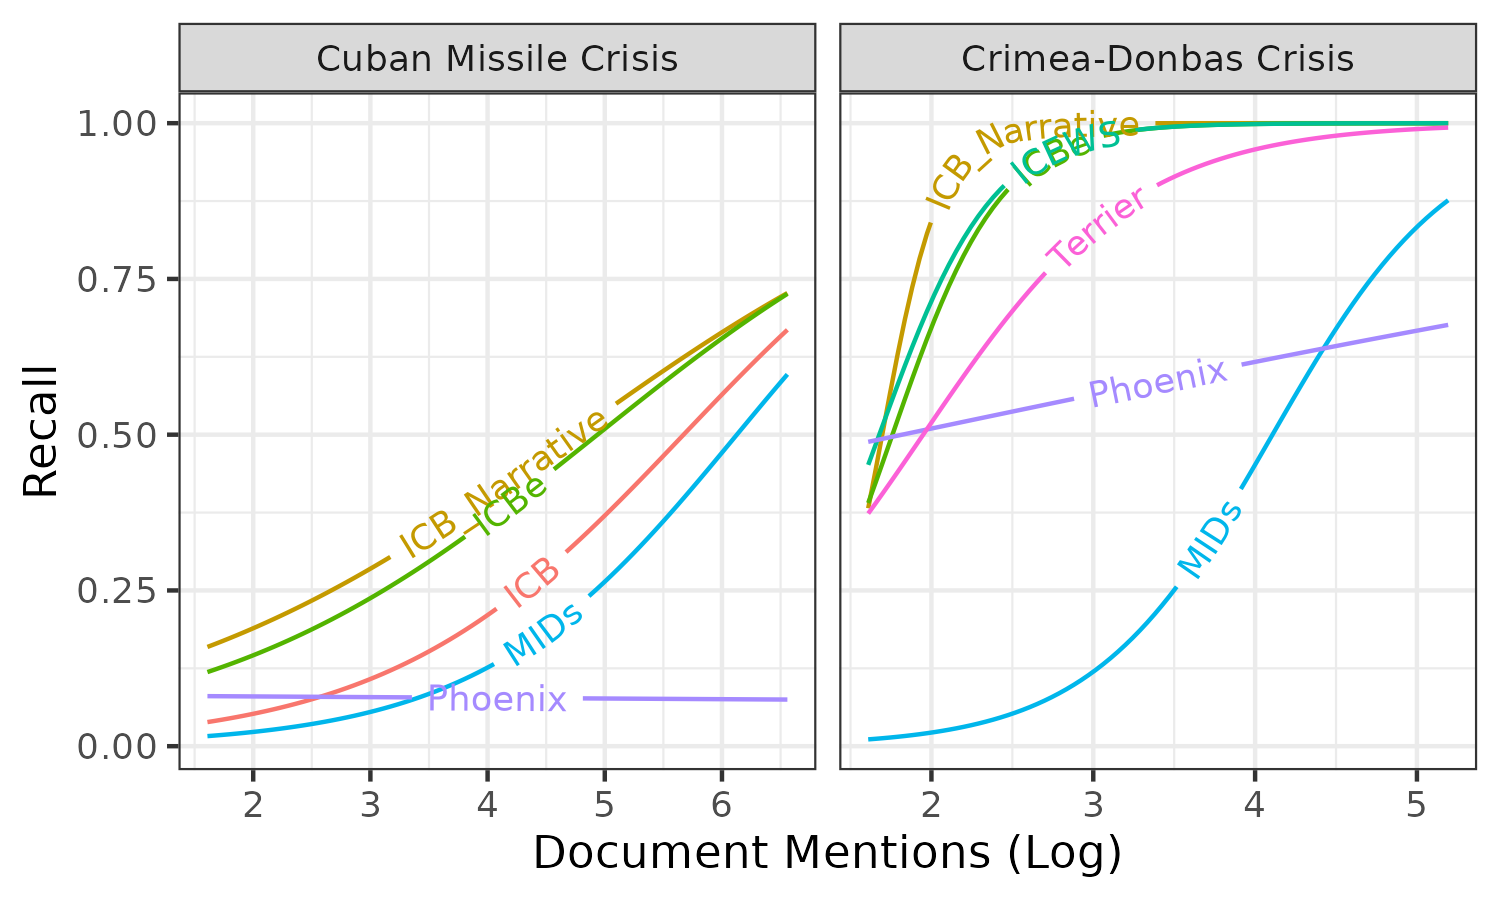
\includegraphics{p_recall.png}
\caption{Recall comparison of two cases across existing state of the art
efforts. Higher y-axis values represent higher recall and higher x-axis
values represent number of times that detail is mentioned across the
full corpus used to construct the synthetic
narrative.}\label{fig-recall-cases}
}
\end{figure}

The second component of event measurement validation is precision. It
does little good to recall a historical event but too vaguely (e.g.~MIDs
describes the Cuban Missile Crisis as a blockade, a show of force, and a
stalemate) or with too much error to be useful for downstream
applications (e.g.~ICEWS records 263 ``Detonate Nuclear Weapons'' events
between 1995-2019). ICBe's ontology and coding system are designed to
strike a balance so that the most important information is recovered
accurately but also abstracted to a level that is still useful and
interpretable.

How does ICBe's precision compare to the existing state of the art? A
researcher should be able to lay out the events of a crisis on a
timeline and read off the macrostructure of an episode from each
individual move. We call this visualization a crisis map, a directed
graph intersected with a timeline. A crisis map using ICBe for the Cuban
Missile Crisis case study is provided in Figure 2, and crisis maps for
the two case studies using existing event datasets can be found in SI
Appendix 4.3 and 4.4 and crisis maps for all crises using all datasets
can be found on the companion website. The crisis maps reveal the
episode-level datasets like MIDs or the original ICB are too sparse and
vague to reconstruct the structure of the crisis (SI Appendix 4.3 and
4.4). On the other end of the spectrum, the high recall dictionary-based
event datasets like Terrier and ICEWs produce so many noisy events
(several hundred thousand) that even with heavy filtering their crisis
maps are completely unintelligible. Further, because of copyright
issues, none of these datasets directly provide the original text spans
making event-level precision difficult to verify.

We further want to verify individual event codings, which we can do in
the case of ICBe because each event is mapped to a specific span of
text. We develop the iconography system for presenting event codings as
coherent statements that can be compared side by side to the original
source narrative for every case on the companion website. We further
provide a stratified sample of event codings alongside their source text
(SI Appendix 4.2). We find both the visualizations of macrostructure and
head-to-head comparisons of ICBe codings to the raw text to strongly
support the quality of ICBe.

Figure 3 shows the location of every sentence from the ICBe corpus in
semantic space as embedded using the same large language model as
before, and the median location of each ICBe event tag applied to those
sentences.\footnote{We preprocess sentences to replace named entities
  with a generic Entity token.} Labels reflect the individual leaves of
the ontology and colors reflect the higher level coarse branch nodes of
the ontology. If ICBe has high precision, substantively similar tags
ought to have been applied to substantively similar source text, which
is what we see both in two dimensions in the main plot and via
hierarchical clustering on all dimensions in the dendrogram along the
right-hand side.\footnote{Hierarchical clustering on cosine similarity
  and with Ward's method.}

\begin{figure}
\hypertarget{fig-umap}{%
\centering
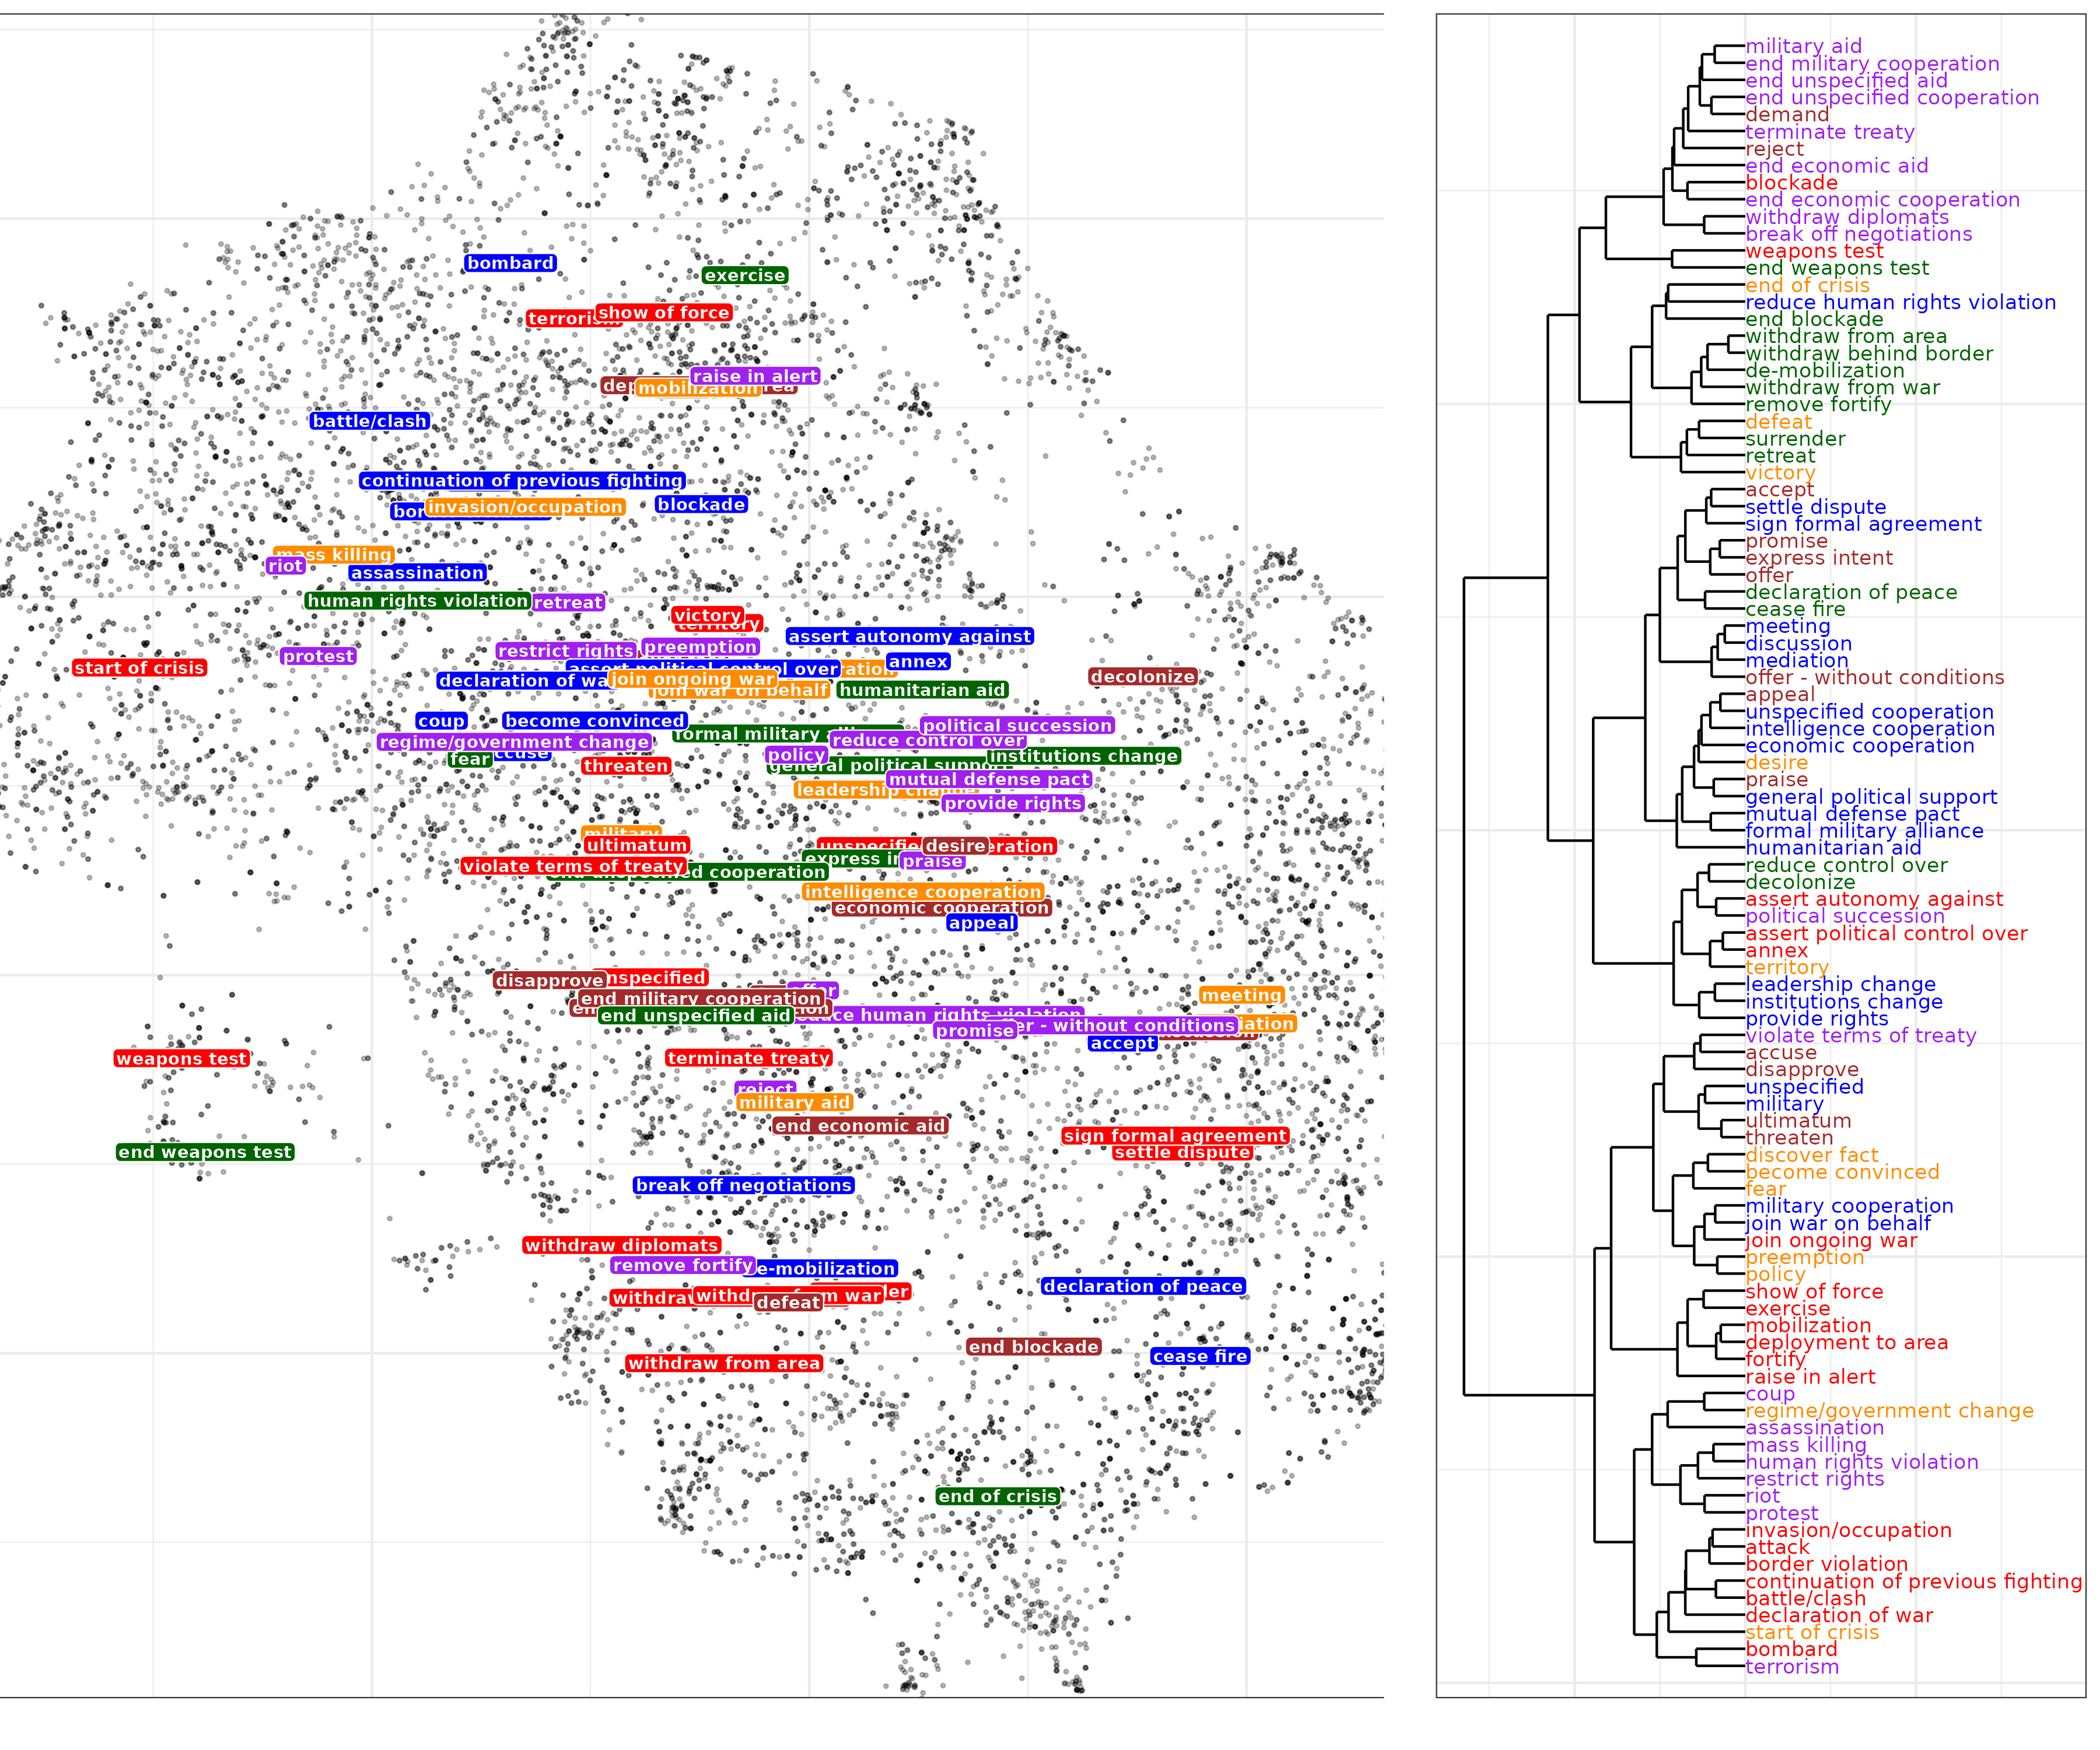
\includegraphics[width=7in,height=7in]{p_semantic_embeddings_dendro.png}
\caption{Dots represent individual ICB narrative sentences, as embedded
by the Paraphrase-MPNET-base-v2 large language model and flattened into
two dimensions with UMAP. Text labels reflect individual leaves of the
ICBe ontology, and colors represent intermediate branches of the
ontology. Label placement is the median of all of the sentences that the
tag was applied to by the coders. The dendrogram shows hierarchical
clustering of the tags. If ICBe precision is high, then the sentences
that tags were applied to ought to say similar things and the intended
shape of the ontology ought to be visually
recognizable.}\label{fig-umap}
}
\end{figure}

\hypertarget{case-illustrations}{%
\section{Case illustrations}\label{case-illustrations}}

In this section, we focus our validation on two case studies for which
we have produced synthetic narratives using the method described in
Section 3.2. Our proposed measure is a reconstruction task to see
whether our intended ontology can be recovered through only unsupervised
clustering of sentences they were applied to. The first (Figure 1) is
the Cuban Missile Crisis (hereafter Cuban Missiles) which took place
primarily in the second half of 1962, involved the United States, the
Soviet Union, and Cuba, and is widely known for bringing the world to
the brink of nuclear war. The second (SI Appendix 4.1) is the
Crimea-Donbas Crisis (hereafter Crimea-Donbas) which took place
primarily in 2014, involved Russia, Ukraine, and NATO, and within a
decade spiraled into a full-scale invasion. We choose these cases
because they are significant in contemporary international relations,
are widely known across academic disciplines as well as among the
public, and are sufficiently brief to evaluate in depth. They are
similar in that both cases involve a superpower in crisis with a
neighbor that changed from a friendly to a hostile regime, both held
implications for the economic and military security for the superpower
by risking full-scale invasion, and both eventually invited intervention
by an opposing superpower.

\hypertarget{cuban-missile-crisis-1962}{%
\subsection{Cuban Missile Crisis
(1962)}\label{cuban-missile-crisis-1962}}

A synthetic historical narrative for Cuban Missiles appears in Figure 4,
with 51 events drawn from 2,020 documents. Each row represents a detail
that appeared in at least five documents along with an approximate start
date, a handwritten summary, the number of documents it was mentioned
in, and whether it could be identified in the text of the original ICB
corpus, our ICBe events, and any of the competing existing models.

ICB's improved recall of Cuban Missiles was relative to the state of the
art was summarized in Section 3.2 (Figure 2), but the events that
explain that improvement can now be seen. Our ground truth ICB narrative
contains 17/51 of the events from the synthetic narrative of a case that
includes high-level previously classified details. ICBe captures nearly
all details included in ICB as well as more details from the synthetic
narrative than any competing dataset. Phoenix includes some earlier
information than ICBe like the nationalization of businesses and back
channel negotiations, but the crisis narrative has a clean canonical end
with the Soviets agreeing to withdraw missiles. ICBe stands out in
including more communicative behavior (do -- speech) than existing
datasets like US threats to attack and later promises not to invade.
Given the recognized importance of threat credibility for understanding
international conflict, the addition of this information is a
substantively important improvement over the existing state of the art
(Slantchev 2011).

\begin{figure}
\hypertarget{fig-recall-cuba}{%
\centering
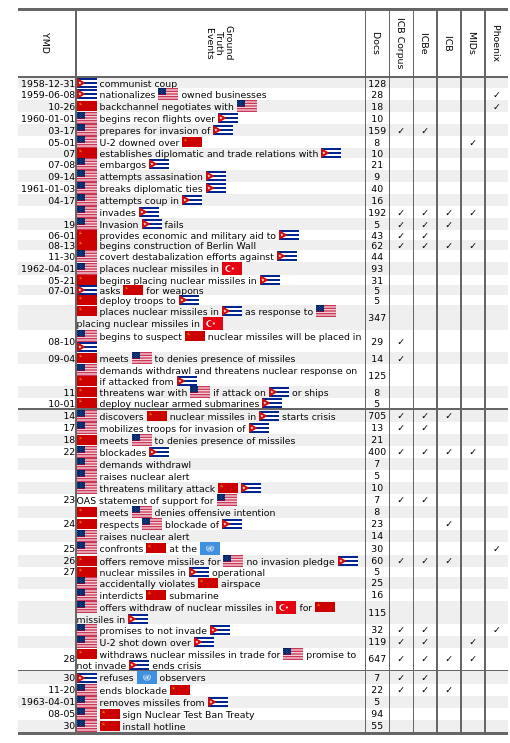
\includegraphics{case_study_cuban_recall.png}
\caption{Synthetic narratives combine several thousand accounts of each
crisis into a single timeline of events, taking only those mentioned in
at least 5 or more documents. Checkmarks represent whether that event
could be hand matched to any detail in the ICB corpus, ICBe dataset, or
any of the other event datasets (SI Appendix 3.2 and
3.3).}\label{fig-recall-cuba}
}
\end{figure}

Figure 5 shows the crisis map for the Cuban Missile Crisis. Looking at
the crisis on a timeline, one can now identify the structure of actors
and the environment, along with its supporting details, in a way that
validates the precision of ICBe. Although harder to measure objectively,
this crisis map provides face valid evidence that ICBe's account is not
too vague, but also not unnecessarily detailed. We include much of the
geopolitically important details like Soviet deployment, US discovery of
that deployment, heightened alert levels, a blockade, and negotiations
that ended with a formal agreement. At the same time, the crisis map
indicates that ICBe does not include unnecessary nuances that preclude
useful comparison to other international events.

\begin{figure}
\hypertarget{fig-cuba-crisismap}{%
\centering
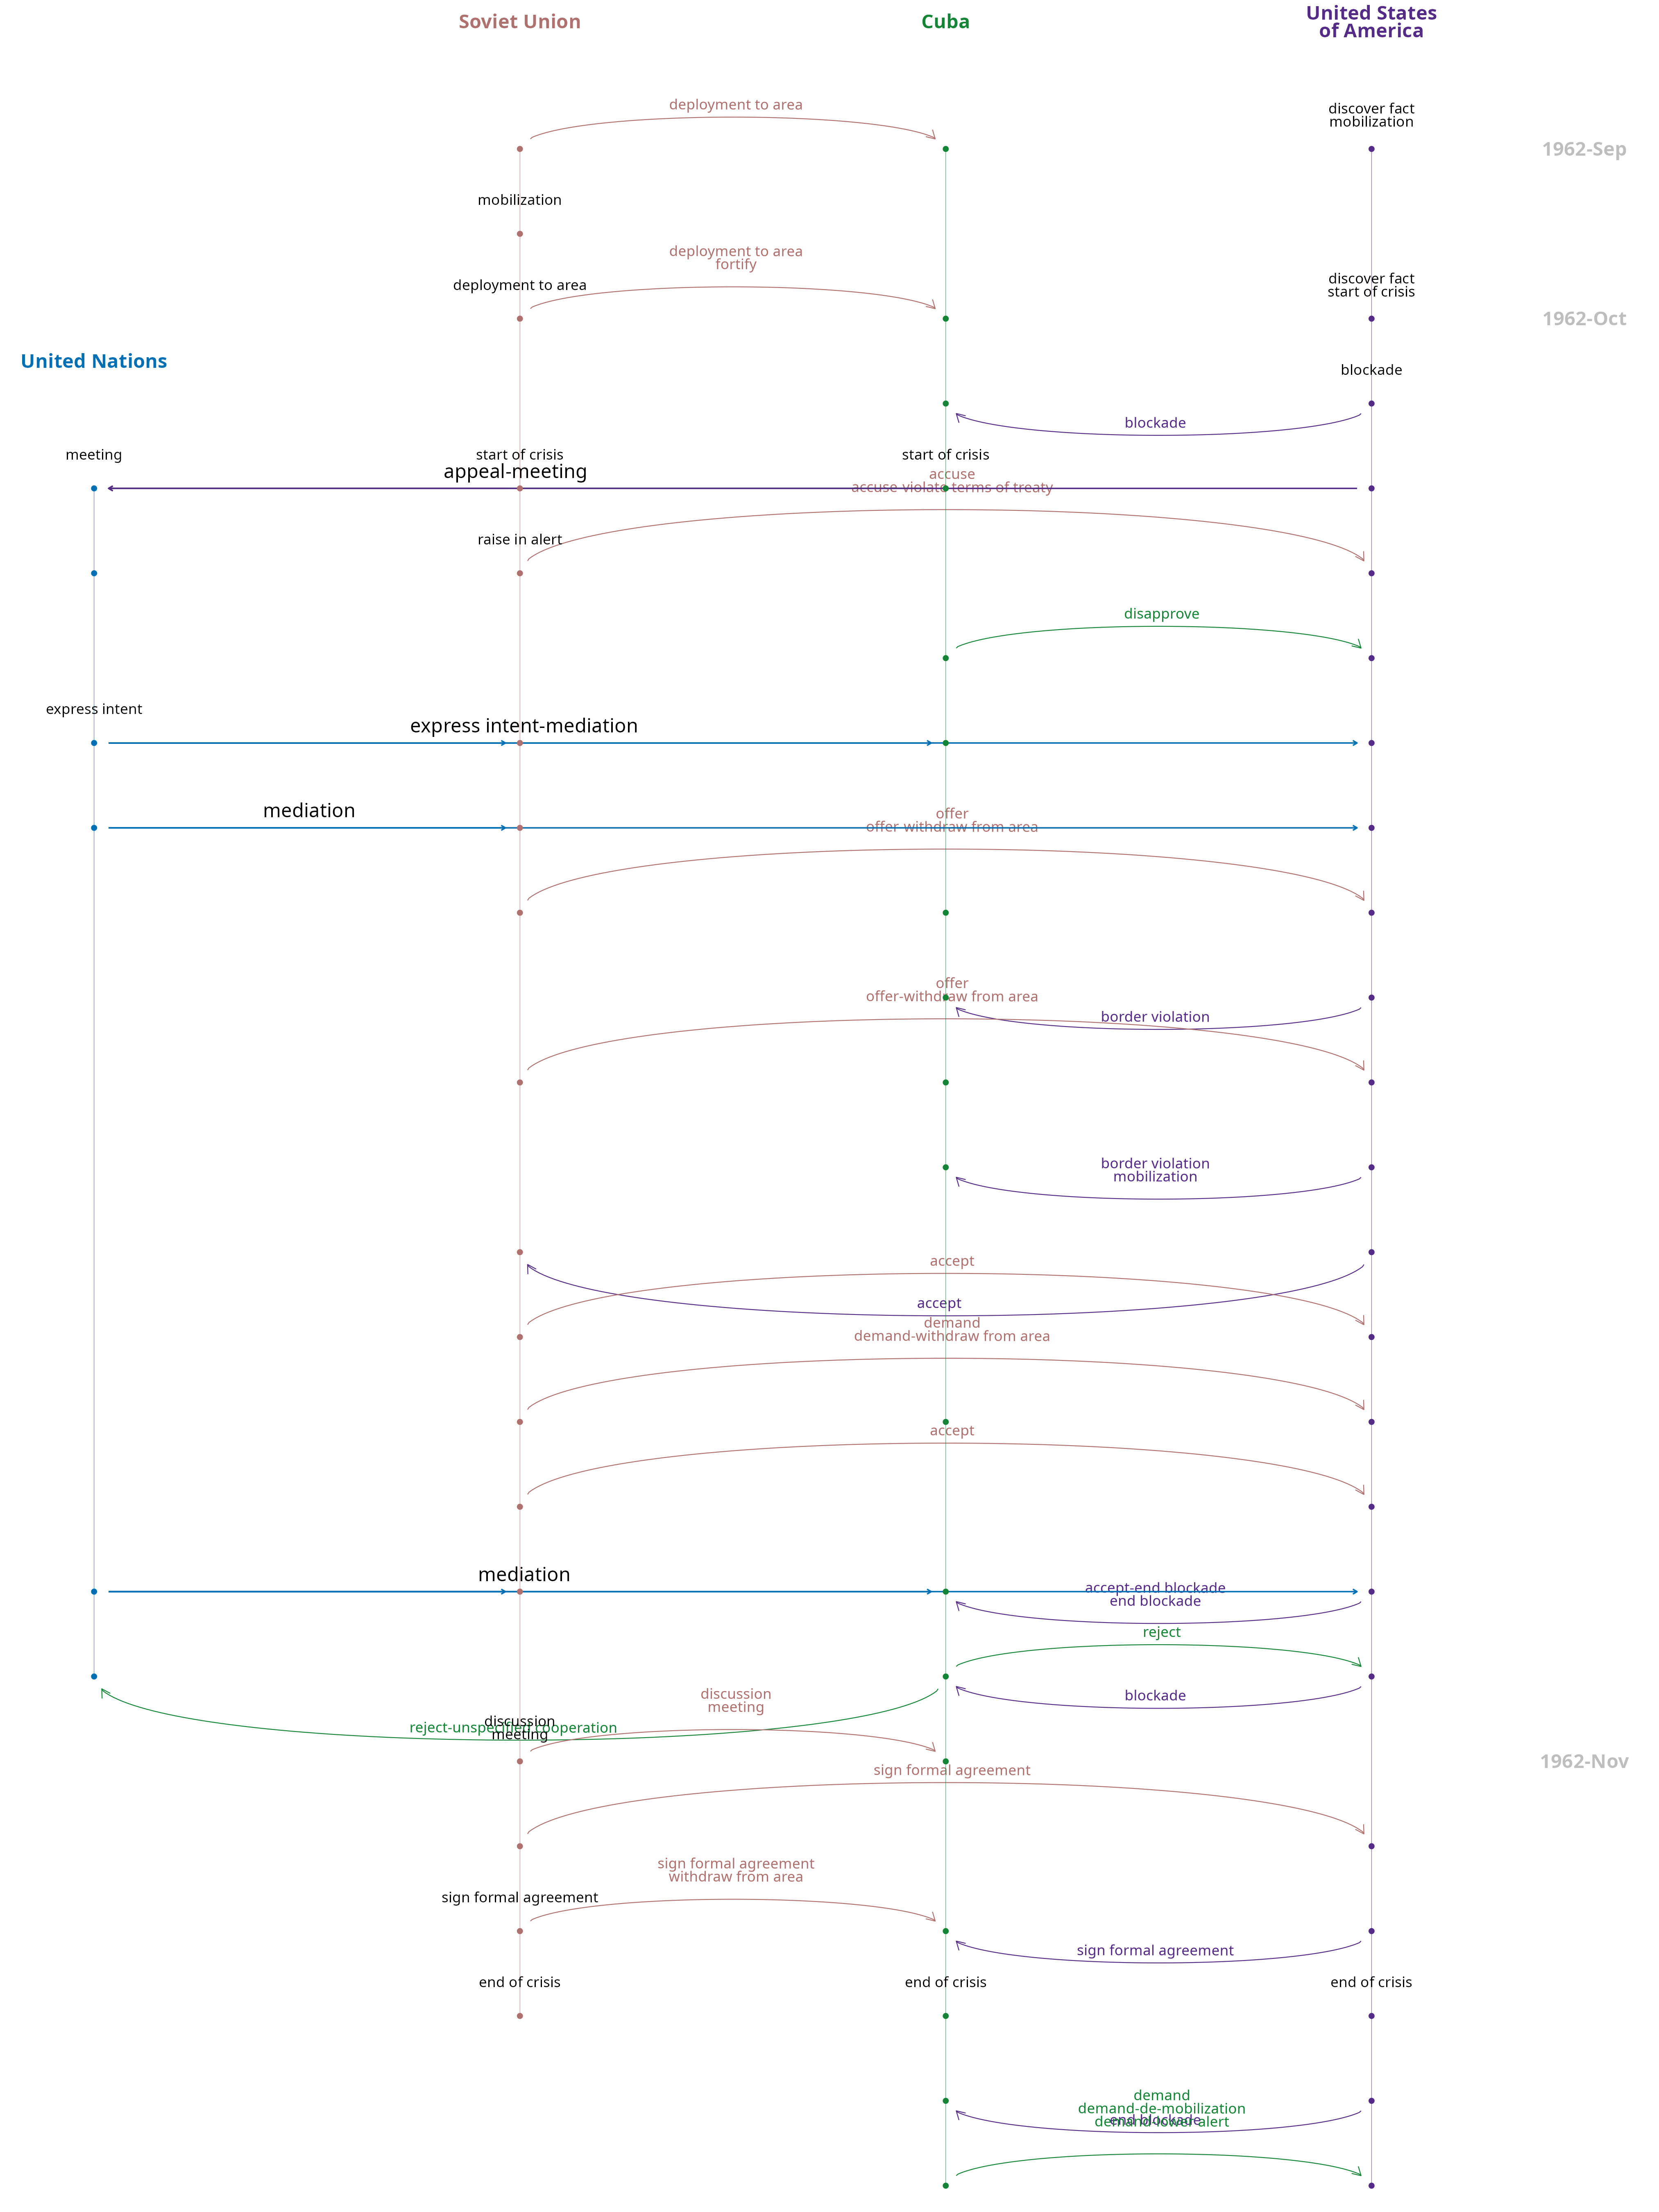
\includegraphics[width=6in,height=\textheight]{p_196_icbe.png}
\caption{Crisis map for the Cuban Missile Crisis. The start of the
crisis is at the top and end of the crisis is the bottom, with each
actor in a column with labeled points identifying their speeches,
actions, and thoughts.}\label{fig-cuba-crisismap}
}
\end{figure}

\hypertarget{crimea-donbas-2014}{%
\subsection{Crimea-Donbas (2014)}\label{crimea-donbas-2014}}

A synthetic historical narrative for the 2014 Crimea-Donbas crisis (30
events drawn from 971 documents) appears in Figure 6. As in the earlier
case, rows represent details that appeared in at least five documents
and whether it is identified in ICBe and existing datasets.

Again quantitatively summarized earlier in Section 3.2 (Figure 2), our
ground truth ICB narrative contains 23/30 of the events from the
synthetic narrative. Like the gray zone precursor to the Cuban Missile
crisis (Cormac and Aldrich 2018), Ukraine provided several security
guarantees to Russia that were potentially undone, e.g.~a long term
lease on naval facilities in Crimea. But unlike the Cuban Missile
crisis, the end of this crisis is unclear, with the event meekly ending
with a second cease-fire agreement (Minsk II) but continued fighting.
ICBe again recalls more important information about the crisis than any
existing dataset, particularly information concerning the behavior of
non-state separatist groups like the Donetsk People's Republic (DPR) and
Luhansk People's Republic (LPR).

\begin{figure}
\hypertarget{fig-recall-crimea}{%
\centering
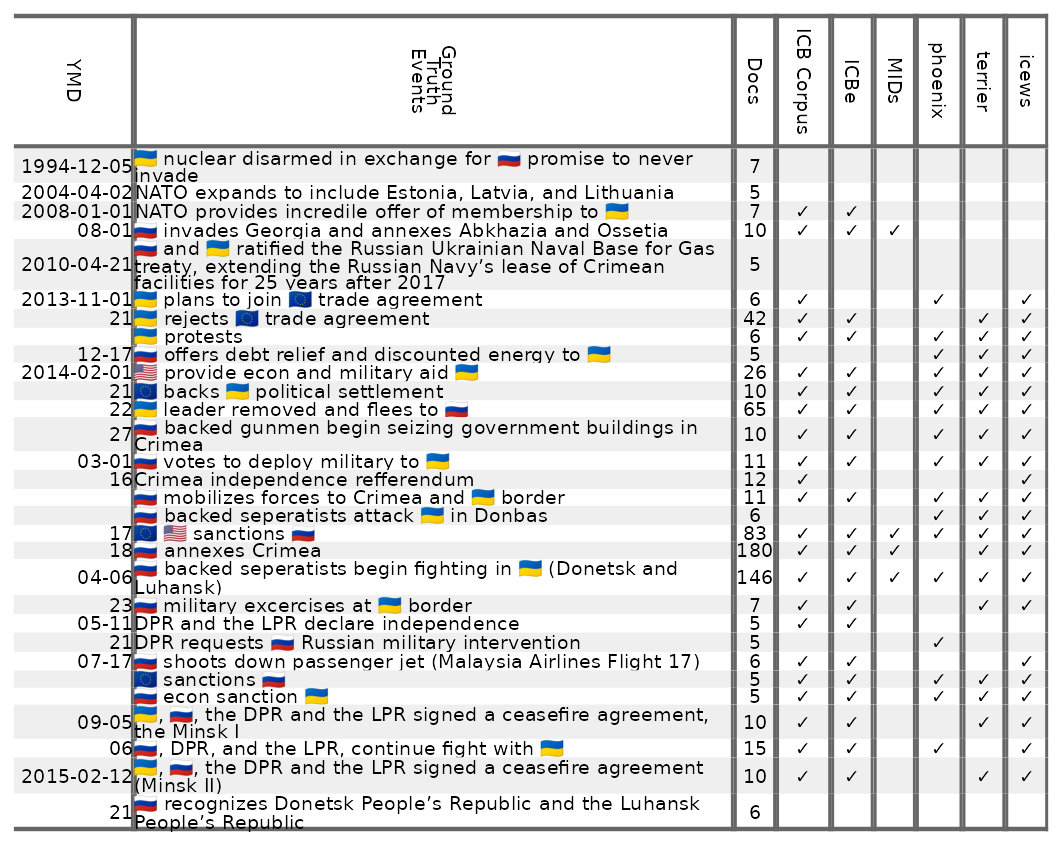
\includegraphics{case_study_crimea_recall.png}
\caption{Synthetic narratives combine several thousand accounts of each
crisis into a single timeline of events, taking only those mentioned in
at least 5 or more documents. Checkmarks represent whether that event
could be hand matched to any detail in the ICB corpus, ICBe dataset, or
any of the other event datasets (SI Appendix 3.2 and
3.3).}\label{fig-recall-crimea}
}
\end{figure}

As this more recent case reflects primarily public reporting rather than
the previously classified details relevant for the Cuban Missile Crisis,
ICBe's improvement relative to the global and real-time coverage of
dictionary-based event systems is still present, but less pronounced. We
want to take seriously the possibility that some functional
transformation could recover the precision of ICBe. For example,
Terechshenko (2020) attempts to correct for the mechanically increasing
amount of news coverage each year by de-trending violent event counts
from Phoenix using a human-coded baseline. Others have focused on
verifying precision for ICEWs on specific subsets of details against
known ground truths, e.g.~geolocation (Cook and Weidmann 2019), protest
events (80\%) (Wüest and Lorenzini 2020), anti-government protest
networks (46.1\%) (Jäger 2018).

We take the same approach here in Figure 7, selecting four specific
CAMEO event codings and checking how often they reflect a true
real-world event from the Crimea-Donbas synthetic narrative. We choose
four event types around key moments in the crisis. The start of the
crisis revolves around Ukraine backing out of a trade deal with the EU
in favor of Russia, but ``sign formal agreement'' events act more like a
topic detector with dozens of events generated by discussions of a
possible agreement but not the actual agreement which never
materialized. The switch is caught by the ``reject plan, agreement to
settle dispute'', but also continues for Viktor Yanukovych even after he
was removed from power because of articles retroactively discussing the
cause of his removal. Events for ``use conventional military force''
capture a threshold around the start of hostilities and who the
participants were but not any particular battles or campaigns. Likewise,
``impose embargo, boycott, or sanctions'' captures the start of waves of
sanctions and from who but are effectively constant as the news coverage
does not distinguish between subtle changes or additions. In sum,
dictionary-based methods on news corpora tend to have high recall
because they parse everything in the news, but for the same reason,
their specificity for most event types is too low to back out individual
chess-like sequencing that ICBe aims to record.

\begin{figure}
\hypertarget{fig-precision-icews}{%
\centering
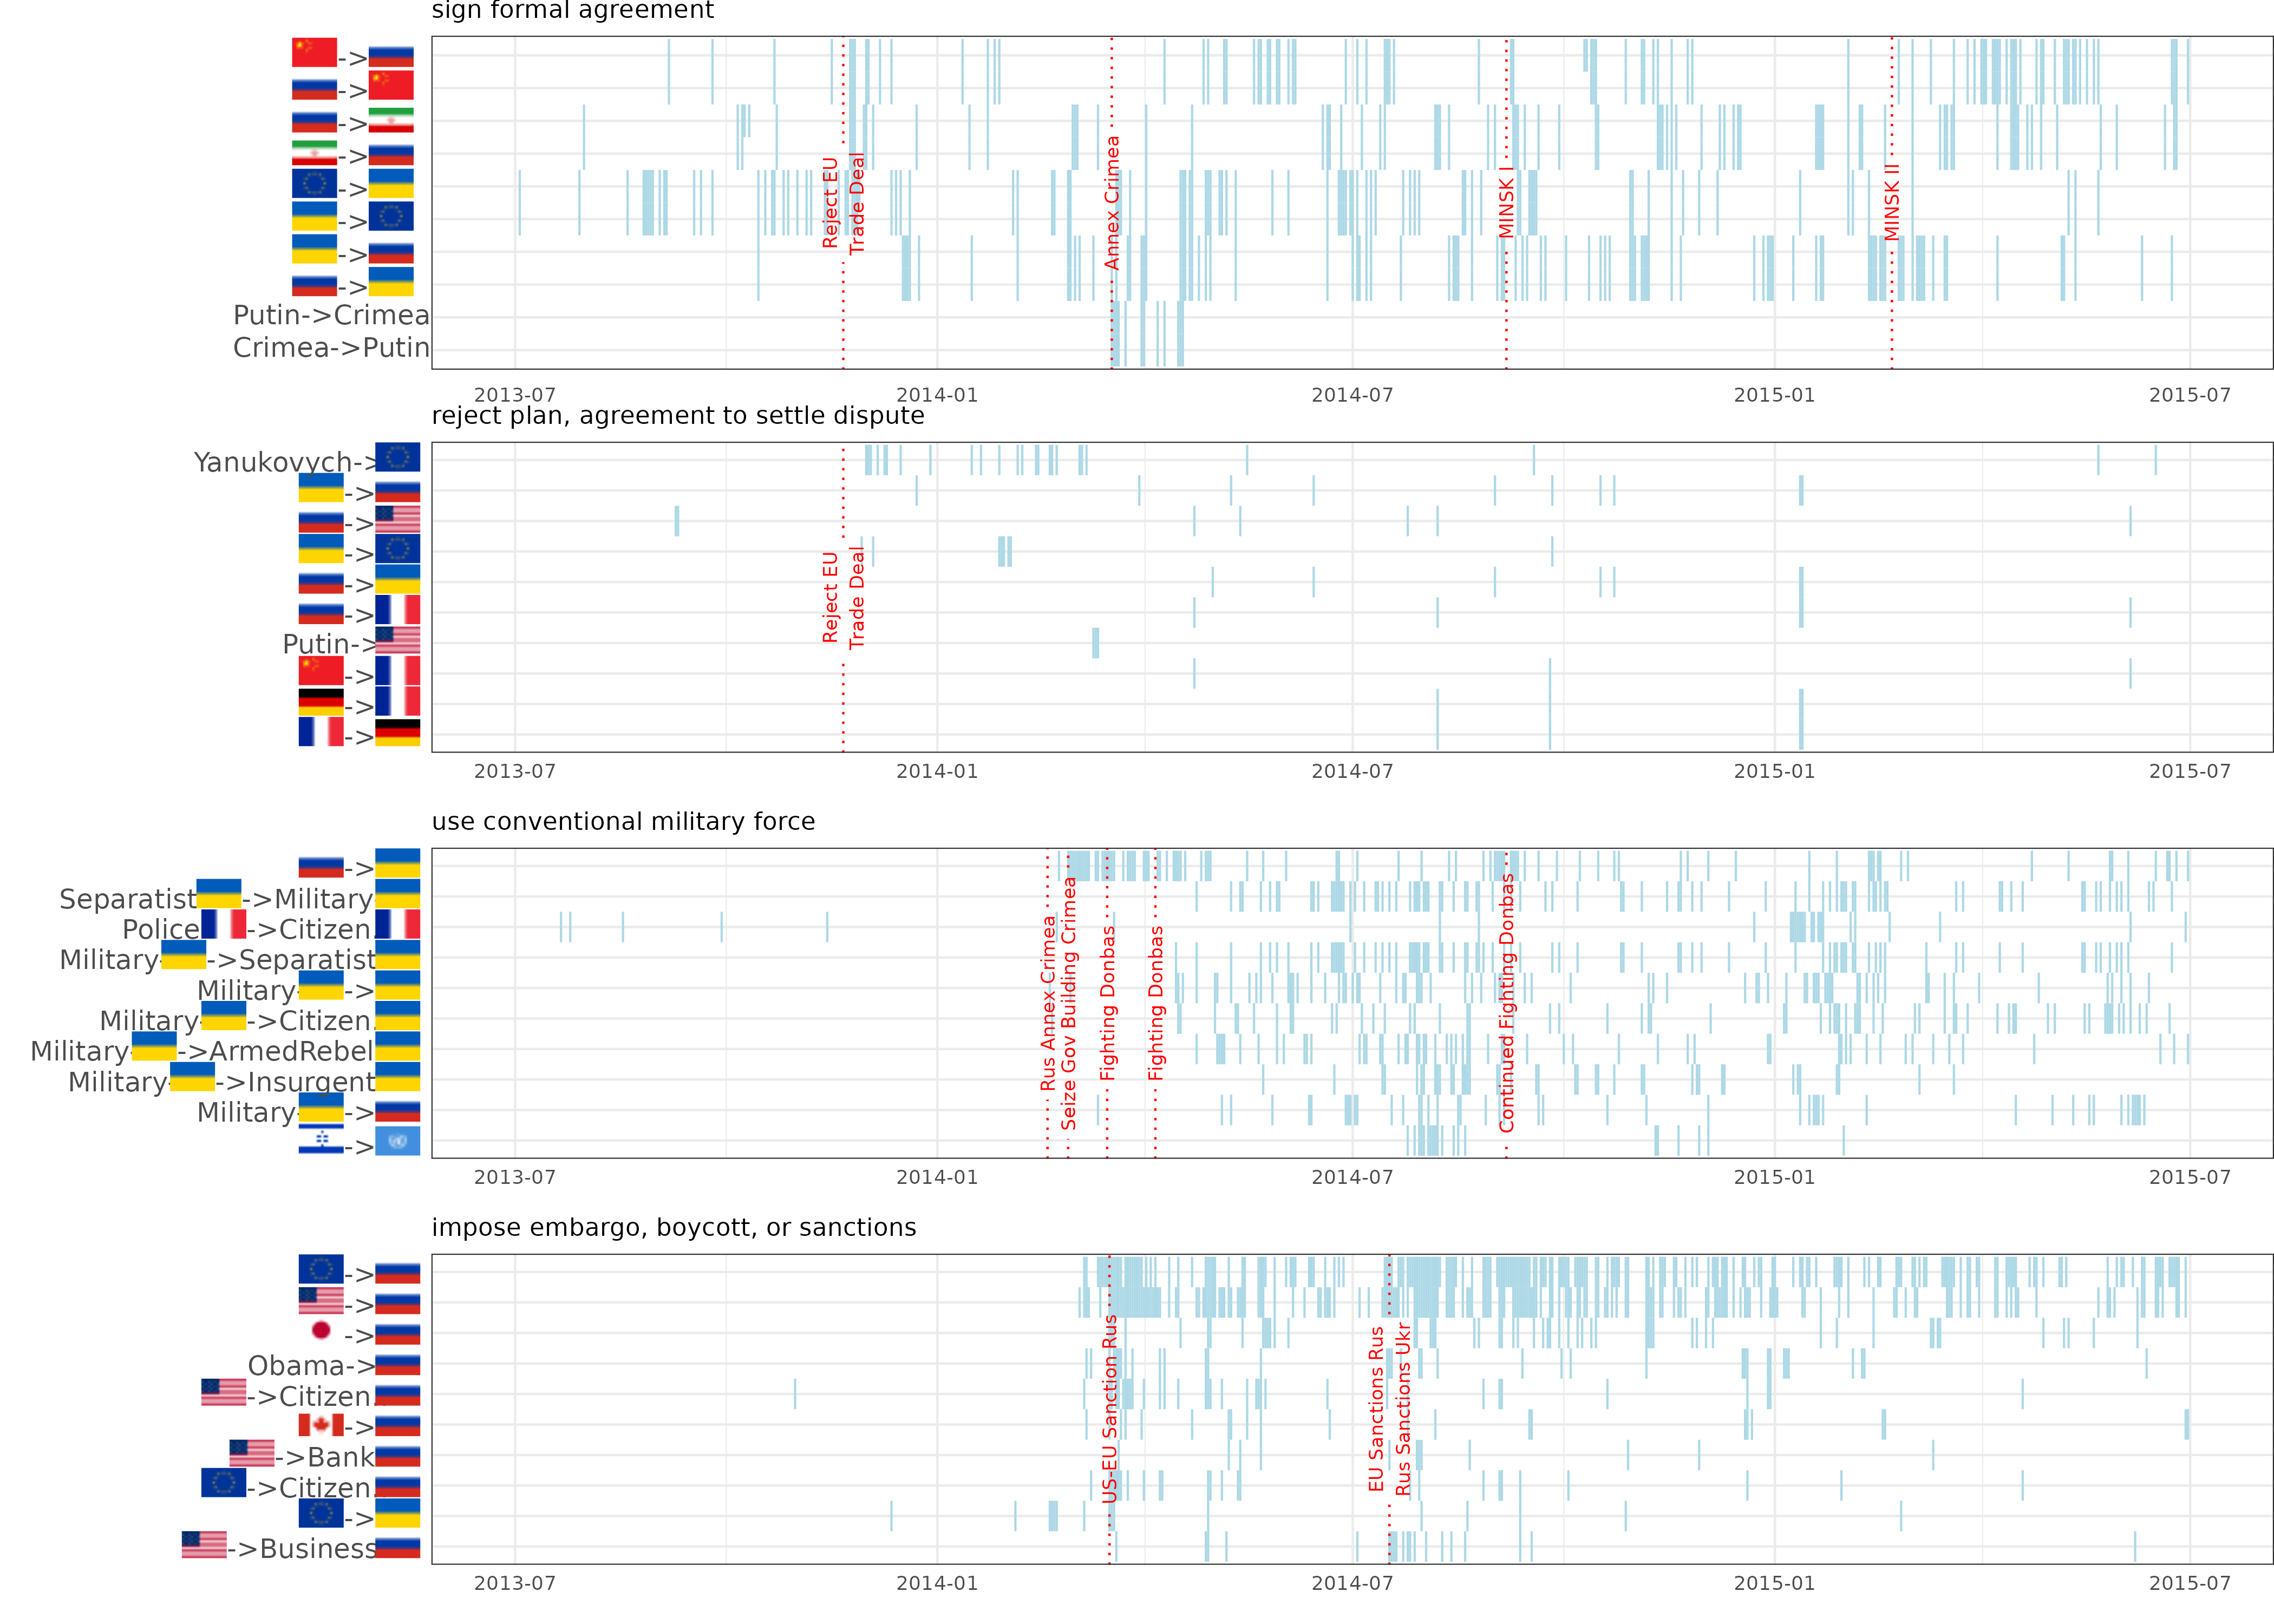
\includegraphics[width=7in,height=5in]{p_precision_icews.png}
\caption{The unit of analysis is the dyad-day. Top 10 most active dyads
per category shown. Red text shows events from the synthetic narrative
relative to that event category. Blue bars indicate an event recorded by
ICEWs for that dyad on that day.}\label{fig-precision-icews}
}
\end{figure}

\hypertarget{conclusion}{%
\section{Conclusion}\label{conclusion}}

We investigated event abstraction from narratives describing key
historical episodes in international relations. We synthesized a prior
belief about the latent unobserved phenomena that drive these events in
international relations and proposed a mapping to observable concepts
that enter into the observed historical record. We designed an ontology
with high coverage over those concepts and developed a training
procedure and technical stack for human coding of historical texts.
Multiple validity checks find the resulting codings have high internal
validity (e.g.~intercoder agreement) and external validity
(i.e.~matching source material in both micro-details at the sentence
level and macro-details spanning full historical episodes). Further,
these codings perform much better in terms of recall, precision,
coverage, and overall coherence in capturing these historical episodes
than existing event systems used in international relations.

We release several open-source products along with supporting code and
documentation to further advance the study of international relations,
event extraction, and natural language processing. The first is the
International Crisis Behavior Events (ICBe) dataset, an event-level
aggregation of what took place during the crises identified by the ICB
project. These data are appropriate for statistical analysis of hard
questions about the sequencing of events (e.g.~escalation and
de-escalation of conflicts).\footnote{Using ICBe data, Gannon (2022)
  finds that cross-domain crises are shorter and less violent than
  same-domain crises.} Second, we provide a coder-level disaggregation
with multiple codings of each sentence by experts and undergrads that
allows for the introduction of uncertainty and human interpretation of
events. Further, we release a direct mapping from the codings to the
source text at the sentence level as a new resource for natural language
processing. Finally, we provide a companion website that incorporates
detailed visualizations of all of the data introduced here at
crisisevents.org.

\hypertarget{funding}{%
\section{Funding}\label{funding}}

This work was supported by a grant from the Office of Naval Research
\(N00014-19-1-2491\) and from the Charles Koch Foundation \(20180481\).
The financial sponsors played no in the design, execution, analysis and
interpretation of data, or writing of the study.

\hypertarget{acknowledgements}{%
\section{Acknowledgements}\label{acknowledgements}}

We thank the ICB Project and its directors and contributors for their
foundational work and their help with this effort. We make special
acknowledgement of Michael Brecher for helping found the ICB project in
1975, creating a resource that continues to spark new insights to this
day. We thank the many undergraduate coders. Thanks to the Center for
Peace and Security Studies and its membership for comments. Special
thanks to Rebecca Cordell, Philip Schrodt, Zachary Steinert-Threlkeld,
and Zhanna Terechshenko for their generous feedback. Thank you to the
cPASS research assistants: Helen Chung, Daman Heer, Syeda ShahBano Ijaz,
Anthony Limon, Erin Ling, Ari Michelson, Prithviraj Pahwa, Gianna Pedro,
Tobias Stodiek, Yiyi `Effie' Sun, Erin Werner, Lisa Yen, and Ruixuan
Zhang.

\hypertarget{author-contributions}{%
\section{Author Contributions}\label{author-contributions}}

Conceptualization: R.W.D., E.G., J.L.; Methodology: R.W.D., T.L.S.;
Software: R.W.D.; Validation: R.W.D., T.L.S.; Formal Analysis: R.W.D.,
T.L.S.; Investigation: S.C., R.W.D., J.A.G., C.K., N.L., E.M., J.M.C.N.,
D.P., D.Q., J.W.; Data Curation: R.W.D., D.Q., T.L.S., J.W.; Writing -
Original Draft: R.W.D., T.L.S.; Writing - Review \& Editing: R.W.D.,
J.A.G., E.G., T.L.S.; Visualization: R.W.D., T.L.S.; Supervision: E.G.;
Project Administration: S.C., R.W.D., J.A.G., D.Q., T.L.S., J.W.;
Funding Acquisition: E.G., J.L.

\hypertarget{data-availability-statement}{%
\section{Data Availability
Statement}\label{data-availability-statement}}

This article's data, supplementary appendix, replication material, and
visualizations of every historical episode are available on the GitHub
repository
\href{https://urldefense.com/v3/__https://github.com/CenterForPeaceAndSecurityStudies/ICBEventData__;!!Mih3wA!WxDJtEczKfxGTh0S2Krunap8ReymFEL5iTWaSfOHeqlSdyfRx77zmjBSWO1OAm13$}{ICBEventData}
and through the companion website crisisevents.org.

\hypertarget{competing-interests-declaration}{%
\section{Competing Interests
Declaration}\label{competing-interests-declaration}}

The authors declare that there are no competing interests.

\clearpage

\hypertarget{works-cited}{%
\section*{Works Cited}\label{works-cited}}
\addcontentsline{toc}{section}{Works Cited}

\hypertarget{refs}{}
\begin{CSLReferences}{1}{0}
\leavevmode\vadjust pre{\hypertarget{ref-allenUSGlobalMilitary2021}{}}%
Allen, Michael A, Michael E Flynn, and Carla Martinez Machain. 2021.
{``{US} Global Military Deployments, 1950\textendash 2020*.''}
\emph{Conflict Management and Peace Science}, July, 07388942211030885.
\url{https://doi.org/10.1177/07388942211030885}.

\leavevmode\vadjust pre{\hypertarget{ref-allisonEssenceDecisionExplaining1971}{}}%
Allison, Graham T., and Philip Zelikow. 1971. \emph{Essence of Decision:
{Explaining} the {Cuban} Missile Crisis}. Vol. 327. {Little, Brown
Boston}.

\leavevmode\vadjust pre{\hypertarget{ref-althausClineCenterHistorical2019}{}}%
Althaus, Scott, Joseph Bajjalieh, John F. Carter, Buddy Peyton, and Dan
A. Shalmon. 2019. {``Cline {Center Historical Phoenix Event Data
Variable Descriptions}.''} \emph{Cline Center Historical Phoenix Event
Data}.

\leavevmode\vadjust pre{\hypertarget{ref-balaliCOfEEComprehensiveOntology2021}{}}%
Balali, Ali, Masoud Asadpour, and Seyed Hossein Jafari. 2021.
{``{COfEE}: {A Comprehensive Ontology} for {Event Extraction} from
Text.''} {arXiv}. \url{https://doi.org/10.48550/arXiv.2107.10326}.

\leavevmode\vadjust pre{\hypertarget{ref-beardsleyMediationDilemma2011}{}}%
Beardsley, Kyle. 2011. \emph{The Mediation Dilemma}. {Cornell University
Press}.

\leavevmode\vadjust pre{\hypertarget{ref-beardsleyInternationalCrisisBehavior2020}{}}%
Beardsley, Kyle, Patrick James, Jonathan Wilkenfeld, and Michael
Brecher. 2020. {``The {International Crisis Behavior Project}.''}
\emph{Oxford Research Encyclopedia of Politics}.
https://oxfordre.com/politics/view/10.1093/acrefore/9780190228637.001.0001/acrefore-9780190228637-e-1638.
\url{https://doi.org/10.1093/acrefore/9780190228637.013.1638}.

\leavevmode\vadjust pre{\hypertarget{ref-begerReassessingRoleTheory2021}{}}%
Beger, Andreas, Richard K. Morgan, and Michael D. Ward. 2021.
{``Reassessing the {Role} of {Theory} and {Machine Learning} in
{Forecasting Civil Conflict}.''} \emph{Journal of Conflict Resolution}
65 (7-8): 1405--26. \url{https://doi.org/10.1177/0022002720982358}.

\leavevmode\vadjust pre{\hypertarget{ref-beielerGeneratingPoliticalEvent2016}{}}%
Beieler, John, Patrick T. Brandt, Andrew Halterman, Philip A. Schrodt,
Erin M. Simpson, and R. Michael Alvarez. 2016. {``Generating Political
Event Data in Near Real Time.''} In \emph{Computational Social Science},
98. {Cambridge University Press}.

\leavevmode\vadjust pre{\hypertarget{ref-benyehudaEthnicActorsInternational2006}{}}%
Ben-Yehuda, Hemda, and Meirav MishaliRam. 2006. {``Ethnic {Actors} and
{International Crises}: {Theory} and {Findings},
1918\textendash 2001.''} \emph{International Interactions} 32 (1):
49--78. \url{https://doi.org/10.1080/03050620600584435}.

\leavevmode\vadjust pre{\hypertarget{ref-bloomfieldCASCONIIIComputeraided1989}{}}%
Bloomfield, Lincoln P., and Allen Moulton. 1989. {``{CASCON III}:
{Computer-aided} System for Analysis of Local Conflicts.''} \emph{MIT
Center for International Studies, Cambridge}.

\leavevmode\vadjust pre{\hypertarget{ref-boscheeICEWSCodedEvent2015}{}}%
Boschee, Elizabeth, Jennifer Lautenschlager, Sean O'Brien, Steve
Shellman, James Starz, and Michael Ward. 2015. {``{ICEWS} Coded Event
Data.''} \emph{Harvard Dataverse} 12.

\leavevmode\vadjust pre{\hypertarget{ref-brandtPhoenixRealTimeEvent2018}{}}%
Brandt, Patrick T., Vito DOrazio, Jennifer Holmes, Latifur Khan, and
Vincent Ng. 2018. {``Phoenix {Real-Time Event Data}.''}

\leavevmode\vadjust pre{\hypertarget{ref-brecherInternationalStudiesTwentieth1999}{}}%
Brecher, Michael. 1999. {``International Studies in the Twentieth
Century and Beyond: {Flawed} Dichotomies, Synthesis, Cumulation: {ISA}
Presidential Address.''} \emph{International Studies Quarterly} 43 (2):
213--64.

\leavevmode\vadjust pre{\hypertarget{ref-brecherCrisesWorldPolitics1982}{}}%
Brecher, Michael, and Jonathan Wilkenfeld. 1982. {``Crises in {World
Politics}.''} \emph{World Politics} 34 (3): 380--417.
\url{https://doi.org/10.2307/2010324}.

\leavevmode\vadjust pre{\hypertarget{ref-brecher_study_1997}{}}%
---------. 1997. \emph{A {Study} of {Crisis}}. {University of Michigan
Press}.

\leavevmode\vadjust pre{\hypertarget{ref-brecherInternationalCrisisBehavior2021}{}}%
Brecher, Michael, Jonathan Wilkenfeld, Kyle C. Beardsley, Patrick James,
and David Quinn. 2021. {``International {Crisis Behavior Data
Codebook}.''} Codebook Version 14.

\leavevmode\vadjust pre{\hypertarget{ref-brustIntegratingDomainKnowledge2020}{}}%
Brust, Clemens-Alexander, and Joachim Denzler. 2020. {``Integrating
Domain Knowledge: Using Hierarchies to Improve Deep Classifiers.''}
\emph{arXiv:1811.07125 {[}Cs{]}}, January.
\url{https://arxiv.org/abs/1811.07125}.

\leavevmode\vadjust pre{\hypertarget{ref-bushDensityDeclineFounding2019}{}}%
Bush, Sarah Sunn, and Jennifer Hadden. 2019. {``Density and {Decline} in
the {Founding} of {International NGOs} in the {United States}.''}
\emph{International Studies Quarterly} 63 (4): 1133--46.
\url{https://doi.org/10.1093/isq/sqz061}.

\leavevmode\vadjust pre{\hypertarget{ref-carafanoMeasuringMilitaryPower2014}{}}%
Carafano, James Jay. 2014. {``Measuring {Military Power}.''}
\emph{Strategic Studies Quarterly} 8 (3): 11--18.
\url{https://www.jstor.org/stable/26270616}.

\leavevmode\vadjust pre{\hypertarget{ref-carterStrategyTerritorialConflict2010}{}}%
Carter, David B. 2010. {``The {Strategy} of {Territorial Conflict}.''}
\emph{American Journal of Political Science} 54 (4): 969--87.
\url{https://doi.org/10.1111/j.1540-5907.2010.00471.x}.

\leavevmode\vadjust pre{\hypertarget{ref-chenowethIntroducingNonviolentAction2019}{}}%
Chenoweth, Erica, Cullen S Hendrix, and Kyleanne Hunter. 2019.
{``Introducing the {Nonviolent Action} in {Violent Contexts} ({NVAVC})
Dataset.''} \emph{Journal of Peace Research} 56 (2): 295--305.
\url{https://doi.org/10.1177/0022343318804855}.

\leavevmode\vadjust pre{\hypertarget{ref-cookLostAggregationImproving2019}{}}%
Cook, Scott J., and Nils B. Weidmann. 2019. {``Lost in {Aggregation}:
{Improving Event Analysis} with {Report-Level Data}.''} \emph{American
Journal of Political Science} 63 (1): 250--64.
\url{https://doi.org/10.1111/ajps.12398}.

\leavevmode\vadjust pre{\hypertarget{ref-cormacGreyNewBlack2018}{}}%
Cormac, Rory, and Richard J. Aldrich. 2018. {``Grey Is the New Black:
Covert Action and Implausible Deniability.''} \emph{International
Affairs} 94 (3): 477--94. \url{https://doi.org/10.1093/ia/iiy067}.

\leavevmode\vadjust pre{\hypertarget{ref-daviesOrganizedViolence19892022}{}}%
Davies, Shawn, Therése Pettersson, and Magnus Öberg. 2022. {``Organized
Violence 1989\textendash 2021 and Drone Warfare.''} \emph{Journal of
Peace Research} 59 (4): 593--610.

\leavevmode\vadjust pre{\hypertarget{ref-eckOneSidedViolenceCivilians2007}{}}%
Eck, Kristine, and Lisa Hultman. 2007. {``One-{Sided Violence Against
Civilians} in {War}: {Insights} from {New Fatality Data}.''}
\emph{Journal of Peace Research} 44 (2): 233--46.
\url{https://doi.org/10.1177/0022343307075124}.

\leavevmode\vadjust pre{\hypertarget{ref-fazalStateDeathPolitics2011}{}}%
Fazal, Tanisha M. 2011. \emph{State {Death}: {The Politics} and
{Geography} of {Conquest}, {Occupation}, and {Annexation}}. \emph{State
Death}. {Princeton University Press}.
\url{https://doi.org/10.1515/9781400841448}.

\leavevmode\vadjust pre{\hypertarget{ref-felbermayrGlobalSanctionsData2020}{}}%
Felbermayr, Gabriel, Aleksandra Kirilakha, Constantinos Syropoulos,
Erdal Yalcin, and Yoto V. Yotov. 2020. {``The Global Sanctions Data
Base.''} \emph{European Economic Review} 129 (October): 103561.
\url{https://doi.org/10.1016/j.euroecorev.2020.103561}.

\leavevmode\vadjust pre{\hypertarget{ref-fortnaPeaceTime2018}{}}%
Fortna, Virginia Page. 2018. \emph{Peace Time}. {Princeton University
Press}.

\leavevmode\vadjust pre{\hypertarget{ref-frederickIssueCorrelatesWar2017}{}}%
Frederick, Bryan A, Paul R Hensel, and Christopher Macaulay. 2017.
{``The {Issue Correlates} of {War Territorial Claims Data},
1816\textendash 20011.''} \emph{Journal of Peace Research} 54 (1):
99--108. \url{https://doi.org/10.1177/0022343316676311}.

\leavevmode\vadjust pre{\hypertarget{ref-gannonOneIfLand2022}{}}%
Gannon, J Andrés. 2022. {``One If by {Land}, and {Two} If by {Sea}:
{Cross-Domain Contests} and the {Escalation} of {International
Crises}.''} \emph{International Studies Quarterly} 66 (4): sqac065.
\url{https://doi.org/10.1093/isq/sqac065}.

\leavevmode\vadjust pre{\hypertarget{ref-gannonShadowDeterrenceWhy2022}{}}%
Gannon, J Andrés, Erik Gartzke, Jon R. Lindsay, and Peter Schram. 2022.
{``The {Shadow} of {Deterrence}: {Why Capable Actors Engage} in
{Contests Short} of {War}.''} \emph{Journal of Conflict Resolution},
00220027231166345.

\leavevmode\vadjust pre{\hypertarget{ref-gartzkeCrossDomainDeterrenceStrategy2019}{}}%
Gartzke, Erik, and Jon R. Lindsay. 2019. \emph{Cross-{Domain
Deterrence}: {Strategy} in an {Era} of {Complexity}}. {Oxford University
Press}.

\leavevmode\vadjust pre{\hypertarget{ref-gavinHistorySecurityStudies2014}{}}%
Gavin, Francis J. 2014. {``History, {Security Studies}, and the {July
Crisis}.''} \emph{Journal of Strategic Studies} 37 (2): 319--31.
\url{https://doi.org/10.1080/01402390.2014.912916}.

\leavevmode\vadjust pre{\hypertarget{ref-giblerInternationalConflicts181620102018}{}}%
Gibler, Douglas M. 2018. \emph{International {Conflicts}, 1816-2010:
{Militarized Interstate Dispute Narratives}}. {Rowman \& Littlefield}.

\leavevmode\vadjust pre{\hypertarget{ref-giblerMeasuringAlliancesCorrelates2004}{}}%
Gibler, Douglas M., and Meredith Reid Sarkees. 2004. {``Measuring
{Alliances}: The {Correlates} of {War Formal Interstate Alliance}
{Dataset}, 1816\textendash 2000.''} \emph{Journal of Peace Research} 41
(2): 211--22. \url{https://doi.org/10.1177/0022343304041061}.

\leavevmode\vadjust pre{\hypertarget{ref-glaserCausesConsequencesArms2000}{}}%
Glaser, Charles L. 2000. {``The {Causes} and {Consequences} of {Arms
Races}.''} \emph{Annual Review of Political Science} 3 (1): 251--76.
\url{https://doi.org/10.1146/annurev.polisci.3.1.251}.

\leavevmode\vadjust pre{\hypertarget{ref-goemansIntroducingArchigosDataset2009}{}}%
Goemans, Henk E., Kristian Skrede Gleditsch, and Giacomo Chiozza. 2009.
{``Introducing {Archigos}: {A} Dataset of Political Leaders.''}
\emph{Journal of Peace Research} 46 (2): 269--83.

\leavevmode\vadjust pre{\hypertarget{ref-goertzMeasuringMilitaryAllocations1986}{}}%
Goertz, Gary, and Paul F. Diehl. 1986. {``Measuring {Military
Allocations}: {A Comparison} of {Different Approaches}.''} \emph{Journal
of Conflict Resolution} 30 (3): 553--81.
\url{https://doi.org/10.1177/0022002786030003009}.

\leavevmode\vadjust pre{\hypertarget{ref-goldgeierPsychologyInternationalRelations2001}{}}%
Goldgeier, J. M., and P. E. Tetlock. 2001. {``Psychology and
{International Relations Theory}.''} \emph{Annual Review of Political
Science} 4 (1): 67--92.
\url{https://doi.org/10.1146/annurev.polisci.4.1.67}.

\leavevmode\vadjust pre{\hypertarget{ref-grantOUEventData2017}{}}%
Grant, Christan, Andrew Halterman, Jill Irvine, Yan Liang, and Khaled
Jabr. 2017. {``{OU Event Data Project},''} December.

\leavevmode\vadjust pre{\hypertarget{ref-haffarEmergentPeacemakersCataloguing2002}{}}%
Haffar, Warren. 2002. {``Emergent {Peacemakers}: {Cataloguing New
Patterns} of {Activity} in {Post-Cold War Conflict}.''} \emph{Peace
Economics, Peace Science and Public Policy} 8 (2).
\url{https://doi.org/10.2202/1554-8597.1054}.

\leavevmode\vadjust pre{\hypertarget{ref-hermannComparativeResearchEvents1984}{}}%
Hermann, Charles. 1984. {``Comparative {Research} on the {Events} of
{Nations} ({CREON}) {Project}: {Foreign Policy Events}, 1959-1968:
{Version} 1.''} {ICPSR - Interuniversity Consortium for Political and
Social Research}. \url{https://doi.org/10.3886/ICPSR05205.V1}.

\leavevmode\vadjust pre{\hypertarget{ref-hewittEngagingInternationalData2001}{}}%
Hewitt, J. Joseph. 2001. {``Engaging {International Data} in the
{Classroom}: {Using} the {ICB Interactive Data Library} to {Teach
Conflict} and {Crisis Analysis}.''} \emph{International Studies
Perspectives} 2 (4): 371--83.
\url{https://doi.org/10.1111/1528-3577.00066}.

\leavevmode\vadjust pre{\hypertarget{ref-holsti1914Case1965}{}}%
Holsti, Ole R. 1965. {``The 1914 {Case}.''} \emph{The American Political
Science Review} 59 (2): 365--78. \url{https://doi.org/10.2307/1953055}.

\leavevmode\vadjust pre{\hypertarget{ref-hsuStatesHarnessingSubnational2020}{}}%
Hsu, Angel, Niklas Höhne, Takeshi Kuramochi, Virginia Vilariño, and
Benjamin K. Sovacool. 2020. {``Beyond States: {Harnessing} Sub-National
Actors for the Deep Decarbonisation of Cities, Regions, and
Businesses.''} \emph{Energy Research \& Social Science} 70 (December):
101738. \url{https://doi.org/10.1016/j.erss.2020.101738}.

\leavevmode\vadjust pre{\hypertarget{ref-iakhnisCrisesWorldPolitics2019}{}}%
Iakhnis, Evgeniia, and Patrick James. 2019. {``Near Crises in World
Politics: {A} New Dataset.''} \emph{Conflict Management and Peace
Science}, July, 0738894219855610.
\url{https://doi.org/10.1177/0738894219855610}.

\leavevmode\vadjust pre{\hypertarget{ref-jagerLimitsStudyingNetworks2018}{}}%
Jäger, Kai. 2018. {``The {Limits} of {Studying Networks} with {Event
Data}: {Evidence} from the {ICEWS Dataset}.''} \emph{Journal of Global
Security Studies} 3 (4): 498--511.

\leavevmode\vadjust pre{\hypertarget{ref-jervisCooperationSecurityDilemma1978}{}}%
Jervis, Robert. 1978. {``Cooperation {Under} the {Security Dilemma}.''}
\emph{World Politics} 30 (2): 167--214.
\url{https://doi.org/10.2307/2009958}.

\leavevmode\vadjust pre{\hypertarget{ref-kangUSBiasStudy2019}{}}%
Kang, David C., and Alex Yu-Ting Lin. 2019. {``{US} Bias in the Study of
{Asian} Security: {Using Europe} to Study {Asia}.''} \emph{Journal of
Global Security Studies} 4 (3): 393--401.

\leavevmode\vadjust pre{\hypertarget{ref-kinneDefenseCooperationAgreement2020}{}}%
Kinne, Brandon J. 2020. {``The {Defense Cooperation Agreement Dataset}
({DCAD}).''} \emph{Journal of Conflict Resolution} 64 (4): 729--55.
\url{https://doi.org/10.1177/0022002719857796}.

\leavevmode\vadjust pre{\hypertarget{ref-lacinaExplainingSeverityCivil2006}{}}%
Lacina, Bethany. 2006. {``Explaining the {Severity} of {Civil Wars}.''}
\emph{Journal of Conflict Resolution} 50 (2): 276--89.
\url{https://doi.org/10.1177/0022002705284828}.

\leavevmode\vadjust pre{\hypertarget{ref-lafreeIntroducingGlobalTerrorism2007}{}}%
LaFree, Gary, and Laura Dugan. 2007. {``Introducing the Global Terrorism
Database.''} \emph{Terrorism and Political Violence} 19 (2): 181--204.

\leavevmode\vadjust pre{\hypertarget{ref-laiEffectsDifferentTypes2004}{}}%
Lai, Brian. 2004. {``The Effects of Different Types of Military
Mobilization on the Outcome of International Crises.''} \emph{Journal of
Conflict Resolution} 48 (2): 211--29.

\leavevmode\vadjust pre{\hypertarget{ref-leedsDomesticPoliticalInstitutions1999}{}}%
Leeds, Brett Ashley. 1999. {``Domestic {Political Institutions},
{Credible Commitments}, and {International Cooperation}.''}
\emph{American Journal of Political Science} 43 (4): 979--1002.
\url{https://doi.org/10.2307/2991814}.

\leavevmode\vadjust pre{\hypertarget{ref-leedsAllianceReliabilityTimes2003}{}}%
---------. 2003. {``Alliance {Reliability} in {Times} of {War}:
{Explaining State Decisions} to {Violate Treaties}.''}
\emph{International Organization} 57 (4): 801--27.
\url{https://doi.org/10.1017/S0020818303574057}.

\leavevmode\vadjust pre{\hypertarget{ref-lengMilitarizedInterstateCrises1988}{}}%
Leng, Russell J., and J. David Singer. 1988. {``Militarized {Interstate
Crises}: {The BCOW Typology} and {Its Applications}.''}
\emph{International Studies Quarterly} 32 (2): 155--73.
\url{https://doi.org/10.2307/2600625}.

\leavevmode\vadjust pre{\hypertarget{ref-liComprehensiveSurveySchemabased2021}{}}%
Li, Qian, Hao Peng, Jianxin Li, Yiming Hei, Rui Sun, Jiawei Sheng, Shu
Guo, et al. 2021. {``A {Comprehensive Survey} on {Schema-based Event
Extraction} with {Deep Learning}.''} \emph{arXiv:2107.02126 {[}Cs{]}},
August. \url{https://arxiv.org/abs/2107.02126}.

\leavevmode\vadjust pre{\hypertarget{ref-lindsayPoliticsManyOther2020}{}}%
Lindsay, Jon R., and Erik Gartzke. 2020. {``Politics by Many Other
Means: {The} Comparative Strategic Advantages of Operational Domains.''}
\emph{Journal of Strategic Studies} 0 (0): 1--34.
\url{https://doi.org/10.1080/01402390.2020.1768372}.

\leavevmode\vadjust pre{\hypertarget{ref-luptonReexaminingReputationResolve2018}{}}%
Lupton, Danielle L. 2018. {``Reexamining {Reputation} for {Resolve}:
{Leaders}, {States}, and the {Onset} of {International Crises}.''}
\emph{Journal of Global Security Studies} 3 (2): 198--216.
\url{https://doi.org/10.1093/jogss/ogy004}.

\leavevmode\vadjust pre{\hypertarget{ref-mandelbrotFractalGeometryNature1983}{}}%
Mandelbrot, Benoit B. 1983. \emph{{The fractal geometry of nature}}.
{New York}: {Freeman}.

\leavevmode\vadjust pre{\hypertarget{ref-mcclellandWorldEventInteraction1978}{}}%
McClelland, Charles. 1978. {``World Event/Interaction Survey,
1966-1978.''} \emph{WEIS Codebook ICPSR} 5211.

\leavevmode\vadjust pre{\hypertarget{ref-mcnabbcochranMeasuringMilitaryEffectiveness2017}{}}%
McNabb Cochran, Kathryn, and Stephen B. Long. 2017. {``Measuring
{Military Effectiveness}: {Calculating Casualty Loss-Exchange Ratios}
for {Multilateral Wars}, 1816\textendash 1990.''} \emph{International
Interactions} 43 (6): 1019--40.
\url{https://doi.org/10.1080/03050629.2017.1273914}.

\leavevmode\vadjust pre{\hypertarget{ref-merrittMeasuringEventsInternational1994}{}}%
Merritt, Richard L. 1994. {``Measuring Events for International
Political Analysis.''} \emph{International Interactions} 20 (1-2):
3--33.

\leavevmode\vadjust pre{\hypertarget{ref-millerWordNetLexicalDatabase1995}{}}%
Miller, George A. 1995. {``{WordNet}: A Lexical Database for
{English}.''} \emph{Communications of the ACM} 38 (11): 39--41.
\url{https://doi.org/10.1145/219717.219748}.

\leavevmode\vadjust pre{\hypertarget{ref-minInterstateWarBattle2021}{}}%
Min, Eric. 2021. {``Interstate {War Battle} Dataset
(1823\textendash 2003).''} \emph{Journal of Peace Research} 58 (2):
294--303. \url{https://doi.org/10.1177/0022343320913305}.

\leavevmode\vadjust pre{\hypertarget{ref-moyerWhatAreDrivers2020}{}}%
Moyer, Jonathan D, Sara D Turner, and Collin J Meisel. 2020. {``What Are
the Drivers of Diplomacy? {Introducing} and Testing New Annual Dyadic
Data Measuring Diplomatic Exchange.''} \emph{Journal of Peace Research},
September, 0022343320929740.
\url{https://doi.org/10.1177/0022343320929740}.

\leavevmode\vadjust pre{\hypertarget{ref-narangCivilmilitaryPathologiesDefeat2017}{}}%
Narang, Vipin, and Caitlin Talmadge. 2017. {``Civil-Military
{Pathologies} and {Defeat} in {War}: {Tests Using New Data}.''}
\emph{Journal of Conflict Resolution}, January, 0022002716684627.
\url{https://doi.org/10.1177/0022002716684627}.

\leavevmode\vadjust pre{\hypertarget{ref-narayanDontGiveMe2018}{}}%
Narayan, Shashi, Shay B Cohen, and Mirella Lapata. 2018. {``Don't Give
Me the Details, Just the Summary! Topic-Aware Convolutional Neural
Networks for Extreme Summarization.''} \emph{arXiv Preprint
arXiv:1808.08745}.

\leavevmode\vadjust pre{\hypertarget{ref-oneillInternationalNegotiationConceptual2018}{}}%
O'Neill, Barry. 2018. {``International {Negotiation}: {Some Conceptual
Developments}.''} \emph{Annual Review of Political Science} 21 (1):
515--33. \url{https://doi.org/10.1146/annurev-polisci-031416-092909}.

\leavevmode\vadjust pre{\hypertarget{ref-owsiakInternationalBorderAgreements2018}{}}%
Owsiak, Andrew P, Allison K Cuttner, and Brent Buck. 2018. {``The
{International Border Agreements Dataset}.''} \emph{Conflict Management
and Peace Science} 35 (5): 559--76.
\url{https://doi.org/10.1177/0738894216646978}.

\leavevmode\vadjust pre{\hypertarget{ref-paigeKoreanDecisionJune1968}{}}%
Paige, Glenn D. 1968. \emph{The {Korean Decision}, {June} 24-30, 1950}.
{Free Press}.

\leavevmode\vadjust pre{\hypertarget{ref-palmerMID5Dataset20112021}{}}%
Palmer, Glenn, Roseanne W McManus, Vito D'Orazio, Michael R Kenwick,
Mikaela Karstens, Chase Bloch, Nick Dietrich, Kayla Kahn, Kellan Ritter,
and Michael J Soules. 2021. {``The {MID5 Dataset}, 2011\textendash 2014:
{Procedures}, Coding Rules, and Description.''} \emph{Conflict
Management and Peace Science}, February, 0738894221995743.
\url{https://doi.org/10.1177/0738894221995743}.

\leavevmode\vadjust pre{\hypertarget{ref-powellGlobalInstancesCoups2011}{}}%
Powell, Jonathan M, and Clayton L Thyne. 2011. {``Global Instances of
Coups from 1950 to 2010: {A} New Dataset.''} \emph{Journal of Peace
Research} 48 (2): 249--59.
\url{https://doi.org/10.1177/0022343310397436}.

\leavevmode\vadjust pre{\hypertarget{ref-powellBargainingTheoryInternational2002}{}}%
Powell, Robert. 2002. {``Bargaining {Theory} and {International
Conflict}.''} \emph{Annual Review of Political Science} 5 (1): 1--30.
\url{https://doi.org/10.1146/annurev.polisci.5.092601.141138}.

\leavevmode\vadjust pre{\hypertarget{ref-quinnPowerPlayMediation2006}{}}%
Quinn, David, Jonathan Wilkenfeld, Kathleen Smarick, and Victor Asal.
2006. {``Power {Play}: {Mediation} in {Symmetric} and {Asymmetric
International Crises}.''} \emph{International Interactions} 32 (4):
441--70. \url{https://doi.org/10.1080/03050620601011107}.

\leavevmode\vadjust pre{\hypertarget{ref-raleighIntroducingACLEDArmed2010}{}}%
Raleigh, Clionadh, Andrew Linke, Håavard Hegre, and Joakim Karlsen.
2010. {``Introducing {ACLED}: An Armed Conflict Location and Event
Dataset: Special Data Feature.''} \emph{Journal of Peace Research} 47
(5): 651--60.

\leavevmode\vadjust pre{\hypertarget{ref-ralphsundbergUCDPGEDCodebook2016}{}}%
Ralph Sundberg, and Mihai Croicu. 2016. {``{UCDP GED Codebook} Version
5.0.''} {Department of Peace and Conflict Research, Uppsala University}.

\leavevmode\vadjust pre{\hypertarget{ref-ramsayInformationUncertaintyWar2017}{}}%
Ramsay, Kristopher W. 2017. {``Information, {Uncertainty}, and {War}.''}
\emph{Annual Review of Political Science} 20 (1): 505--27.
\url{https://doi.org/10.1146/annurev-polisci-051215-022729}.

\leavevmode\vadjust pre{\hypertarget{ref-reiterShouldWeLeave2015}{}}%
Reiter, Dan. 2015. {``Should {We Leave Behind} the {Subfield} of
{International Relations}?''} \emph{Annual Review of Political Science}
18 (1): 481--99.
\url{https://doi.org/10.1146/annurev-polisci-053013-041156}.

\leavevmode\vadjust pre{\hypertarget{ref-reiterRevisedLookInterstate2016}{}}%
Reiter, Dan, Allan C. Stam, and Michael C. Horowitz. 2016. {``A {Revised
Look} at {Interstate Wars}, 1816\textendash 2007.''} \emph{Journal of
Conflict Resolution} 60 (5): 956--76.
\url{https://doi.org/10.1177/0022002714553107}.

\leavevmode\vadjust pre{\hypertarget{ref-sarkeesResortWar181620072010}{}}%
Sarkees, Meredith Reid, and Frank Wayman. 2010. \emph{Resort to War:
1816-2007}. {CQ Press}.

\leavevmode\vadjust pre{\hypertarget{ref-schrodtTwentyYearsKansas2006}{}}%
Schrodt, Philip A., and Blake Hall. 2006. {``Twenty Years of the
{Kansas} Event Data System Project.''} \emph{The Political
Methodologist} 14 (1): 2--8.

\leavevmode\vadjust pre{\hypertarget{ref-sechserMilitarizedCompellentThreats2011}{}}%
Sechser, Todd S. 2011. {``Militarized {Compellent Threats},
1918\textendash 2001.''} \emph{Conflict Management and Peace Science} 28
(4): 377--401. \url{https://doi.org/10.1177/0738894211413066}.

\leavevmode\vadjust pre{\hypertarget{ref-shermanSHERFACSCrossParadigmHierarchical2000}{}}%
Sherman, Frank L. 2000. {``{SHERFACS}: {A Cross-Paradigm},
{Hierarchical}, and {Contextually-Sensitive International Conflict
Dataset}, 1937-1985: {Version} 1.''} {ICPSR - Interuniversity Consortium
for Political and Social Research}.
\url{https://doi.org/10.3886/ICPSR02292.V1}.

\leavevmode\vadjust pre{\hypertarget{ref-slantchevMilitaryThreatsCosts2011}{}}%
Slantchev, Branislav L. 2011. \emph{Military Threats: The Costs of
Coercion and the Price of Peace}. {Cambridge University Press}.

\leavevmode\vadjust pre{\hypertarget{ref-smithInternationalCrisesDomestic1998}{}}%
Smith, Alastair. 1998. {``International {Crises} and {Domestic
Politics}.''} \emph{American Political Science Review} 92 (3): 623--38.
\url{https://doi.org/10.2307/2585485}.

\leavevmode\vadjust pre{\hypertarget{ref-spruytSovereignStateIts1996}{}}%
Spruyt, Hendrik. 1996. \emph{The {Sovereign State} and {Its
Competitors}: {An Analysis} of {Systems Change}}. {Princeton University
Press}.

\leavevmode\vadjust pre{\hypertarget{ref-steinEvaluatingWarOutcomes1980}{}}%
Stein, Arthur A., and Bruce M. Russett. 1980. {``Evaluating War:
{Outcomes} and Consequences.''} In \emph{Handbook of Political Conflict:
Theory and Research}, 399--422. {Free Press New York}.

\leavevmode\vadjust pre{\hypertarget{ref-steinert-threlkeldFutureEventData2019}{}}%
Steinert-Threlkeld, Zachary C. 2019. {``The {Future} of {Event Data Is
Images}.''} \emph{Sociological Methodology} 49 (1): 68--75.
\url{https://doi.org/10.1177/0081175019860238}.

\leavevmode\vadjust pre{\hypertarget{ref-sullivanWarAimsWar2007}{}}%
Sullivan, Patricia L. 2007. {``War {Aims} and {War Outcomes}: {Why
Powerful States Lose Limited Wars}.''} \emph{Journal of Conflict
Resolution} 51 (3): 496--524.
\url{https://doi.org/10.1177/0022002707300187}.

\leavevmode\vadjust pre{\hypertarget{ref-sundbergIntroducingUCDPGeoreferenced2013}{}}%
Sundberg, Ralph, and Erik Melander. 2013. {``Introducing the {UCDP}
Georeferenced Event Dataset.''} \emph{Journal of Peace Research} 50 (4):
523--32.

\leavevmode\vadjust pre{\hypertarget{ref-terechshenkoHotCollarLatent2020}{}}%
Terechshenko, Zhanna. 2020. {``Hot Under the Collar: {A} Latent Measure
of Interstate Hostility.''} \emph{Journal of Peace Research} 57 (6):
764--76. \url{https://doi.org/10.1177/0022343320962546}.

\leavevmode\vadjust pre{\hypertarget{ref-tragerDiplomacyWarPeace2016}{}}%
Trager, Robert F. 2016. {``The {Diplomacy} of {War} and {Peace}.''}
\emph{Annual Review of Political Science} 19 (1): 205--28.
\url{https://doi.org/10.1146/annurev-polisci-051214-100534}.

\leavevmode\vadjust pre{\hypertarget{ref-turbervilleHistoryObjectiveSubjective1933}{}}%
Turberville, A. S. 1933. {``History {Objective} and {Subjective}.''}
\emph{History} 17 (68): 289--302.
\url{https://www.jstor.org/stable/24400365}.

\leavevmode\vadjust pre{\hypertarget{ref-wardLearningSteppingFuture2013}{}}%
Ward, Michael D., Nils W. Metternich, Cassy L. Dorff, Max Gallop,
Florian M. Hollenbach, Anna Schultz, and Simon Weschle. 2013.
{``Learning from the Past and Stepping into the Future: {Toward} a New
Generation of Conflict Prediction.''} \emph{International Studies
Review} 15 (4): 473--90.

\leavevmode\vadjust pre{\hypertarget{ref-wilkenfeldInterstateCrisesViolence2000}{}}%
Wilkenfeld, Jonathan, and Michael Brecher. 2000. {``Interstate Crises
and Violence: Twentieth-Century Findings.''} \emph{Handbook of War
Studies II}, 282--300.

\leavevmode\vadjust pre{\hypertarget{ref-wuestExternalValidationProtest2020}{}}%
Wüest, Bruno, and Jasmine Lorenzini. 2020. {``External Validation of
Protest Event Analysis.''} \emph{Contention in Times of Crisis:
Recession and Political Protest in Thirty Euro-Pean Countries}, 49--78.

\leavevmode\vadjust pre{\hypertarget{ref-yarhi-miloEyeBeholderHow2013}{}}%
Yarhi-Milo, Keren. 2013. {``In the {Eye} of the {Beholder}: {How
Leaders} and {Intelligence Communities Assess} the {Intentions} of
{Adversaries}.''} \emph{International Security} 38 (1): 7--51.
\url{https://doi.org/10.1162/ISEC/_a/_00128}.

\leavevmode\vadjust pre{\hypertarget{ref-yarhi-miloArmAllyPatron2016}{}}%
Yarhi-Milo, Keren, Alexander Lanoszka, and Zack Cooper. 2016. {``To
{Arm} or to {Ally}? {The Patron}'s {Dilemma} and the {Strategic Logic}
of {Arms Transfers} and {Alliances}.''} \emph{International Security} 41
(2): 90--139. \url{https://doi.org/10.1162/ISEC/_a/_00250}.

\leavevmode\vadjust pre{\hypertarget{ref-zartmanEscalationNegotiationInternational2005}{}}%
Zartman, I. William, and Guy Olivier Faure. 2005. \emph{Escalation and
Negotiation in International Conflicts}. {Cambridge University Press}.

\leavevmode\vadjust pre{\hypertarget{ref-zhangCASMDeepLearningApproach2019}{}}%
Zhang, Han, and Jennifer Pan. 2019. {``{CASM}: {A Deep-Learning
Approach} for {Identifying Collective Action Events} with {Text} and
{Image Data} from {Social Media}.''} \emph{Sociological Methodology} 49
(1): 1--57. \url{https://doi.org/10.1177/0081175019860244}.

\end{CSLReferences}

\bibliographystyle{unsrt}
\bibliography{paper.bib}


\end{document}
